\documentclass[12pt,a4paper]{article}
\usepackage{fontspec}
\setmainfont{Times New Roman}
\setmonofont{Courier New}[Scale=0.82]
\usepackage[english]{babel}
\addto\captionsenglish{\renewcommand{\figurename}{Рисунок}\renewcommand{\tablename}{Таблица}\renewcommand{\contentsname}{Содержание}}
\renewcommand{\contentsname}{Содержание}
\renewcommand{\tablename}{Таблица}
\renewcommand{\figurename}{Рисунок}
\usepackage[left=25mm,right=20mm,top=22mm,bottom=22mm]{geometry}
\usepackage{graphicx,float,longtable,tabularx,array,amsmath,fancyvrb}
\newsavebox{\ScreenshotBox}
\newlength{\ScreenshotLeft}
\newlength{\ScreenshotBottom}
\newlength{\ScreenshotRight}
\newlength{\ScreenshotTop}
\usepackage[unicode,hidelinks]{hyperref}
\usepackage{qrcode}
\usepackage{xurl}
\sloppy
\emergencystretch=3em
\usepackage{enumitem}
\setlist{nosep,topsep=4pt}
\setlength{\parindent}{1.25cm}
\setlength{\parskip}{3pt}
\renewcommand{\baselinestretch}{1.08}
\setcounter{secnumdepth}{0}
\newcommand{\code}[1]{\texttt{\detokenize{#1}}}
\newcommand{\sub}[1]{\subsection{#1}}
\makeatletter
\renewcommand{\fnum@figure}{Рисунок~\thefigure}
\makeatother
\floatname{figure}{Рисунок}
\begin{document}
\renewcommand{\contentsname}{Содержание}
\renewcommand{\tablename}{Таблица}
\renewcommand{\figurename}{Рисунок}
\begin{titlepage}
\begin{center}\bfseries
{\Large Московский авиационный институт\\(национальный исследовательский университет)}
\vspace{18mm}

{\large Факультет информационных технологий и прикладной математики}
\vspace{12mm}

{\large Кафедра вычислительной математики и программирования}
\vspace{20mm}

{\large Отчёт по лабораторным работам\\по курсу «Информационный поиск»}
\vspace{8mm}

\end{center}
\vspace{24mm}
\begin{flushright}
\begin{tabular}{rl}
Студент: & К. В. Кунавин \\
Преподаватель: & А. А. Кухтичев \\
Группа: & М8О-403Б-23 \\
\end{tabular}
\end{flushright}
\vfill
\begin{center}\bfseries Москва, 2026\end{center}
\end{titlepage}
\tableofcontents
\clearpage
% ЛР1–2: постоянный текст. Таблицы измерений и снимки подставляет tools/report_sections.py.
\section{Лабораторная работа № 1\\«Добыча корпуса документов»}
\sub{Задача и источники}
Подготовить корпус для поисковой системы: собрать статьи, выделить основной текст и метаданные, оценить объём и рассмотреть существующий поиск по источникам.

Тема корпуса --- русскоязычные публикации о науке и технологиях. Основные источники --- «Биомолекула» (\url{https://biomolecula.ru}) и TechInsider (\url{https://www.techinsider.ru}). «Биомолекула» посвящена биологии и медицине, TechInsider --- научным открытиям и технике. Один документ соответствует одной статье. HTML, выделенный текст и метаданные хранятся в PostgreSQL.
\sub{Дополнительные источники корпуса}
Помимо двух основных источников, корпус включает научно-популярные и технические издания. Распределение документов и основные направления дополнительных источников приведены в таблице.
\begin{table}[H]\centering\small
\caption{Дополнительные источники корпуса}
\begin{tabularx}{\linewidth}{|l|r|X|}\hline
Источник & Документов & Основное направление \\\hline
Overclockers.ru & 155 861 & Компьютерное оборудование и производительность \\\hline
iXBT & 137 073 & Электроника, вычислительная техника и устройства \\\hline
SecurityLab & 64 705 & Информационная безопасность \\\hline
Trashbox & 62 508 & Мобильные устройства и программное обеспечение \\\hline
3DNews & 61 428 & Компьютерные технологии и электроника \\\hline
Компьютерра & 48 795 & Информационные технологии и цифровая среда \\\hline
4PDA & 48 714 & Мобильная техника и приложения \\\hline
Хайтек & 45 635 & Научные исследования и новые технологии \\\hline
N+1 & 43 232 & Научные открытия и исследования \\\hline
Hi-News & 35 492 & Наука, техника и технологии \\\hline
CHIP & 33 506 & Компьютеры, электроника и программное обеспечение \\\hline
Вокруг света & 32 668 & Природа, география и научно-популярные материалы \\\hline
Википедия (ru) & 26 677 & Энциклопедические статьи тематических категорий \\\hline
Научная Россия & 25 749 & Наука и исследовательские организации \\\hline
Наука и жизнь & 25 337 & Научно-популярные статьи \\\hline
Naked Science & 20 222 & Наука, космос и технологии \\\hline
Наука из первых рук & 3 109 & Исследования и научно-популярные обзоры \\\hline
Элементы & 1 438 & Научные новости и объяснение исследований \\\hline
Хабр & 571 & Программирование, инженерия и ИТ \\\hline
\end{tabularx}\end{table}
Каждый из перечисленных источников связан с общей тематикой корпуса --- наукой и технологиями --- через своё направление. Научно-популярные издания освещают исследования, природу и космос; технические площадки --- электронику, программирование и информационную безопасность. Энциклопедические статьи дополняют эти материалы справочными сведениями. Тематическая связь имеет разную степень: корпус включает как специальные статьи, так и новости и обзоры из смежных областей.

\sub{Выделение текста и метаданных}
Адреса статей получаются из карт сайтов и архивов. Служебные страницы и повторные URL отбрасываются. В обработку попадают документы с непустым основным текстом.

Парсер удаляет скрипты, навигацию и служебные блоки, объединяет абзацы и нормализует пробелы. Для «Биомолекулы» используется контейнер \code{div.mainbar__insert}, для TechInsider --- контейнер статьи. Заголовок, авторы и дата сначала ищутся в структурированных данных JSON-LD и метатегах, затем --- в видимых элементах страницы. Правила остальных источников находятся в сборщике \code{tools/collect_parallel.py} и модулях \code{probe_*}. HTML сохраняется вместе с текстом, чтобы результат извлечения можно было проверить.
\sub{Существующий поиск}
Для сравнения используются запросы Яндекса с ограничением по сайту: \code{site:biomolecula.ru иммунитет} и \code{site:techinsider.ru искусственный интеллект}. В результатах можно оценить соответствие запросу, заголовки и фрагменты. Внешний поиск меняется со временем; примеры на скриншотах относятся к моменту проверки.
\begin{figure}[H]\centering\begingroup
\sbox{\ScreenshotBox}{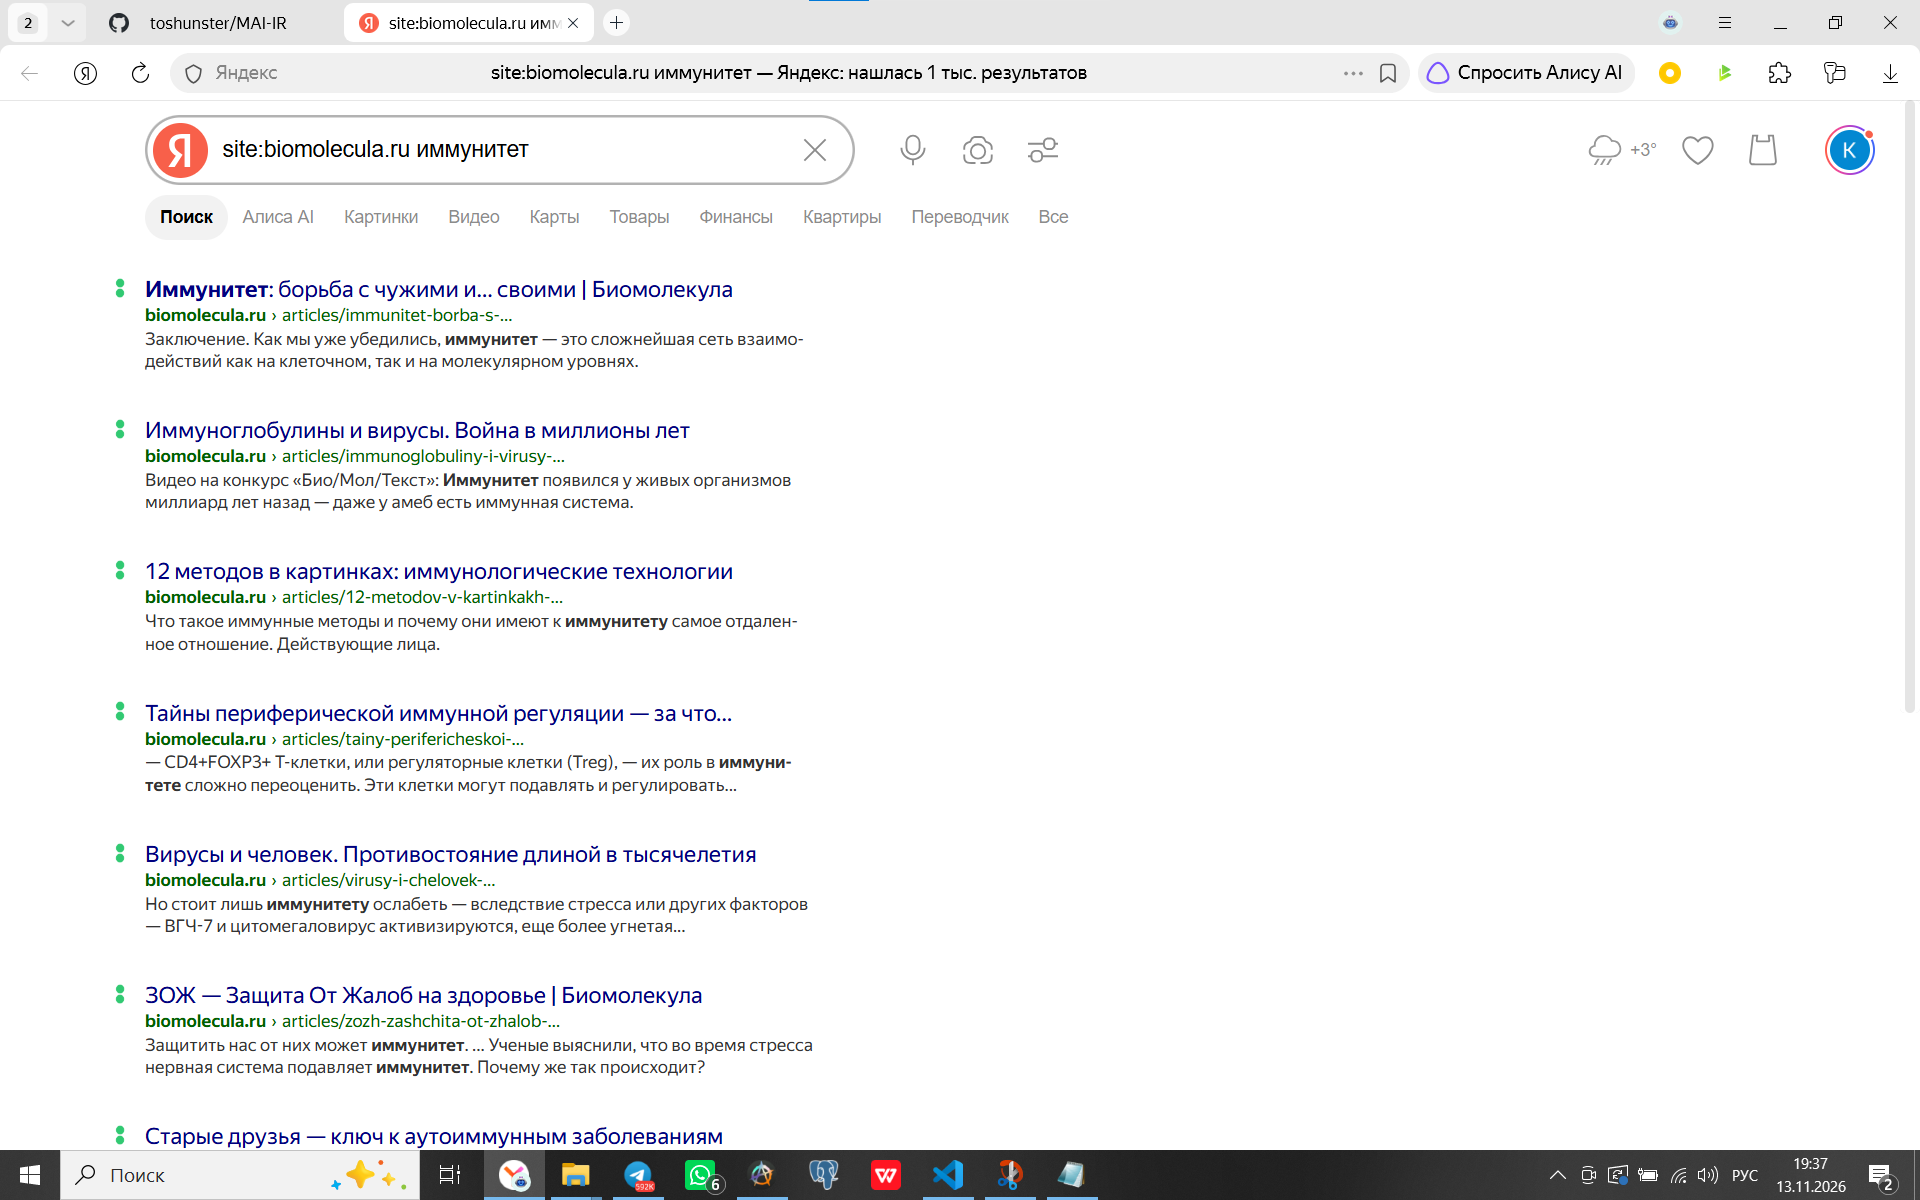
\includegraphics{images/screenshots/lab01_search_biomolecula.png}}
\setlength{\ScreenshotLeft}{0.05468750\wd\ScreenshotBox}
\setlength{\ScreenshotBottom}{0.32916667\ht\ScreenshotBox}
\setlength{\ScreenshotRight}{0.54166667\wd\ScreenshotBox}
\setlength{\ScreenshotTop}{0.09166667\ht\ScreenshotBox}
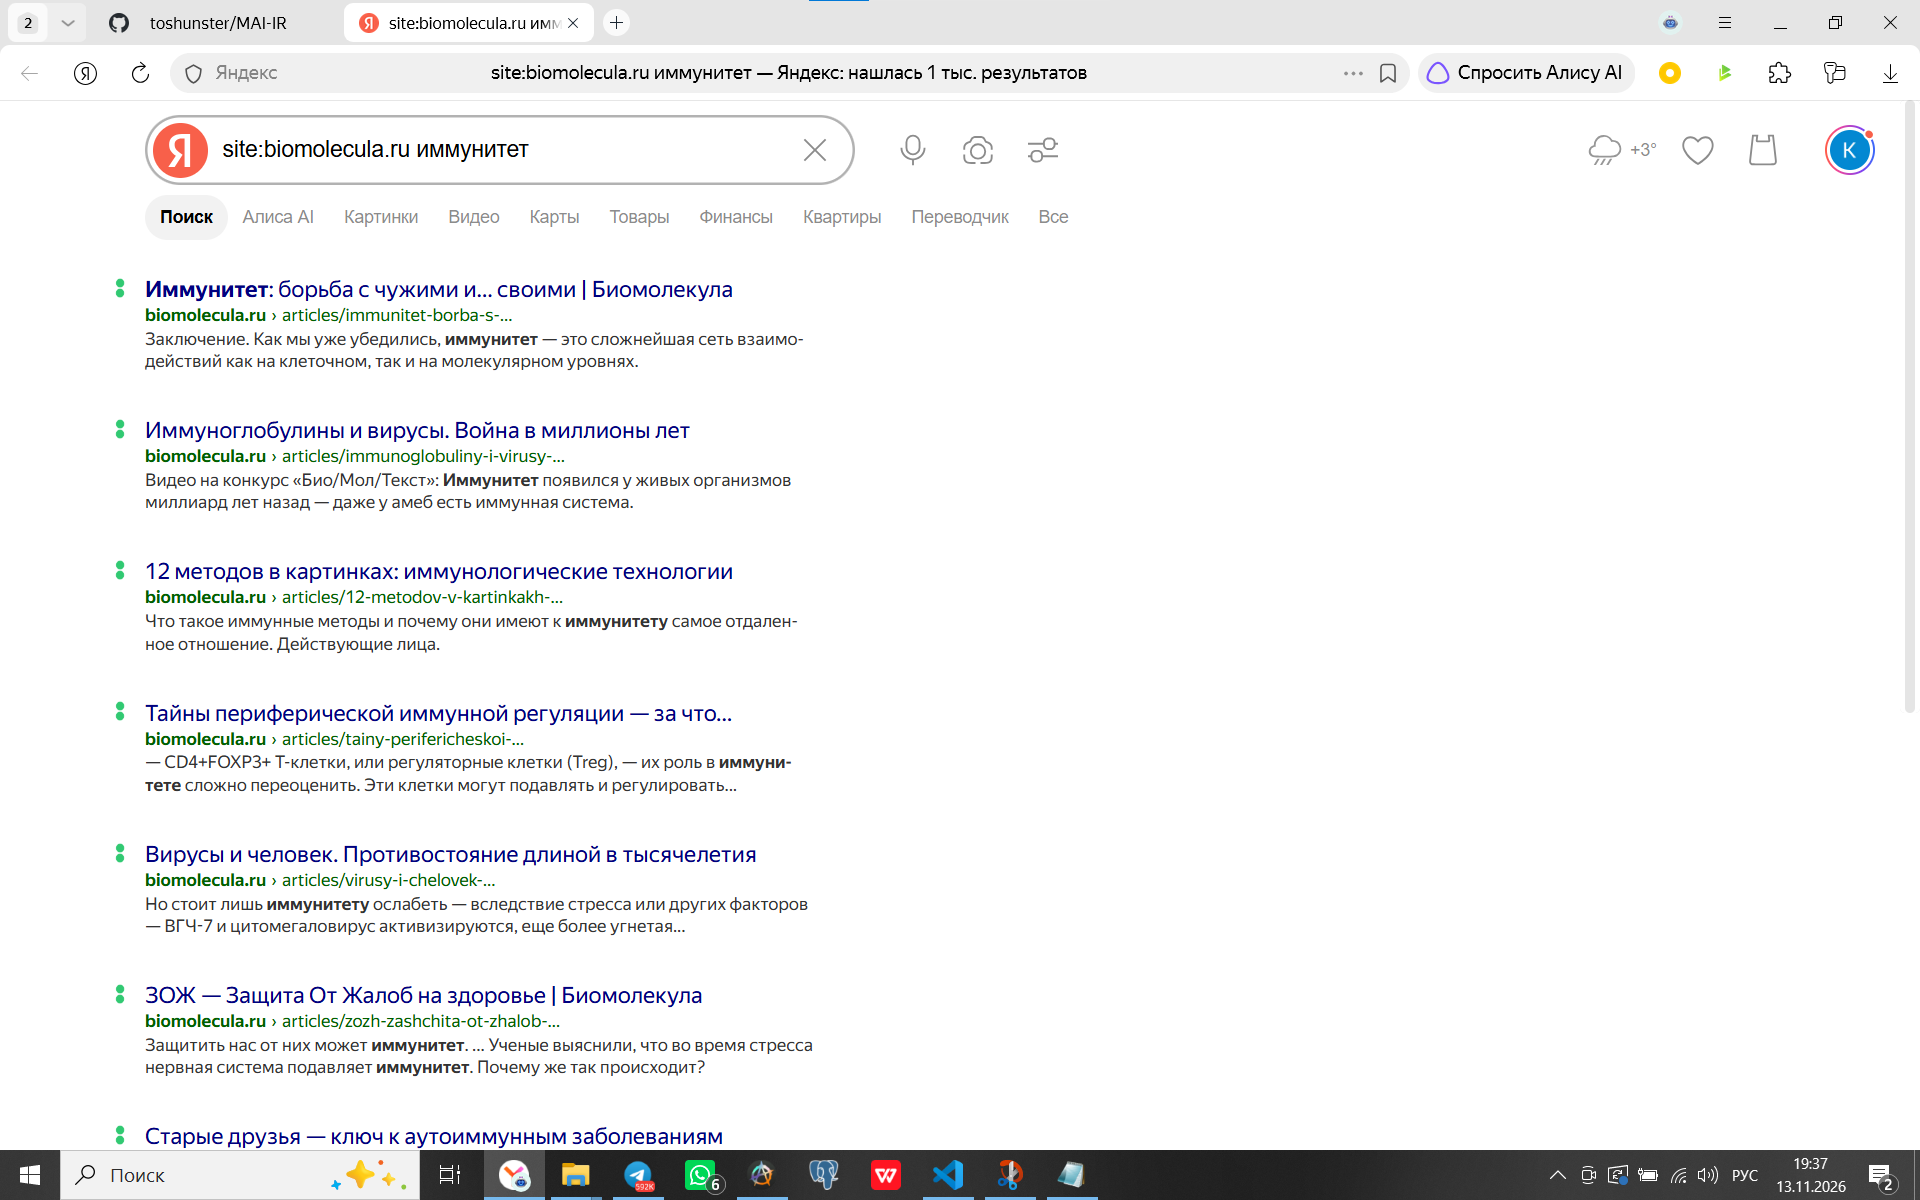
\includegraphics[trim={\ScreenshotLeft{} \ScreenshotBottom{} \ScreenshotRight{} \ScreenshotTop{}},clip,width=0.96\linewidth,height=0.70\textheight,keepaspectratio]{images/screenshots/lab01_search_biomolecula.png}
\endgroup\caption{Поиск по «Биомолекуле» в Яндексе}\end{figure}

\begin{figure}[H]\centering\begingroup
\sbox{\ScreenshotBox}{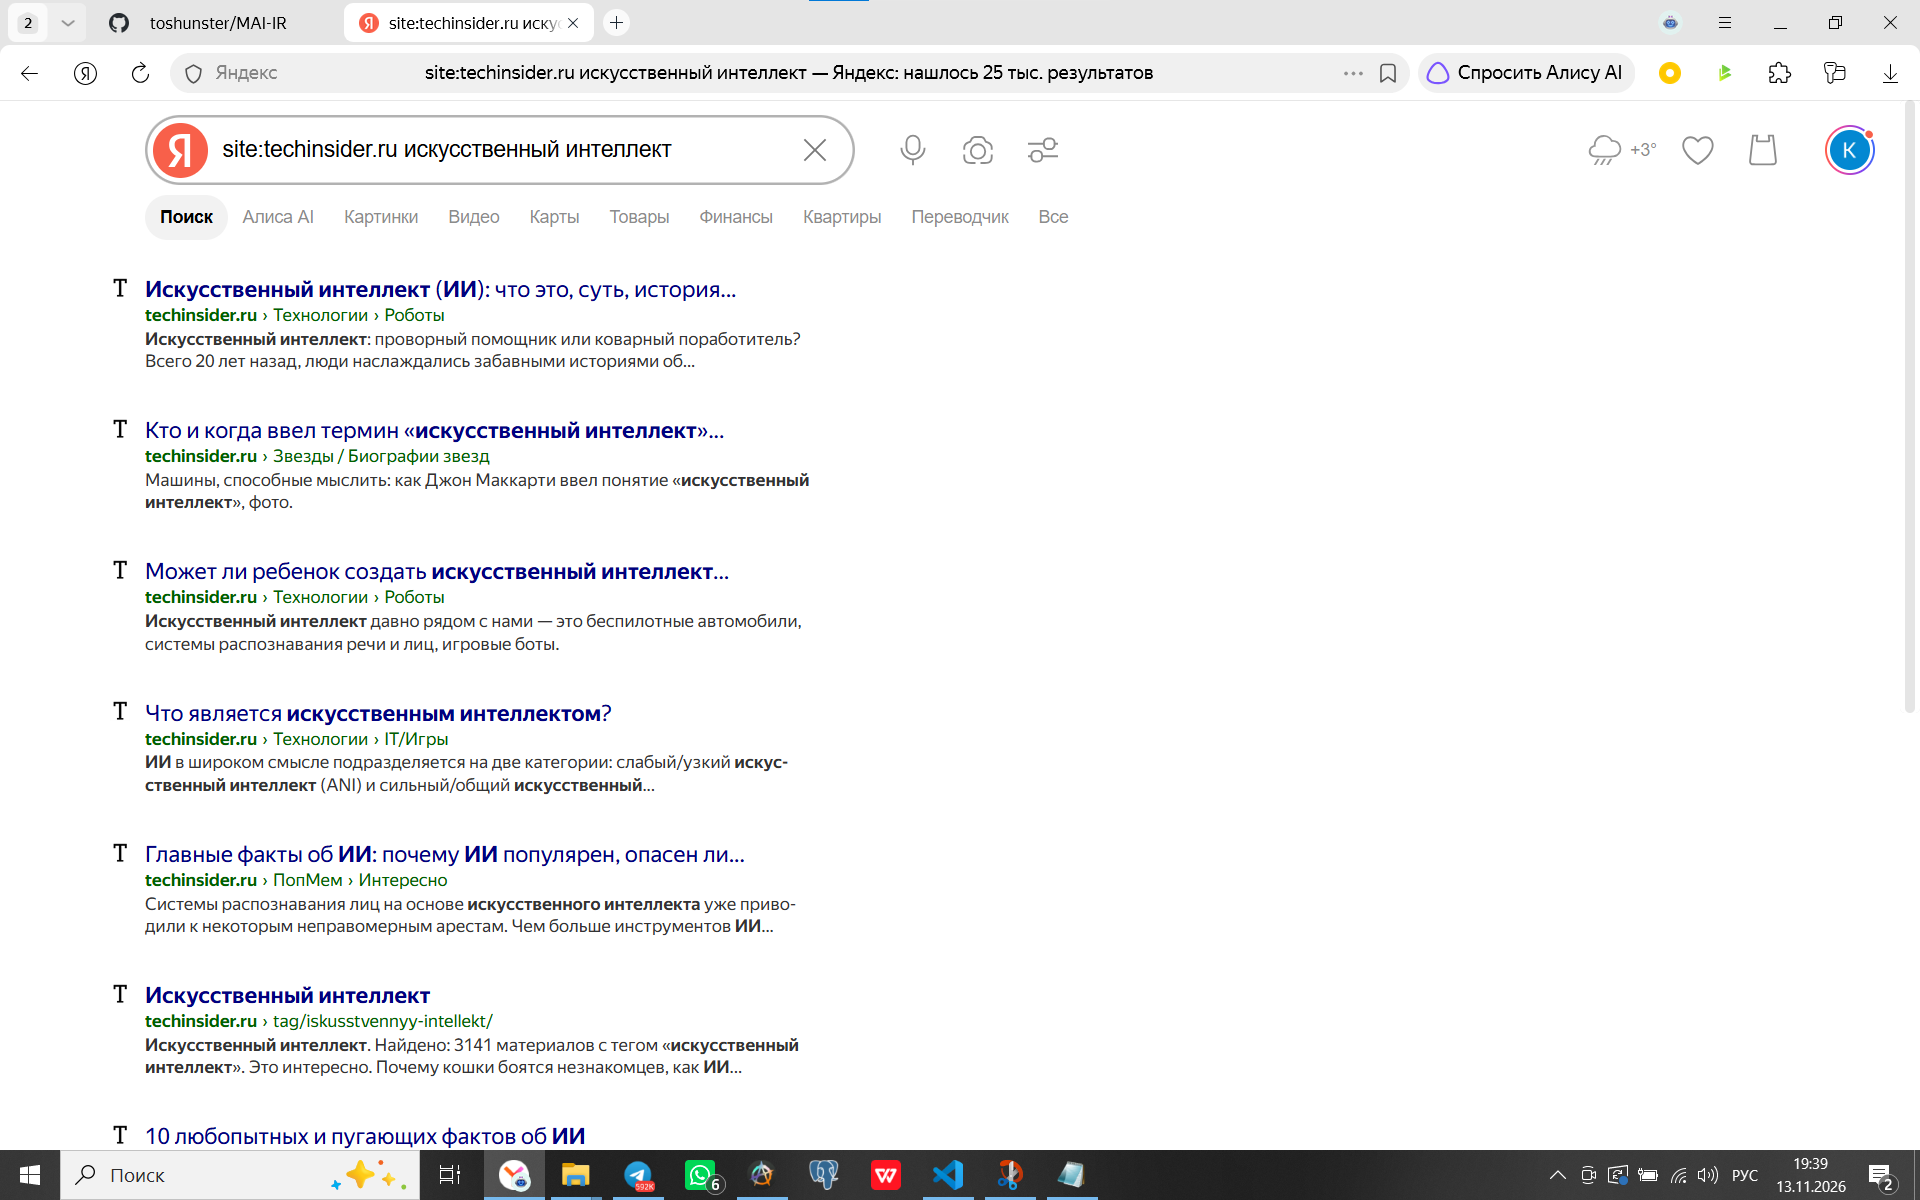
\includegraphics{images/screenshots/lab01_search_techinsider.png}}
\setlength{\ScreenshotLeft}{0.05468750\wd\ScreenshotBox}
\setlength{\ScreenshotBottom}{0.32916667\ht\ScreenshotBox}
\setlength{\ScreenshotRight}{0.54166667\wd\ScreenshotBox}
\setlength{\ScreenshotTop}{0.09166667\ht\ScreenshotBox}
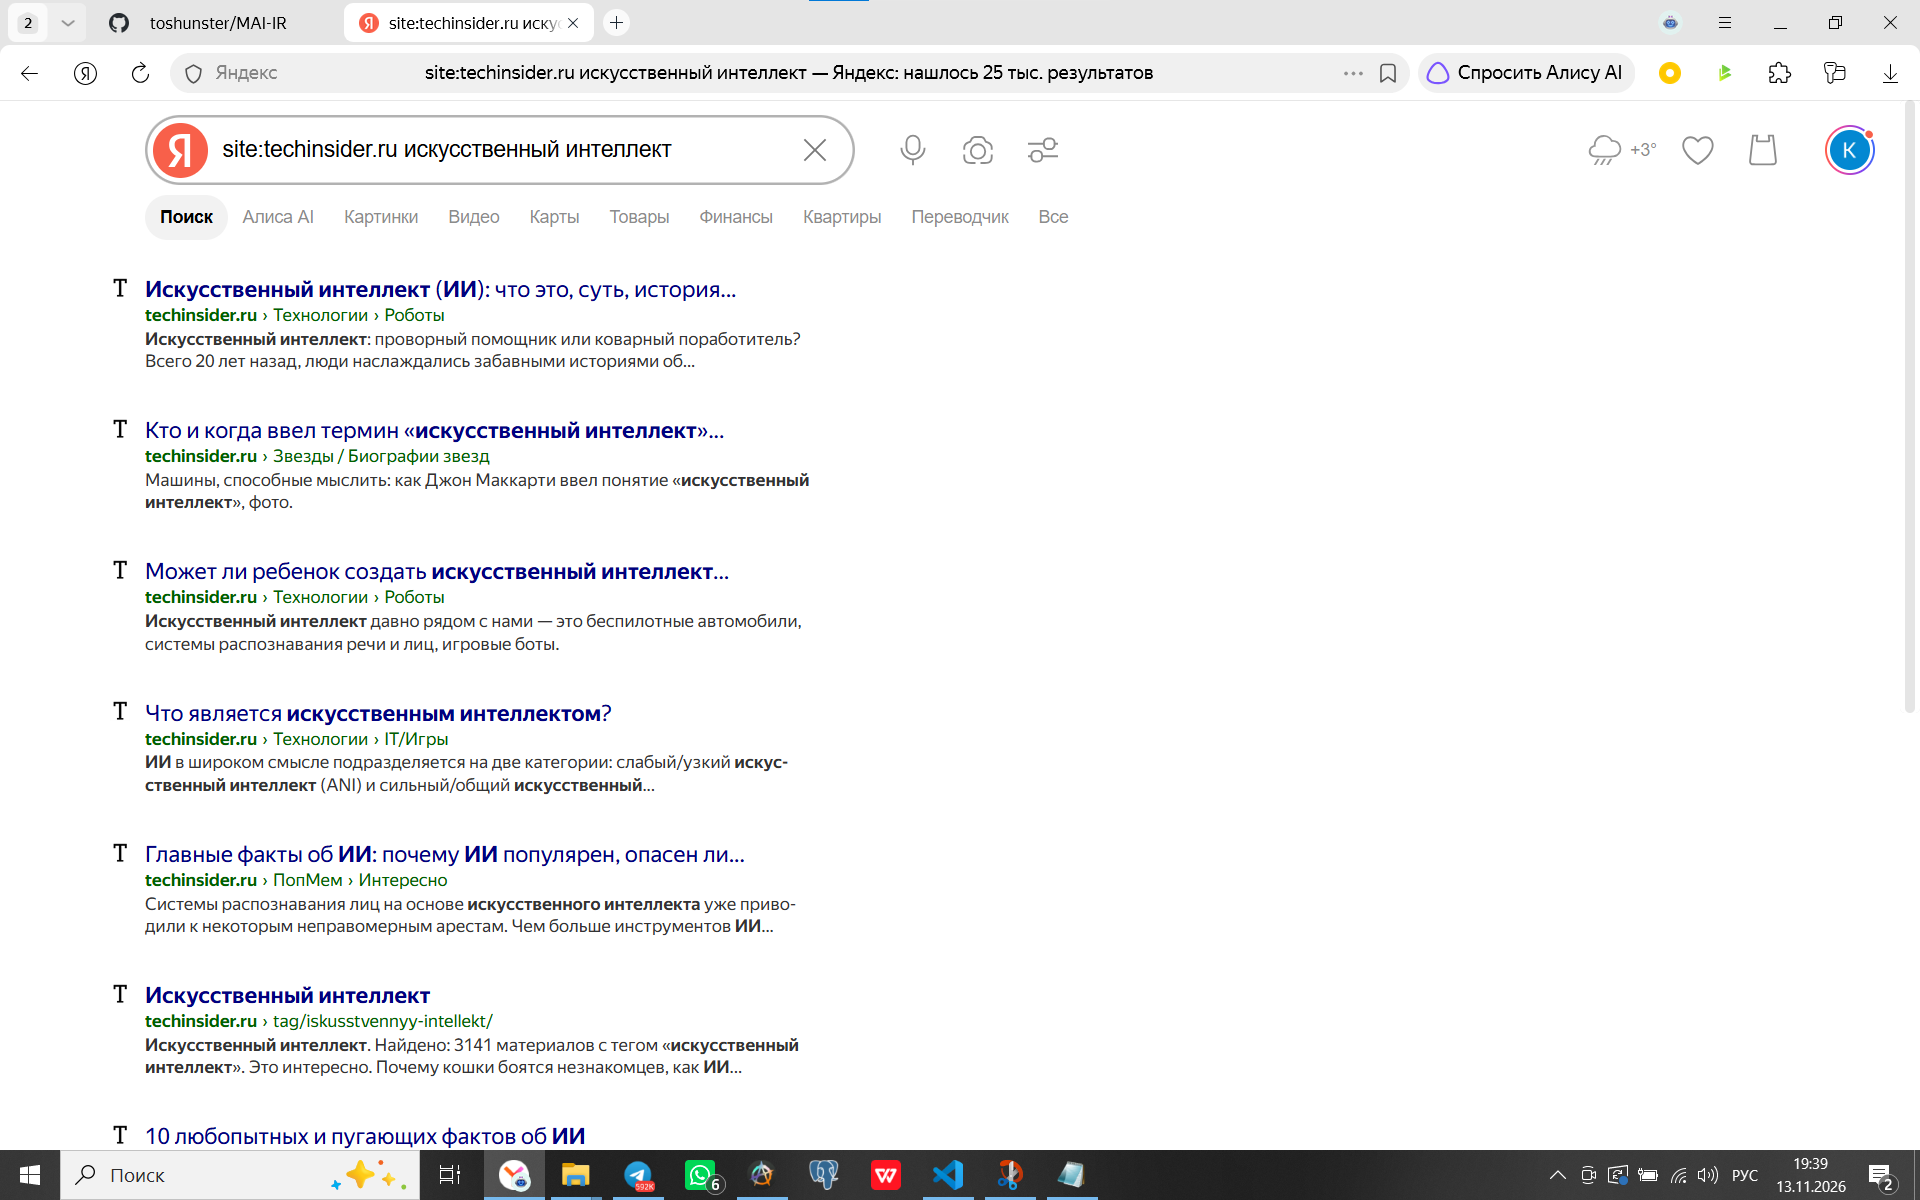
\includegraphics[trim={\ScreenshotLeft{} \ScreenshotBottom{} \ScreenshotRight{} \ScreenshotTop{}},clip,width=0.96\linewidth,height=0.70\textheight,keepaspectratio]{images/screenshots/lab01_search_techinsider.png}
\endgroup\caption{Поиск по TechInsider в Яндексе}\end{figure}

Внешний поиск может показывать служебные страницы и материалы со случайным упоминанием слов. Собственный поисковик позволяет управлять составом корпуса, булевыми условиями и точными цитатами. При этом качество собственной выдачи зависит от извлечения текста и выбранного ранжирования.
\sub{Объём корпуса}
\begin{table}[H]\centering\small
\caption{Характеристики корпуса документов}
\begin{tabularx}{\linewidth}{|X|r|}\hline
Показатель & Значение \\\hline
Количество документов & 992 743 \\\hline
Количество источников & 21 \\\hline
Объём выделенного UTF-8 текста, ГБ & 5,247 \\\hline
Средний объём текста документа, байт & 5 285 \\\hline
Среднее число токенов на документ & 402,5 \\\hline
Документы «Биомолекулы» & 3 580 \\\hline
Документы TechInsider & 116 443 \\\hline
Дата измерений & 2026-11-12 \\\hline
\end{tabularx}\end{table}
\begin{figure}[H]\centering\begingroup
\sbox{\ScreenshotBox}{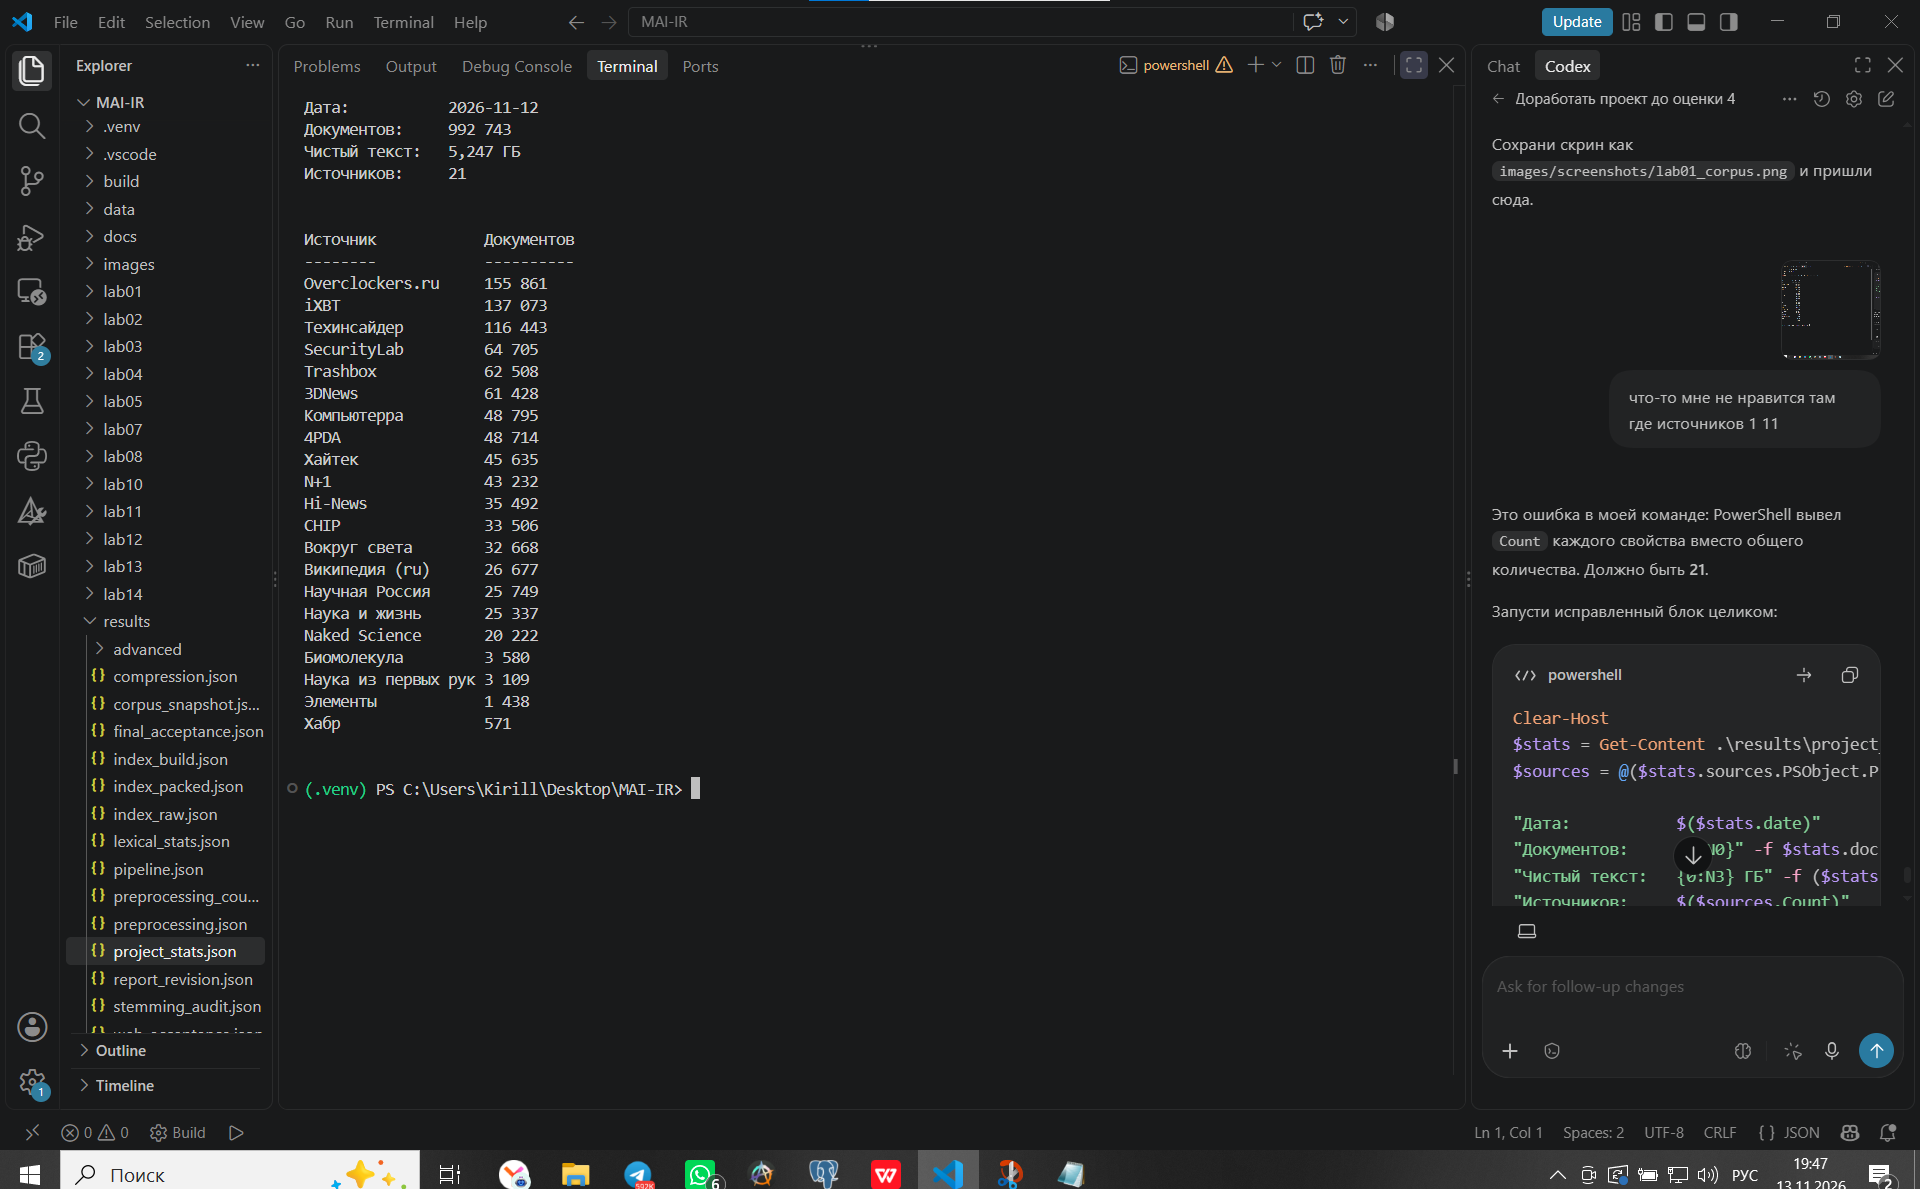
\includegraphics{images/screenshots/lab01_corpus.png}}
\setlength{\ScreenshotLeft}{0.15364583\wd\ScreenshotBox}
\setlength{\ScreenshotBottom}{0.37762826\ht\ScreenshotBox}
\setlength{\ScreenshotRight}{0.63020833\wd\ScreenshotBox}
\setlength{\ScreenshotTop}{0.07905803\ht\ScreenshotBox}
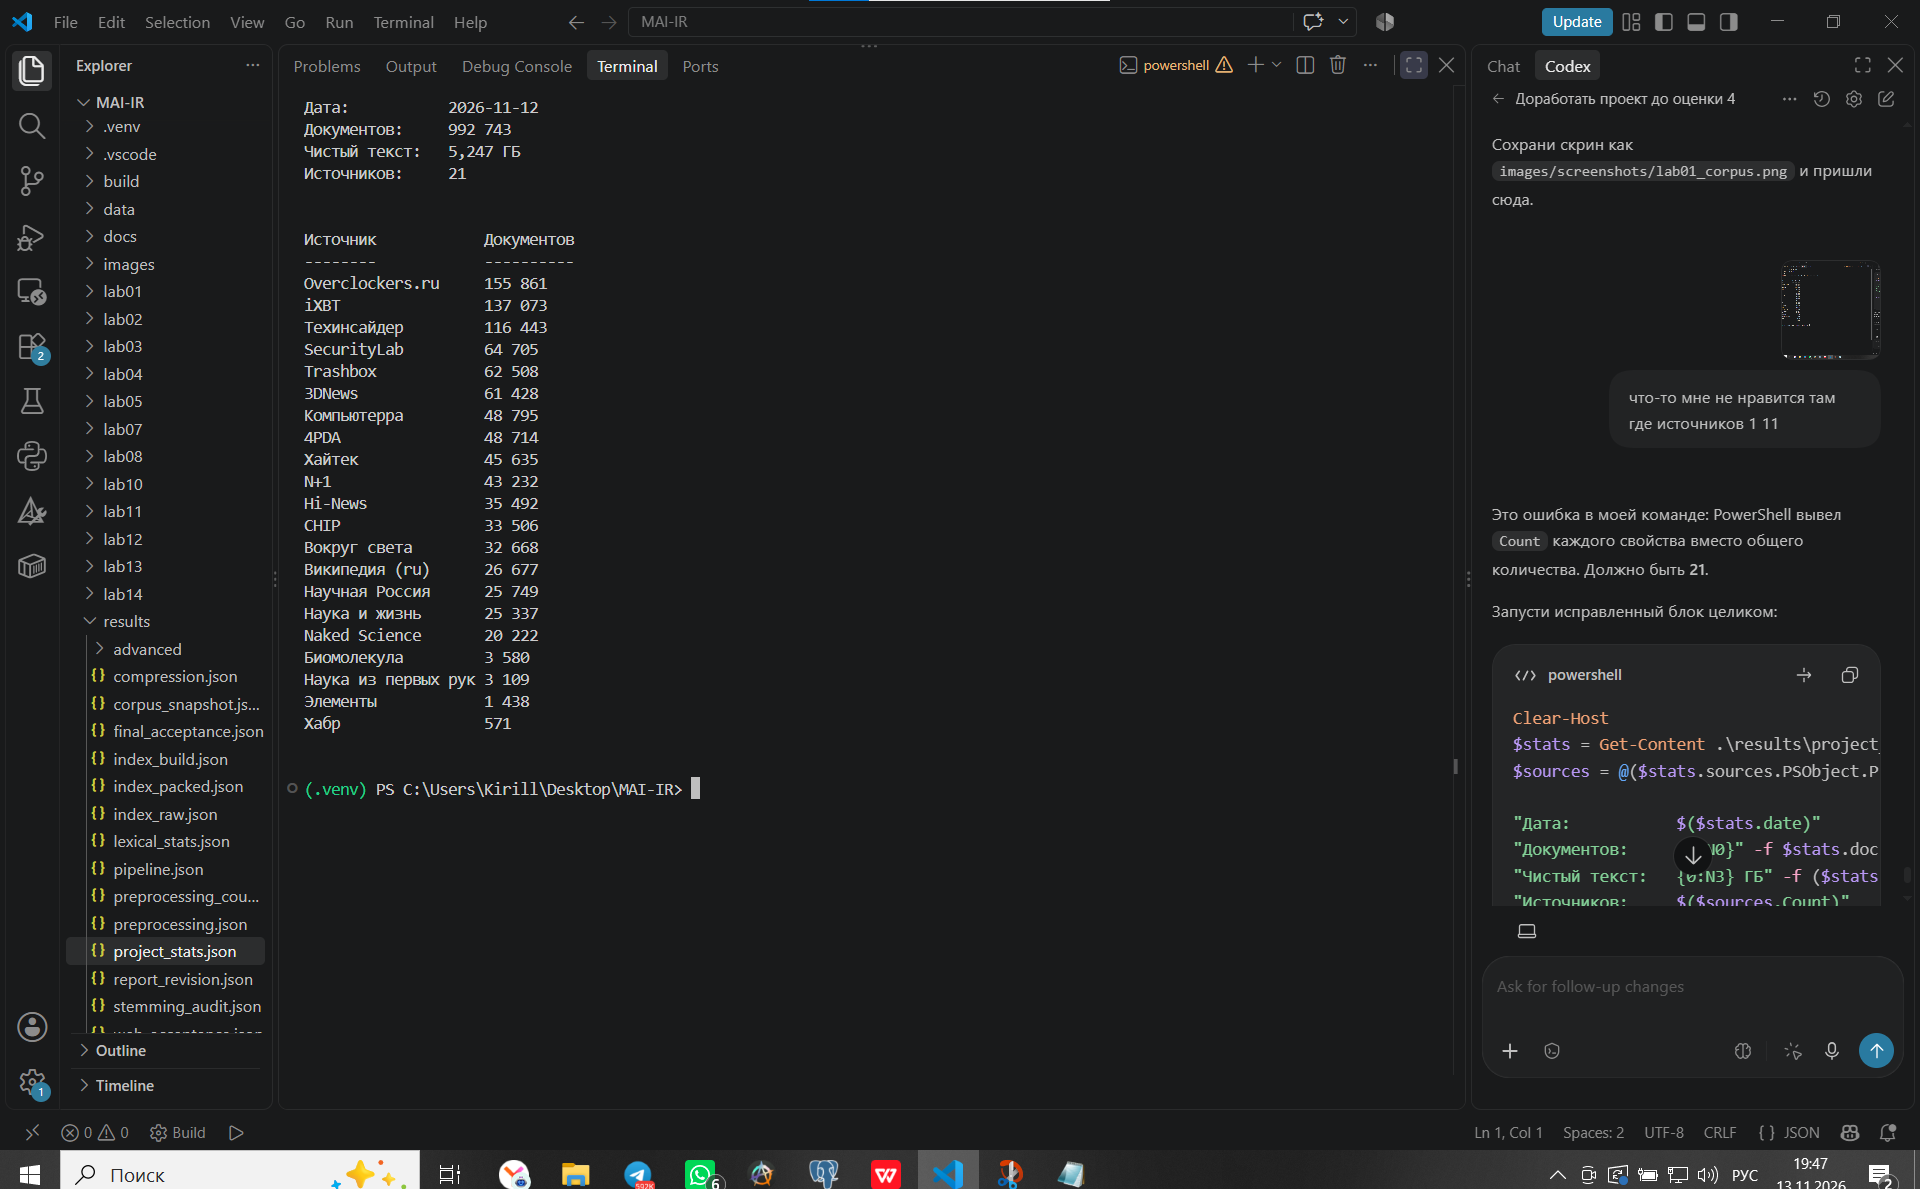
\includegraphics[trim={\ScreenshotLeft{} \ScreenshotBottom{} \ScreenshotRight{} \ScreenshotTop{}},clip,width=0.96\linewidth,height=0.70\textheight,keepaspectratio]{images/screenshots/lab01_corpus.png}
\endgroup\caption{Статистика корпуса документов}\end{figure}


\section{Лабораторная работа № 2\\«Поисковый робот»}
\sub{Настройки и запуск}
Робот загружает статьи и сохраняет их в PostgreSQL. Основная реализация: \code{lab02/crawler.py}. Для расширенного сбора по многим источникам используется \code{tools/collect_parallel.py}; источники и ограничения задаются в единственном \code{config.yaml}. Пароль БД хранится отдельно в локальном \code{.env}.

В конфигурации задаются соединение с БД, источники, число документов, задержки, ограничения и правила повторной проверки. У разных сайтов могут быть разные допустимые задержки. После установки зависимостей запуск выполняется из корня:
\begin{Verbatim}[fontsize=\small]
python lab02/crawler.py config.yaml
\end{Verbatim}
Расширенный сбор управляется командами \code{project.ps1 collect -Background}, \code{collect -Summary} и \code{collect -Stop}. Для демонстрации уже собранного корпуса повторный сетевой обход не требуется.
\sub{Загрузка и хранение}
Очередь содержит нормализованные URL. Робот пропускает известные адреса, проверяет пригодность страницы, получает HTML и извлекает статью. Сетевые ошибки и неподходящие страницы учитываются без остановки всего сбора. Основные поля таблицы \code{documents}:
\begin{longtable}{|p{58mm}|p{91mm}|}
\caption{Хранимые данные документа}\\\hline
Поле & Назначение \\\hline\endfirsthead
\hline Поле & Назначение \\\hline\endhead
\code{id} & Идентификатор записи \\\hline
\code{url}, \code{normalized_url} & Исходный и нормализованный адреса; нормализованный URL уникален \\\hline
\code{html}, \code{clean_text} & HTML и выделенный основной текст \\\hline
\code{title}, \code{author}, \code{publish_date} & Заголовок, авторы и дата публикации \\\hline
\code{source} & Источник статьи \\\hline
\code{fetch_timestamp}, \code{last_fetch_attempt} & Время сохранения и последней проверки \\\hline
\code{last_modified_header}, \code{etag_header} & Заголовки для условного HTTP-запроса \\\hline
\end{longtable}
\sub{Остановка и продолжение}
Очередь и счётчик сохранённых документов записываются в файл состояния. При Ctrl+C робот завершает текущую операцию и сохраняет состояние; следующий запуск продолжает обработку. Уже имеющиеся в БД адреса пропускаются. Базовый робот использует \code{crawler_state.pkl}, расширенный сборщик --- своё состояние очереди. Это разные режимы запуска одной задачи сбора.
\sub{Обновление документов}
Период повторной проверки задаётся параметром \code{update_interval_seconds}. При наличии ETag и Last-Modified выполняется условный запрос. Ответ 304 обновляет время проверки. При ответе 200 сравнивается MD5 от заголовка, авторов, даты и текста: если содержание изменилось, запись обновляется. Изменение одной HTML-разметки при прежнем тексте не требует перезаписи статьи.

Для отдельной проверки сохранённых статей предусмотрен режим \code{--update-only}. Параметр \code{--limit 3} ограничивает выборку тремя статьями, \code{--update-interval 0} отменяет ожидание только на этот запуск. Конфигурационный файл при этом не изменяется. В приведённом запуске серверы вернули HTTP 200: одна запись обновлена, у двух содержимое совпало.
\sub{Проверки и результаты}
Проверки охватывают нормализацию URL, извлечение текста и метаданных, сохранение очереди, продолжение обработки, сетевые отказы и ограничения источников. Изолированные автотесты сборщика включены в общий запуск; результаты сохранены в \code{tests/results/collection.txt}. Состояние документов и очереди можно проверить отдельно от сетевой загрузки.
\begin{figure}[H]\centering\begingroup
\sbox{\ScreenshotBox}{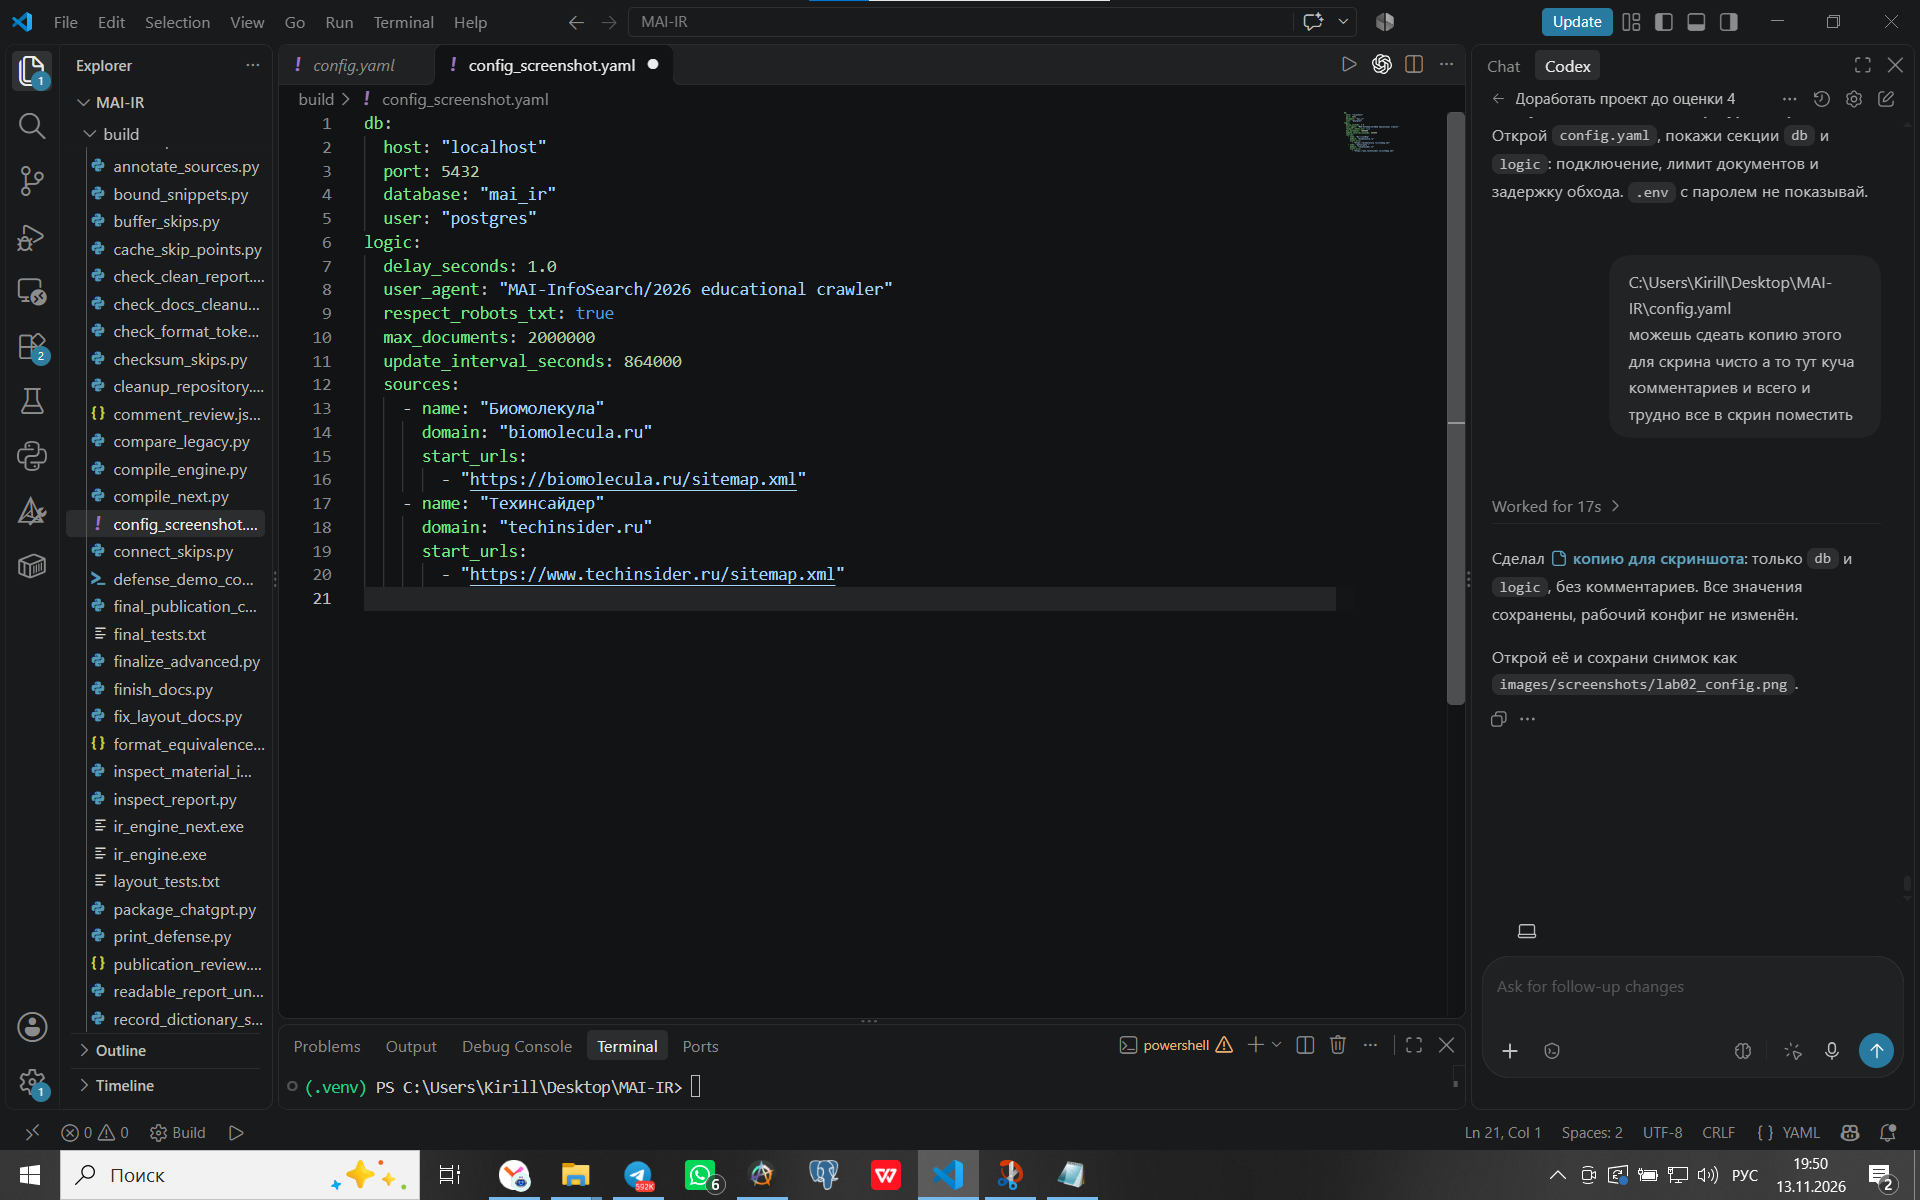
\includegraphics{images/screenshots/lab02_config.png}}
\setlength{\ScreenshotLeft}{0.18750000\wd\ScreenshotBox}
\setlength{\ScreenshotBottom}{0.51333333\ht\ScreenshotBox}
\setlength{\ScreenshotRight}{0.47916667\wd\ScreenshotBox}
\setlength{\ScreenshotTop}{0.09166667\ht\ScreenshotBox}
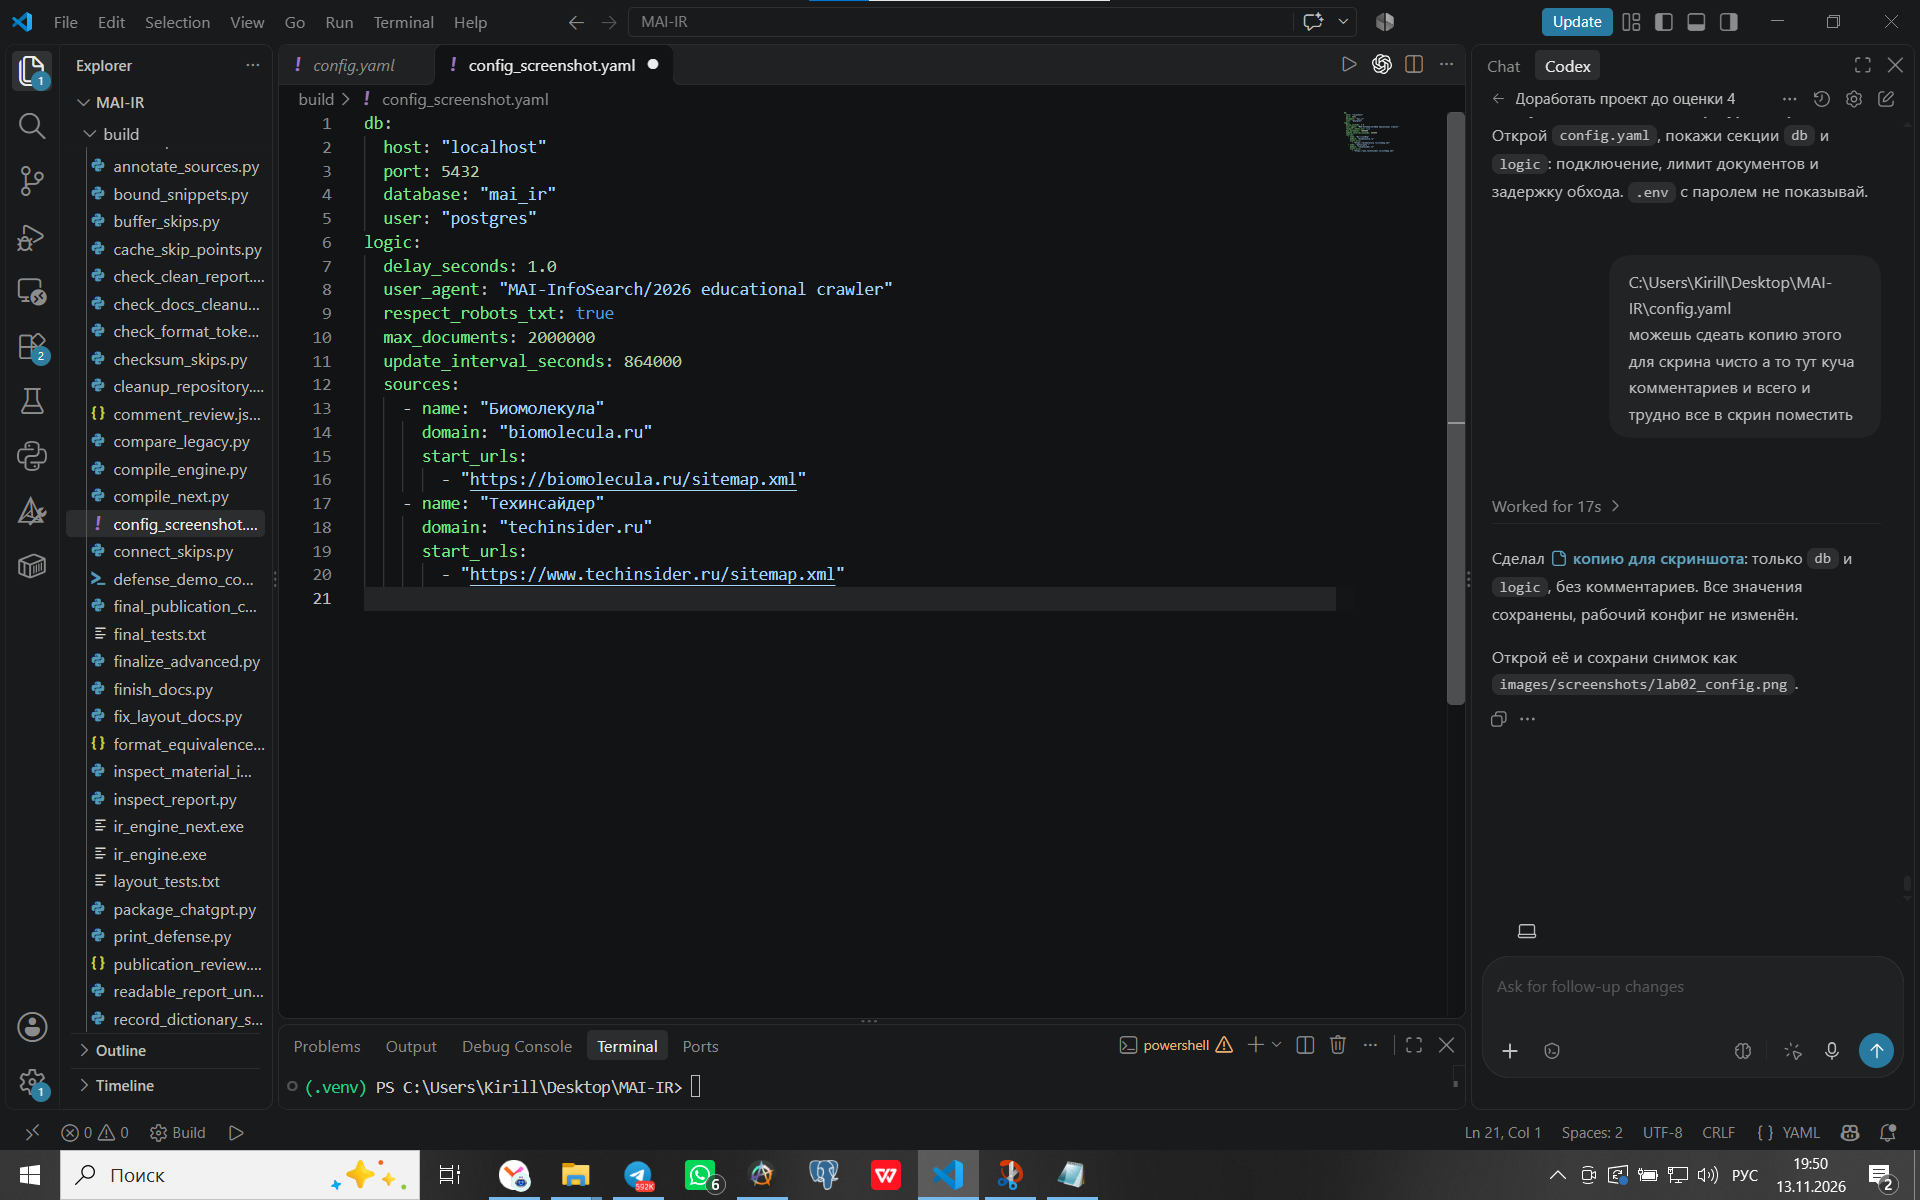
\includegraphics[trim={\ScreenshotLeft{} \ScreenshotBottom{} \ScreenshotRight{} \ScreenshotTop{}},clip,width=0.96\linewidth,height=0.70\textheight,keepaspectratio]{images/screenshots/lab02_config.png}
\endgroup\caption{Пример параметров базового робота: подключение и обход двух источников}\end{figure}
\begin{figure}[H]\centering\begingroup
\sbox{\ScreenshotBox}{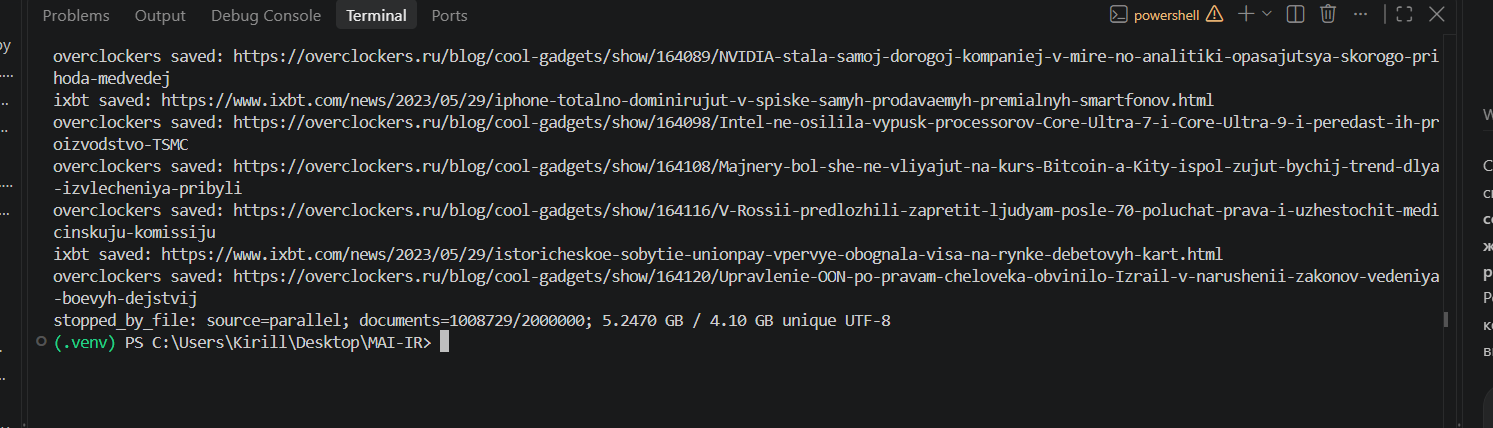
\includegraphics{images/screenshots/lab02_run.png}}
\setlength{\ScreenshotLeft}{0.03081045\wd\ScreenshotBox}
\setlength{\ScreenshotBottom}{0.22429907\ht\ScreenshotBox}
\setlength{\ScreenshotRight}{0.21634293\wd\ScreenshotBox}
\setlength{\ScreenshotTop}{0.09345794\ht\ScreenshotBox}
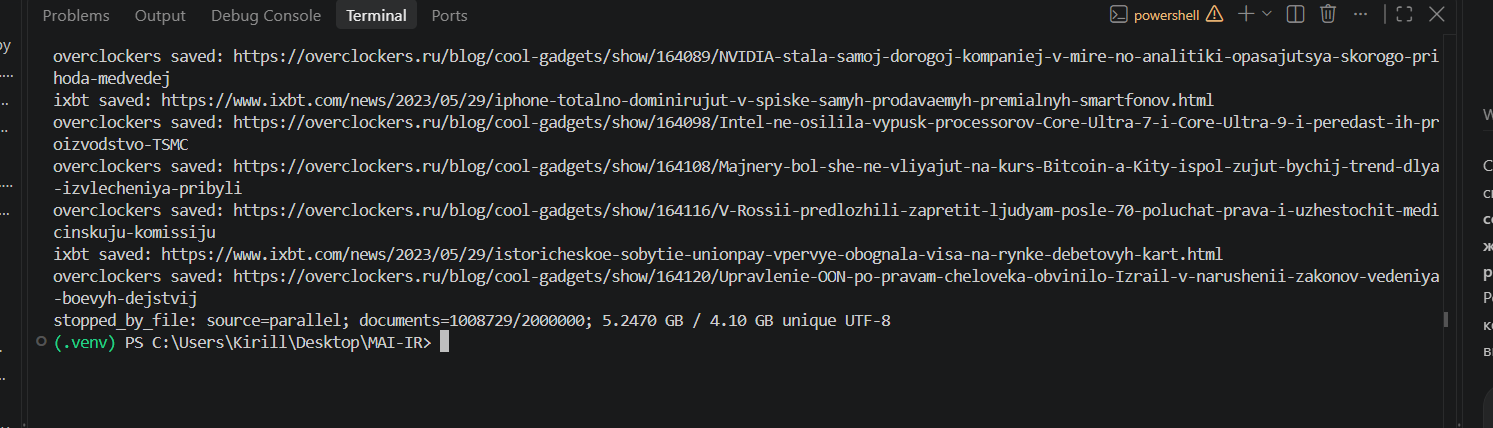
\includegraphics[trim={\ScreenshotLeft{} \ScreenshotBottom{} \ScreenshotRight{} \ScreenshotTop{}},clip,width=0.96\linewidth,height=0.70\textheight,keepaspectratio]{images/screenshots/lab02_run.png}
\endgroup\caption{Фрагмент сохранённого журнала сбора документов}\end{figure}
\begin{figure}[H]\centering\begingroup
\sbox{\ScreenshotBox}{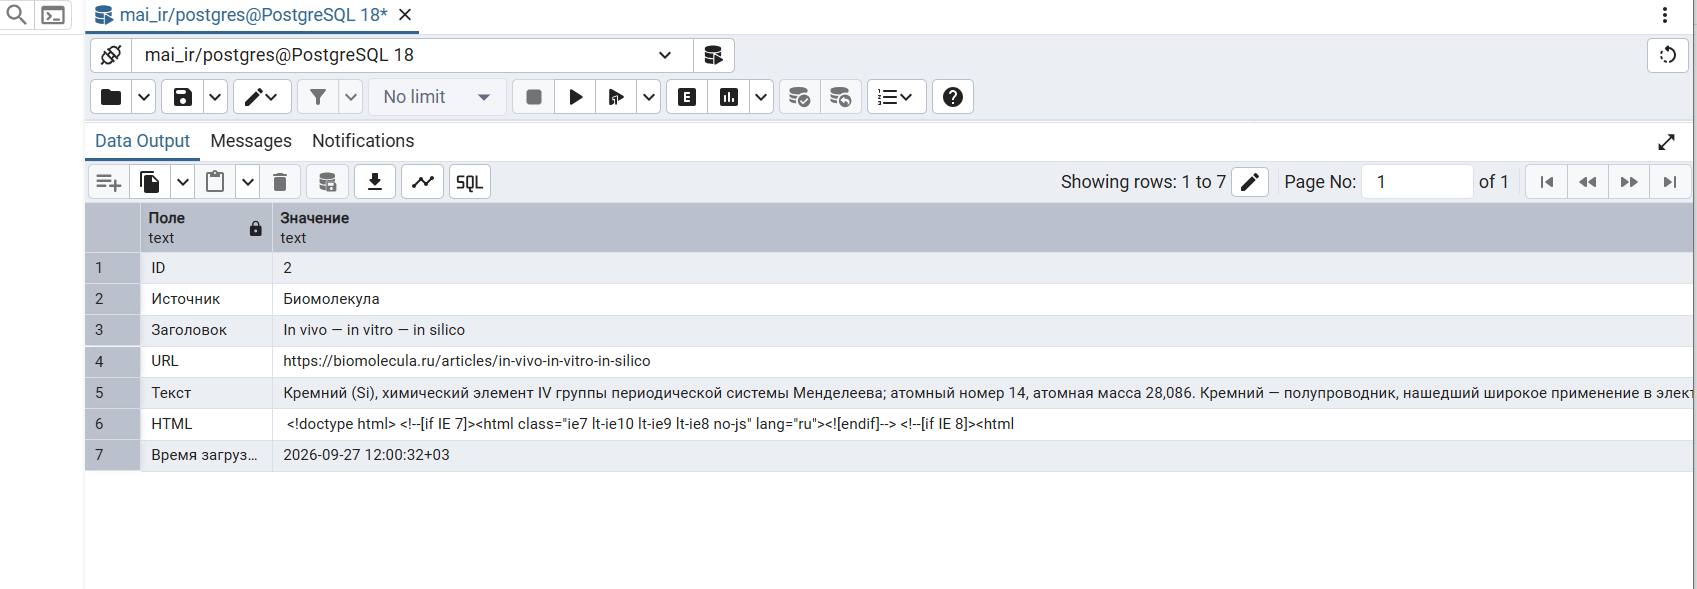
\includegraphics{images/screenshots/lab02_database.png}}
\setlength{\ScreenshotLeft}{0.08249853\wd\ScreenshotBox}
\setlength{\ScreenshotBottom}{0.19694397\ht\ScreenshotBox}
\setlength{\ScreenshotRight}{0.38126105\wd\ScreenshotBox}
\setlength{\ScreenshotTop}{0.34295416\ht\ScreenshotBox}
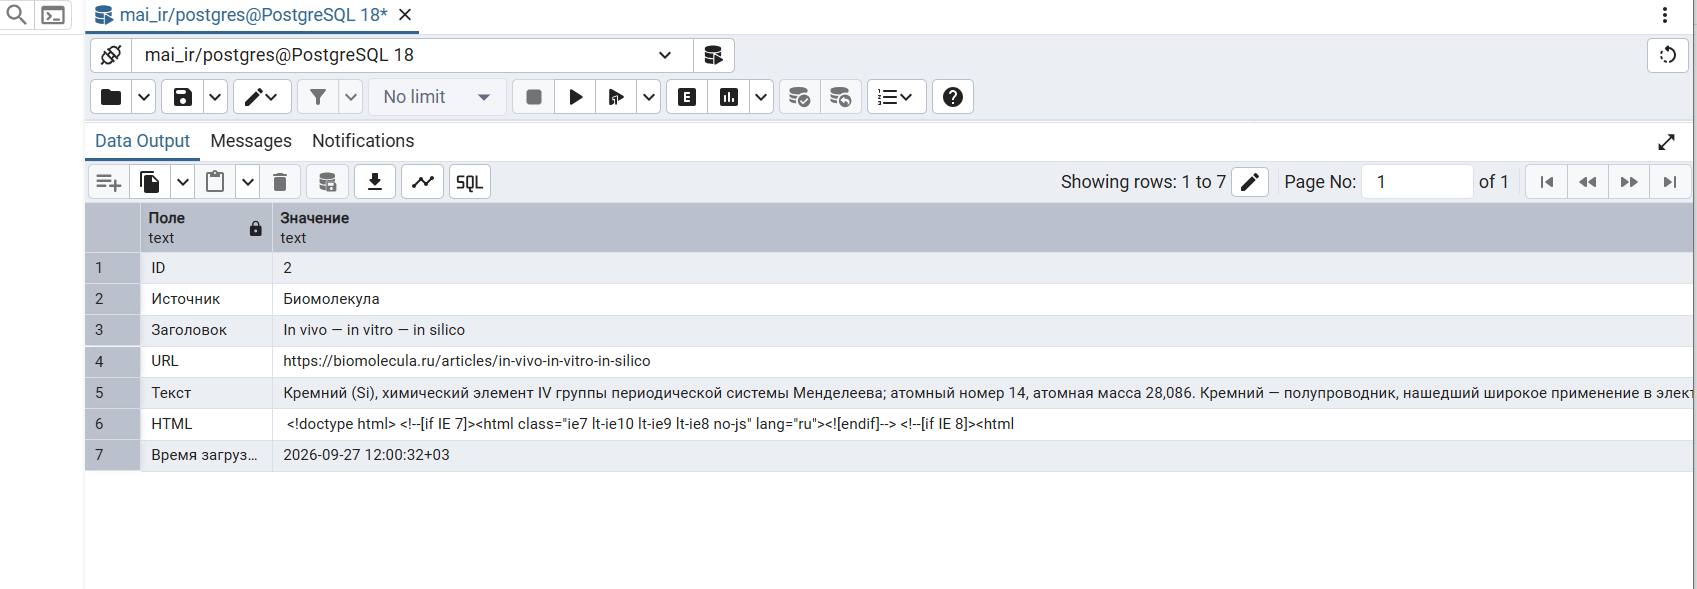
\includegraphics[trim={\ScreenshotLeft{} \ScreenshotBottom{} \ScreenshotRight{} \ScreenshotTop{}},clip,width=0.96\linewidth,height=0.70\textheight,keepaspectratio]{images/screenshots/lab02_database.png}
\endgroup\caption{Документ и его метаданные в PostgreSQL}\end{figure}
\begin{figure}[H]\centering\begingroup
\sbox{\ScreenshotBox}{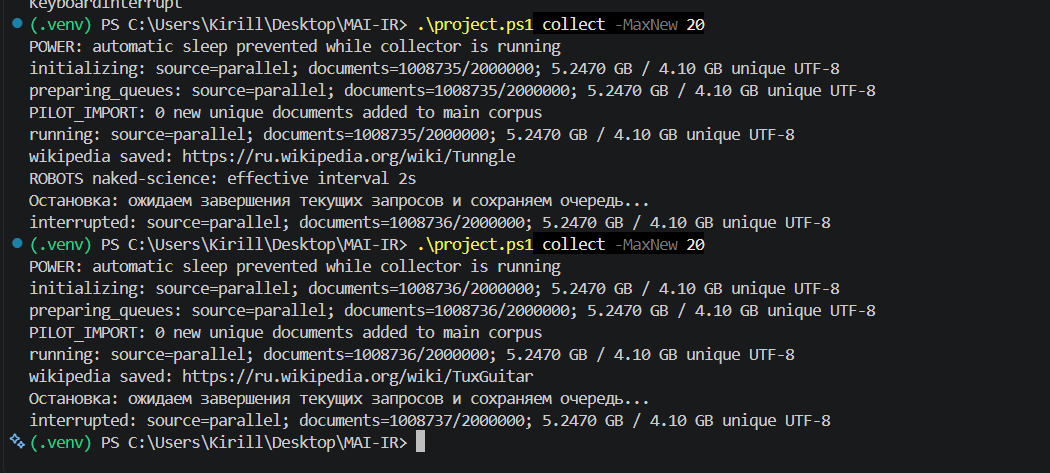
\includegraphics{images/screenshots/lab02_resume.png}}
\setlength{\ScreenshotLeft}{0.02380952\wd\ScreenshotBox}
\setlength{\ScreenshotBottom}{0.09090909\ht\ScreenshotBox}
\setlength{\ScreenshotRight}{0.00952381\wd\ScreenshotBox}
\setlength{\ScreenshotTop}{0.03805497\ht\ScreenshotBox}
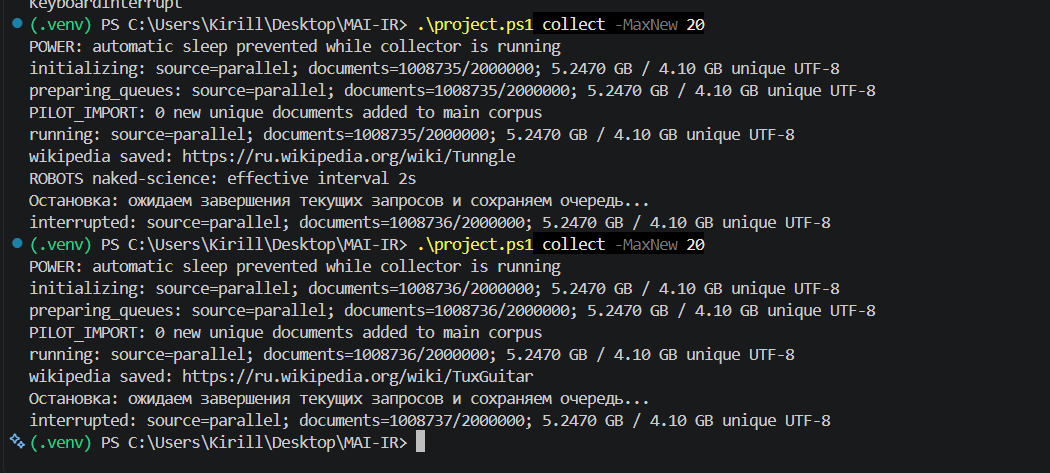
\includegraphics[trim={\ScreenshotLeft{} \ScreenshotBottom{} \ScreenshotRight{} \ScreenshotTop{}},clip,width=0.96\linewidth,height=0.70\textheight,keepaspectratio]{images/screenshots/lab02_resume.png}
\endgroup\caption{Остановка и продолжение работы с сохранённой очередью}\end{figure}
\begin{figure}[H]\centering\begingroup
\sbox{\ScreenshotBox}{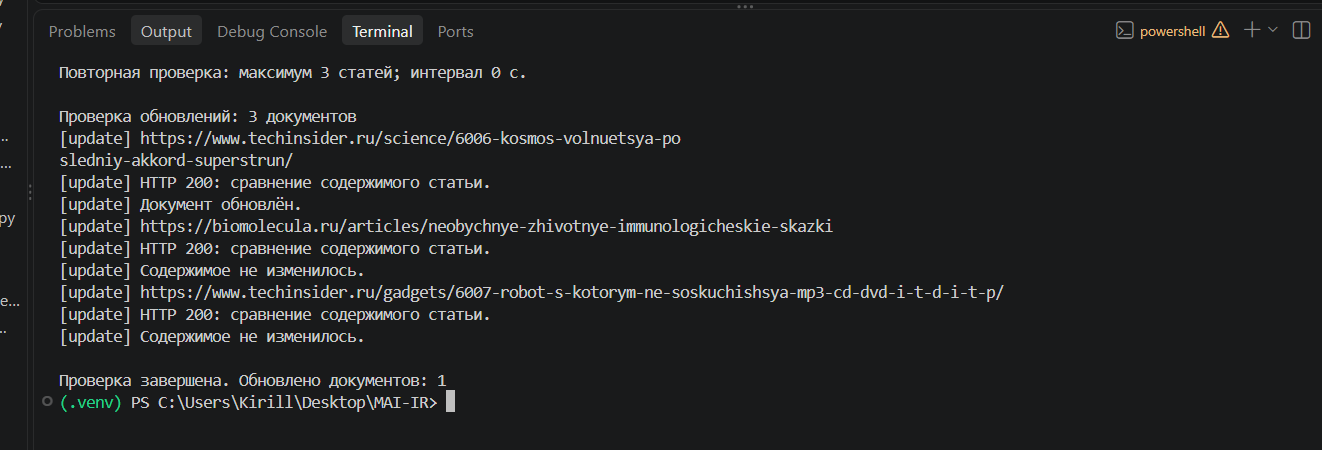
\includegraphics{images/screenshots/lab02_update.png}}
\setlength{\ScreenshotLeft}{0.03933434\wd\ScreenshotBox}
\setlength{\ScreenshotBottom}{0.12888889\ht\ScreenshotBox}
\setlength{\ScreenshotRight}{0.21331316\wd\ScreenshotBox}
\setlength{\ScreenshotTop}{0.13333333\ht\ScreenshotBox}
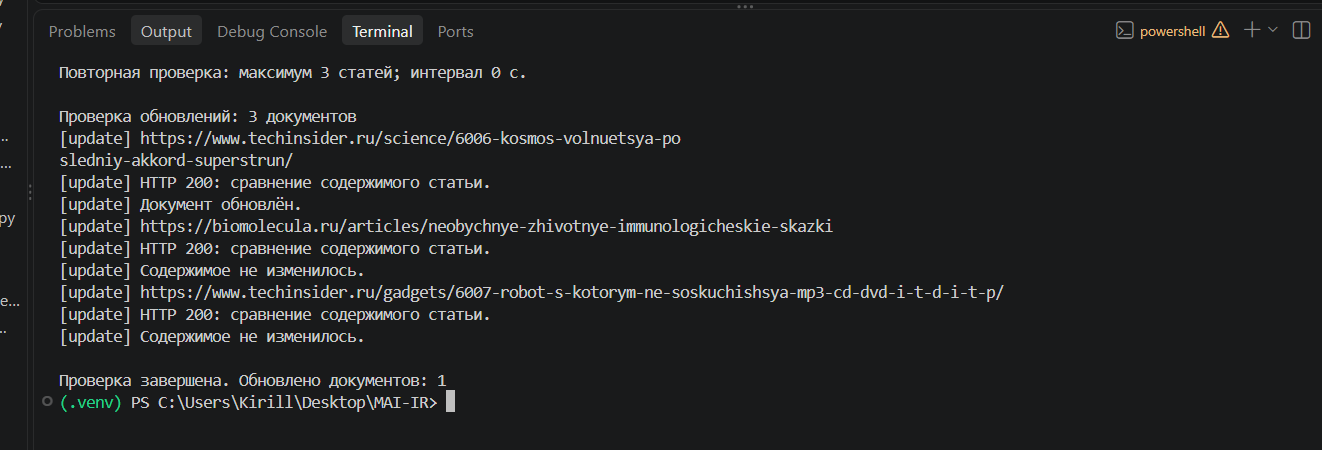
\includegraphics[trim={\ScreenshotLeft{} \ScreenshotBottom{} \ScreenshotRight{} \ScreenshotTop{}},clip,width=0.96\linewidth,height=0.70\textheight,keepaspectratio]{images/screenshots/lab02_update.png}
\endgroup\caption{Повторная проверка трёх статей: одна запись обновлена}\end{figure}
Счётчики в журналах отражают состояние сбора в PostgreSQL. Поисковый индекс построен по отдельному согласованному снимку из 992 743 документов; продолжение сбора не изменяет готовый индекс автоматически.

\sub{Экспорт для поиска}
Экспорт \code{lab03/export_texts.py --stream} читает БД серверным курсором и создаёт \code{data/corpus/texts.tsv}. Строка содержит ID, текст, заголовок и URL; внутренние переводы строк и TAB заменяются пробелами. База используется для сбора, поиск выполняется по собственному бинарному индексу. Базовый пересчёт запускается командой \code{project.ps1 rebuild}, подготовка лемм, координат, прыжков и данных сниппетов --- \code{project.ps1 upgrade}.


\section{Лабораторная работа № 3\\«Токенизация»}
\sub{Задание и метод}
Токенизатор делит UTF-8 текст на слова и обозначения, приводит регистр и сохраняет порядок и повторы. Основной код: \code{lab03/funcs/tokenizer.cpp}. Один документ обрабатывается за раз.

Сохраняются русские и латинские слова, числа и буквенно-цифровые обозначения. Ведущие нули значимы: \code{007} и \code{7} --- разные токены. Дефис внутри обозначения сохраняется, например \code{COVID-19}; тире, пунктуация и эмодзи разделяют токены. Аббревиатуры приводятся к записи из списка. Стоп-слова в основном конвейере не удаляются: они нужны в том числе для точных цитат. Например, «Компьютеры, 007 и COVID-19!» превращается в последовательность «компьютеры 007 и covid-19» с учётом настроенного списка аббревиатур.
\sub{Проверки}
Тесты покрывают пустой ввод, оба алфавита, регистр, числа, ведущие нули, дефисы, длинные слова, повторы, конец файла и неверный UTF-8. Проверяются функции C++ и консольная программа. Ожидания и граничные случаи описаны в \code{tests_lr3_4/TEST_PLAN.md}.
\sub{Измерения}

\begin{table}[H]\centering\small
\caption{Статистика токенизации и стемминга}
\begin{tabularx}{\linewidth}{|X|r|}\hline
Показатель & Значение \\\hline
Документов & 992 743 \\\hline
Объём текстов, МБ & 5 247,09 \\\hline
Вхождений токенов & 399 609 278 \\\hline
Уникальных токенов & 3 028 209 \\\hline
Средняя длина токена, символов (с повторами) & 6,132 \\\hline
Средняя длина уникального токена, символов & 11,474 \\\hline
Вхождений основ & 399 609 278 \\\hline
Уникальных основ & 1 963 565 \\\hline
Средняя длина уникальной основы, символов & 11,725 \\\hline
Сокращение словаря после стемминга, \% & 35,16 \\\hline
Число объединённых элементов словаря (V − S) & 1 064 644 \\\hline
Отношение размеров словарей V/S & 1,542 \\\hline
Изменённых вхождений после стемминга, \% & 62,53 \\\hline
Реализаций стеммера & 1 (русский Snowball / Porter) \\\hline
\end{tabularx}\end{table}

\begin{table}[H]\centering\small
\caption{Токенизация: медиана пяти повторов без файлового ввода-вывода}
\begin{tabularx}{\linewidth}{|X|r|r|}\hline
Текст, МБ & Секунды & МБ/с \\\hline
2,10 & 0,0291 & 72,14 \\\hline
5,25 & 0,0710 & 73,93 \\\hline
10,50 & 0,1461 & 71,88 \\\hline
15,75 & 0,2300 & 68,48 \\\hline
21,00 & 0,2921 & 71,88 \\\hline
\end{tabularx}\end{table}

\begin{figure}[H]\centering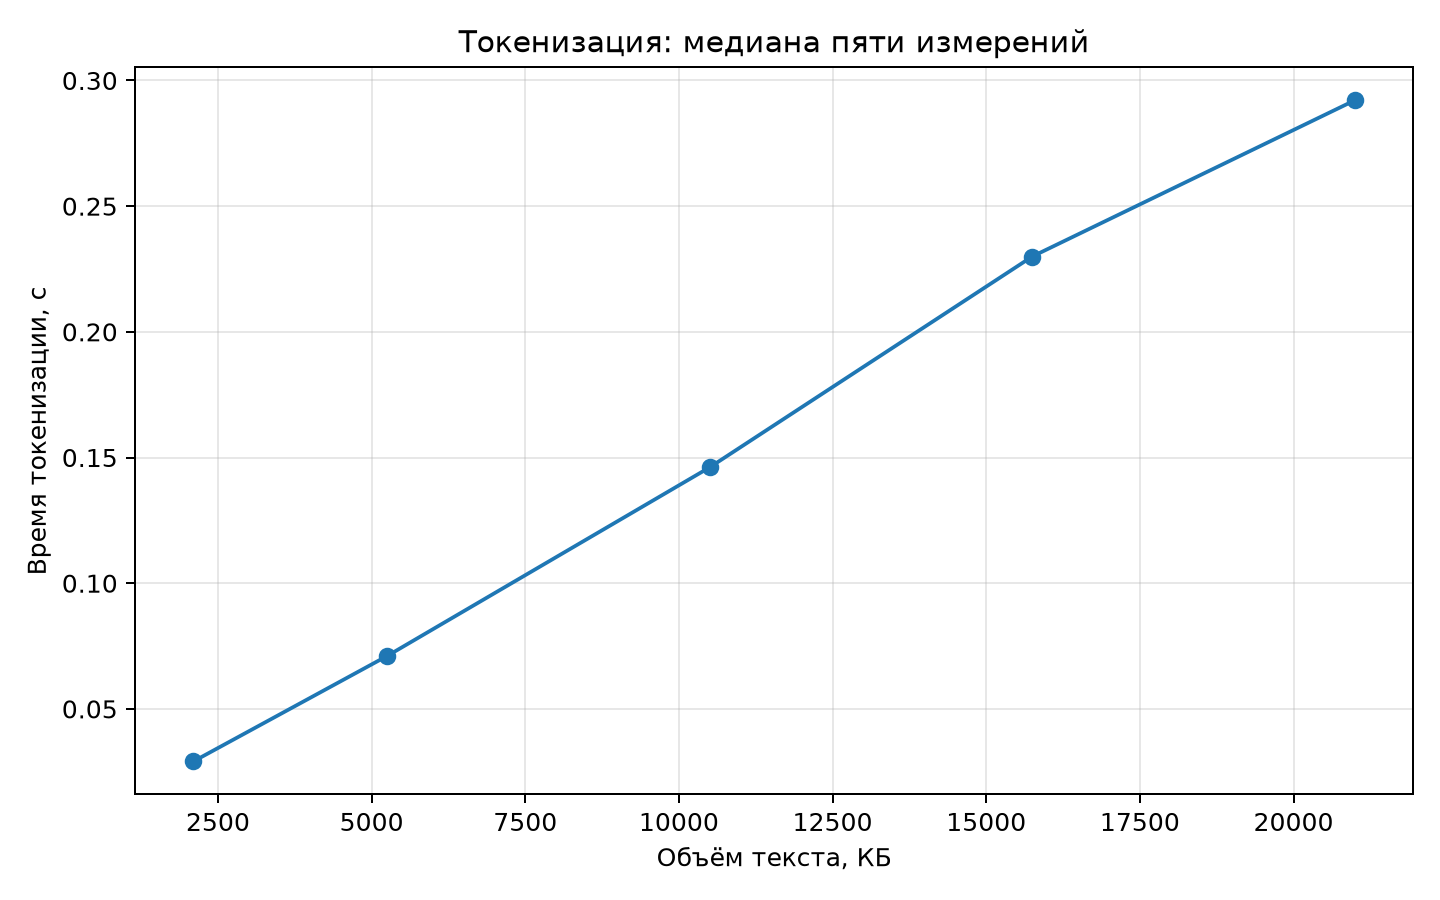
\includegraphics[width=0.94\linewidth]{lab03/results/time_vs_size.png}\caption{Время выделения токенов в зависимости от объёма входа}\end{figure}

Полный потоковый проход токенизации и стемминга занял 640,590 с, включая чтение и запись двух потоков. Скорость по чистому тексту: 8 191,02 КБ/с; 0,00012208 с/КБ. Это время двух этапов вместе; отдельный график выше измеряет только токенизатор на подвыборке, без файлового ввода-вывода.

\begin{figure}[H]\centering\begingroup
\sbox{\ScreenshotBox}{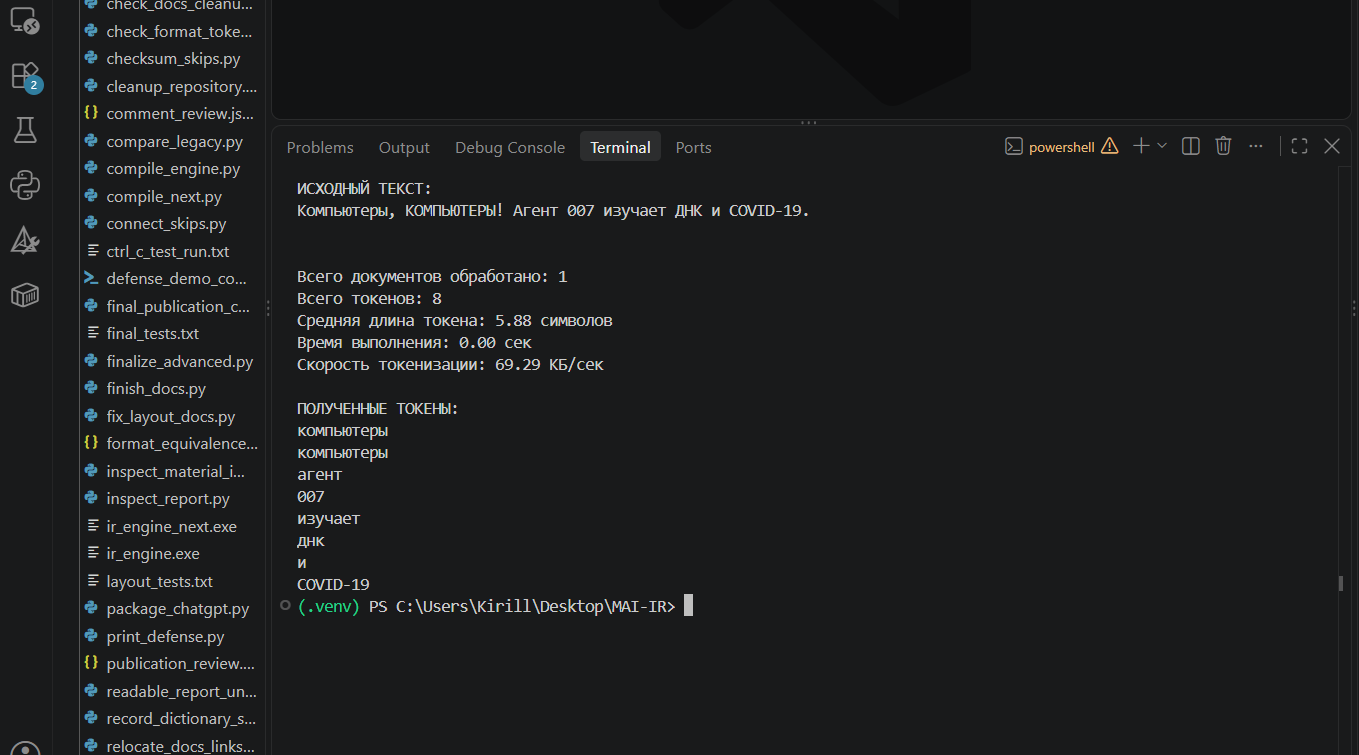
\includegraphics{images/screenshots/lab03_tokenization.png}}
\setlength{\ScreenshotLeft}{0.21339220\wd\ScreenshotBox}
\setlength{\ScreenshotBottom}{0.21192053\ht\ScreenshotBox}
\setlength{\ScreenshotRight}{0.37454010\wd\ScreenshotBox}
\setlength{\ScreenshotTop}{0.23178808\ht\ScreenshotBox}
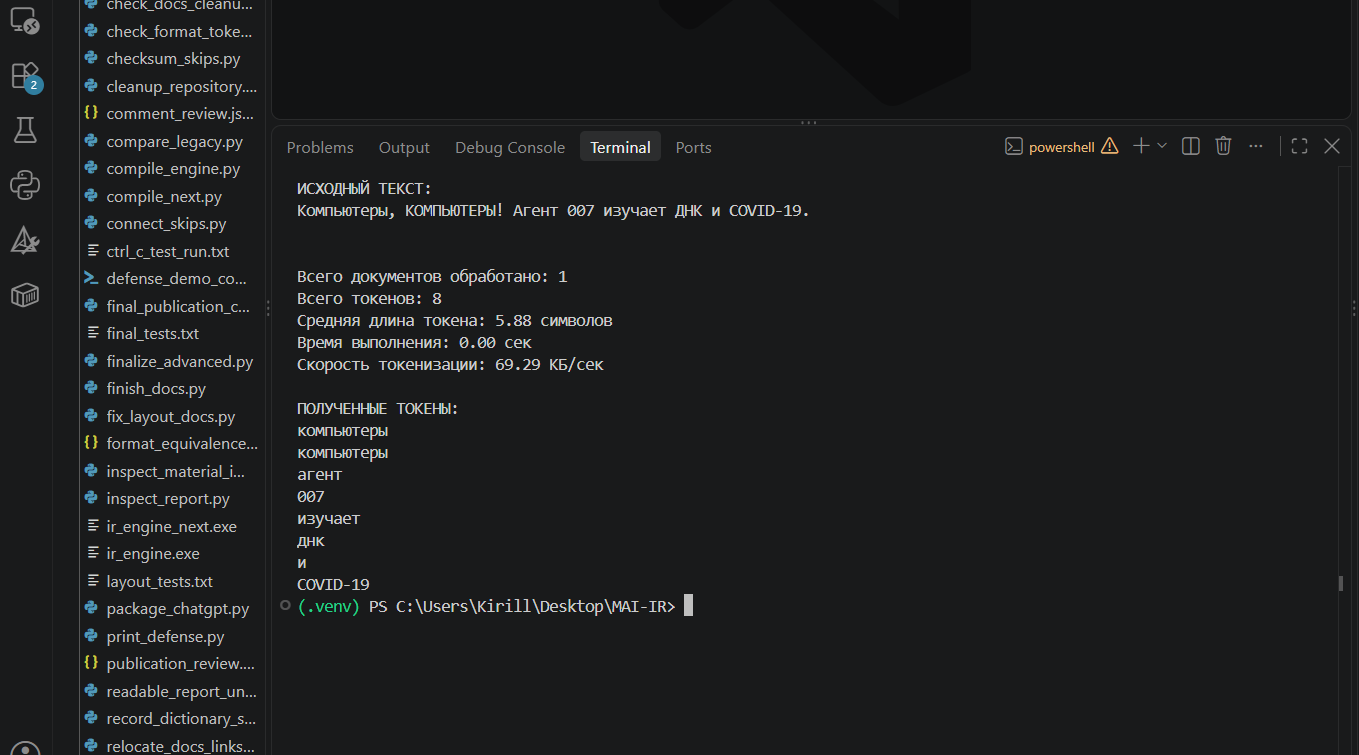
\includegraphics[trim={\ScreenshotLeft{} \ScreenshotBottom{} \ScreenshotRight{} \ScreenshotTop{}},clip,width=0.96\linewidth,height=0.70\textheight,keepaspectratio]{images/screenshots/lab03_tokenization.png}
\endgroup\caption{Пример токенизации и её статистика}\end{figure}


\sub{Выводы и ограничения}
Правила токенизации сохраняют полезные термины данного корпуса и применяются также к запросам. Полная Unicode-сегментация, распознавание химических формул и морфология латинских слов не реализованы. Это границы выбранной модели токена.

\section{Лабораторная работа № 4\\«Стемминг»}
\sub{Задание и алгоритм}
Стемминг сокращает слово по правилам русского алгоритма Snowball. Это позволяет искать близкие словоформы через общую основу. Результат может не быть словарным словом: «чтение» и «чтения» дают «чтен», «клетка» и «клетки» --- «клетк».

Код \code{lab04/funcs/stemmer.cpp} выполняет правила в заданном порядке: выделение областей слова, обработку окончаний и заключительных суффиксов. Ё приводится к е; латинские и цифровые обозначения не обрезаются русскими суффиксами. Используются собственные буферы без STL. Пакетный режим загружает настройки один раз для всех документов.
\sub{Проверки}
Результаты сверены с официальным русским словарём Snowball: 49 785 входных слов и ожидаемых основ, без расхождений. Эталоны и их происхождение находятся в \code{tests_lr3_4/reference/}. Дополнительно проверены пустые и длинные строки, ё, возвратные окончания, границы областей и смешанные обозначения.
\sub{Статистика и выводы}
Стемминг уменьшает число разных терминов. Число вхождений при этом сохраняется, поскольку стоп-слова не удаляются. Ограничение метода: он может объединить разные слова или не объединить нужные формы. Например, «клеток» не сводится к «клетк» этим алгоритмом.
\sub{Поиск по токенам и основам}
Сравнивается AND-поиск по исходным токенам и основам на двух фиксированных пулах: 16 и 14 документов. В них соответственно 5 и 6 документов отмечены как релевантные. Разметка выполнена ИИ и не проверялась независимым экспертом. Поэтому полнота ниже относится к размеченному пулу, а не ко всему корпусу. Данные эксперимента: \code{lab04/results_snowball/metrics.json}.

\begin{figure}[H]\centering\begingroup
\sbox{\ScreenshotBox}{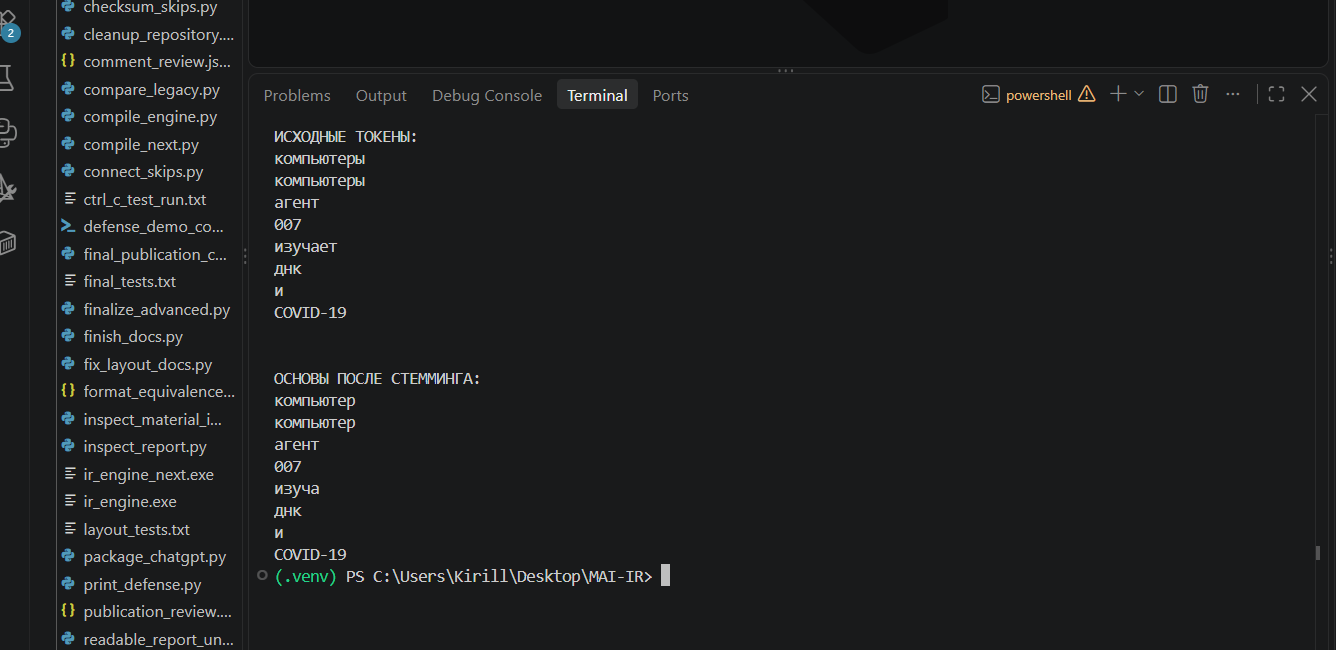
\includegraphics{images/screenshots/lab04_stemming.png}}
\setlength{\ScreenshotLeft}{0.19985030\wd\ScreenshotBox}
\setlength{\ScreenshotBottom}{0.13076923\ht\ScreenshotBox}
\setlength{\ScreenshotRight}{0.38622754\wd\ScreenshotBox}
\setlength{\ScreenshotTop}{0.19230769\ht\ScreenshotBox}
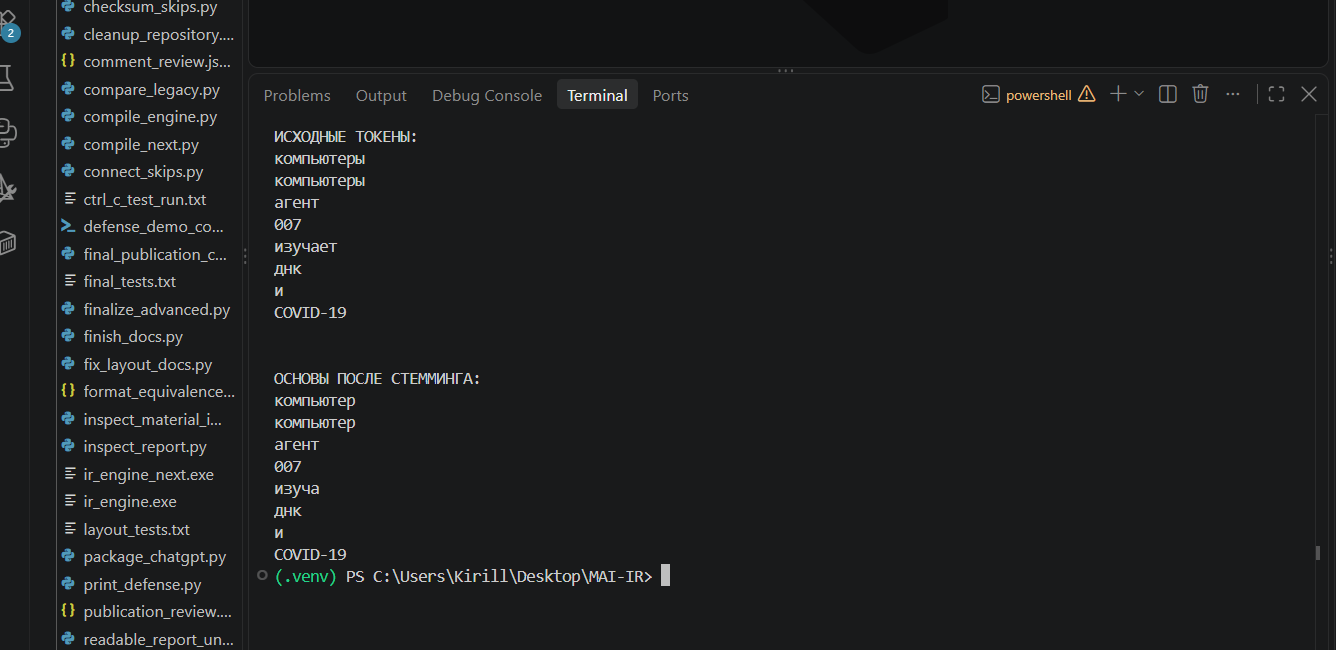
\includegraphics[trim={\ScreenshotLeft{} \ScreenshotBottom{} \ScreenshotRight{} \ScreenshotTop{}},clip,width=0.96\linewidth,height=0.70\textheight,keepaspectratio]{images/screenshots/lab04_stemming.png}
\endgroup\caption{Примеры словоформ и полученных основ}\end{figure}

\begin{table}[H]\centering\small
\caption{AND-поиск: фиксированные размеченные пулы до/после Snowball}
\begin{tabularx}{\linewidth}{|X|r|r|r|r|}\hline
Запрос / режим & Найдено & P & Полнота пула & F1 \\\hline
межпланетные корабли / токены & 5 & 0,400 & 0,400 & 0,400 \\\hline
межпланетные корабли / основы & 16 & 0,312 & 1,000 & 0,476 \\\hline
человекоподобные роботы / токены & 1 & 0,000 & 0,000 & 0,000 \\\hline
человекоподобные роботы / основы & 14 & 0,429 & 1,000 & 0,600 \\\hline
\end{tabularx}\end{table}


Для «межпланетных кораблей» полнота составляет 0,4 при поиске по токенам и 1 при поиске по основам; для «человекоподобных роботов» --- 0 и 1 соответственно. У первого запроса точность равна 0,4 и 0,3125 соответственно: поиск по основам находит больше документов, включая нерелевантные упоминания. Результат показывает пользу и ограничение морфологической нормализации на этих примерах.

\section{Лабораторная работа № 4\\«Словарная лемматизация»}
\sub{Метод и реализация}
Словарная лемматизация приводит словоформы к нормальной форме. Подготовка данных читает словоформы и парадигмы OpenCorpora,
а собственный C++ модуль ищет нормальную форму в собственной хеш-таблице. Готовый морфологический анализатор
в поиске не используется. Корпус и запрос обрабатываются одним словарём; неизвестный токен сохраняется.
Если у формы несколько лемм, выбирается первая по алфавиту после приведения ё к е.
Смысл по контексту не определяется: например, «стали» может относиться к стали или глаголу «стать».
Путь к словарю и контрольные суммы приведены в \code{data/morphology/provenance.json};
источник данных --- OpenCorpora, пакет \code{pymorphy3-dicts-ru}. Чтение словарных парадигм при подготовке
данных не подменяет C++ алгоритм нормализации. Программа: \code{src/ir/extensions.cpp}.
\sub{Результаты полного прохода}
\begin{table}[H]\centering\small
\caption{Словарная нормализация полного корпуса}
\begin{tabularx}{\linewidth}{|X|r|}\hline
Показатель & Значение \\\hline
Документов & 992 743 \\\hline
Вхождений лемм & 399 609 278 \\\hline
Изменённых вхождений & 193 864 085 \\\hline
Словоформ в словаре & 3 060 103 \\\hline
Уникальных лемм/сохранённых токенов индекса & 2 351 852 \\\hline
Время прохода, с & 380,167 \\\hline
\end{tabularx}\end{table}
\begin{table}[H]\centering\small
\caption{Расширенный поисковый набор: состав и размер}
\begin{tabularx}{\linewidth}{|X|r|}\hline
Часть & Размер, МБ \\\hline
Сжатый базовый индекс лемм & 819,058 \\\hline
Координатные списки & 3 327,027 \\\hline
Выбранная таблица прыжков & 243,082 \\\hline
Смещения исходных текстов & 7,942 \\\hline
Полный размер расширенного набора & 4 397,109 \\\hline
Словарные данные отдельно & 139,980 \\\hline
\end{tabularx}\end{table}
Общий размер расширенного поискового набора: 4,397 ГБ.\par
\sub{Диагностика качества и ограничения}
Использованы два фиксированных набора документов с ИИ-разметкой, без независимой человеческой проверки. Это ограниченная диагностика, не оценка всей коллекции. Кандидаты задаются явным OR; веса вычислены на полном корпусе, затем выдача фильтруется до размеченного набора.
\begin{table}[H]\centering\small
\caption{Сравнение стемминга и лемматизации на размеченных наборах}
\begin{tabularx}{\linewidth}{|X|r|r|r|}\hline
Запрос / режим & Точность & Полнота & NDCG@5 \\\hline
межпланетные корабли / stem & 0,312 & 1,000 & 0,723 \\\hline
человекоподобные роботы / stem & 0,429 & 1,000 & 0,345 \\\hline
межпланетные корабли / lemma & 0,312 & 1,000 & 0,723 \\\hline
человекоподобные роботы / lemma & 0,429 & 1,000 & 0,214 \\\hline
\end{tabularx}\end{table}
Возможные причины различий: нормализация словоформ, омонимия и изменение частот и норм. Эти факторы требуют отдельного анализа; улучшение любого запроса не гарантируется. Для уточнения нужны анализ контекста и независимая разметка.
\begin{figure}[H]\centering\begingroup
\sbox{\ScreenshotBox}{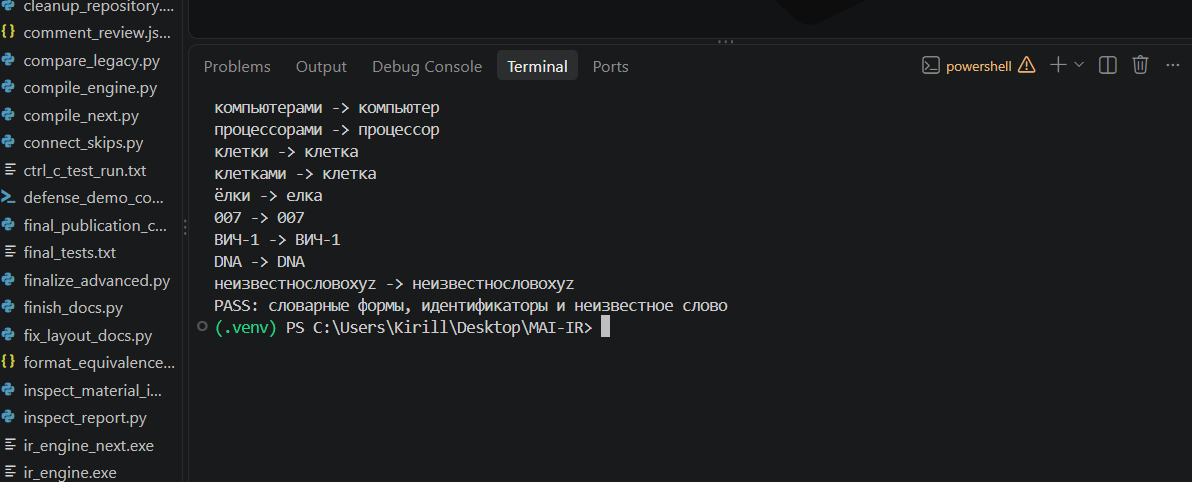
\includegraphics{images/screenshots/lab04_lemmatization.png}}
\setlength{\ScreenshotLeft}{0.17449664\wd\ScreenshotBox}
\setlength{\ScreenshotBottom}{0.34439834\ht\ScreenshotBox}
\setlength{\ScreenshotRight}{0.37080537\wd\ScreenshotBox}
\setlength{\ScreenshotTop}{0.19917012\ht\ScreenshotBox}
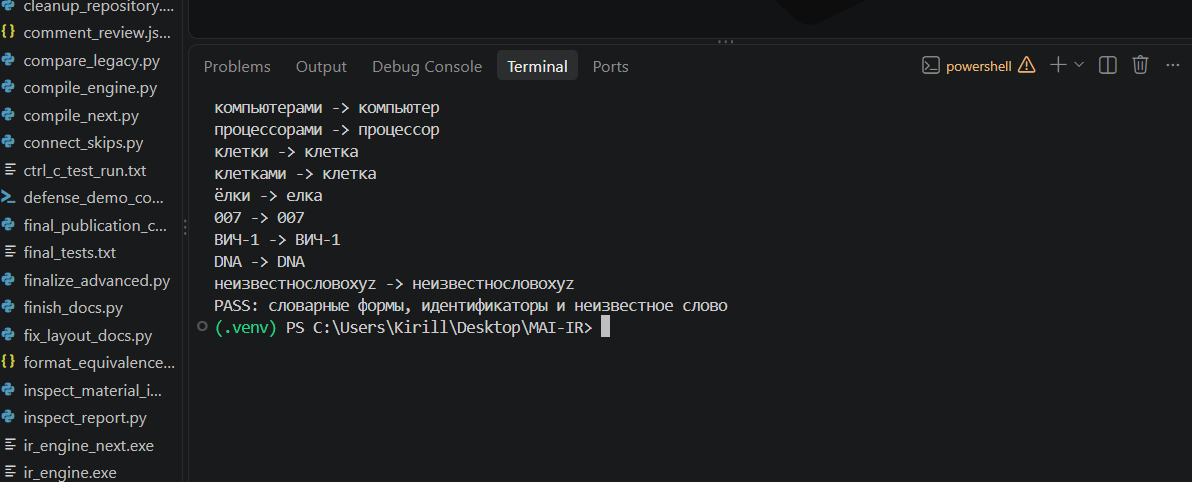
\includegraphics[trim={\ScreenshotLeft{} \ScreenshotBottom{} \ScreenshotRight{} \ScreenshotTop{}},clip,width=0.96\linewidth,height=0.70\textheight,keepaspectratio]{images/screenshots/lab04_lemmatization.png}
\endgroup\caption{Словарная лемматизация и её контрольные примеры}\end{figure}

\section{Лабораторная работа № 5\\«Закон Ципфа»}
\sub{Задание и реализация}
Закон Ципфа описывает частоты слов: небольшое число слов встречается очень часто, а большинство --- редко. График помогает проверить, похоже ли распределение собранного корпуса на распределение естественного текста.

Частоты считает \code{lab05/zipf_count.cpp}: собственная хеш-таблица накапливает все вхождения, сортировка слиянием упорядочивает термины по убыванию частоты. Python запускает счётчик и строит графики. Модель: $f(r)=f(1)/r$, где $r$ --- ранг, начиная с 1. На графике показаны первые 10 000 рангов; подсчёт выполнен для всего словаря. При равной частоте термины упорядочиваются по UTF-8.

\begin{figure}[H]\centering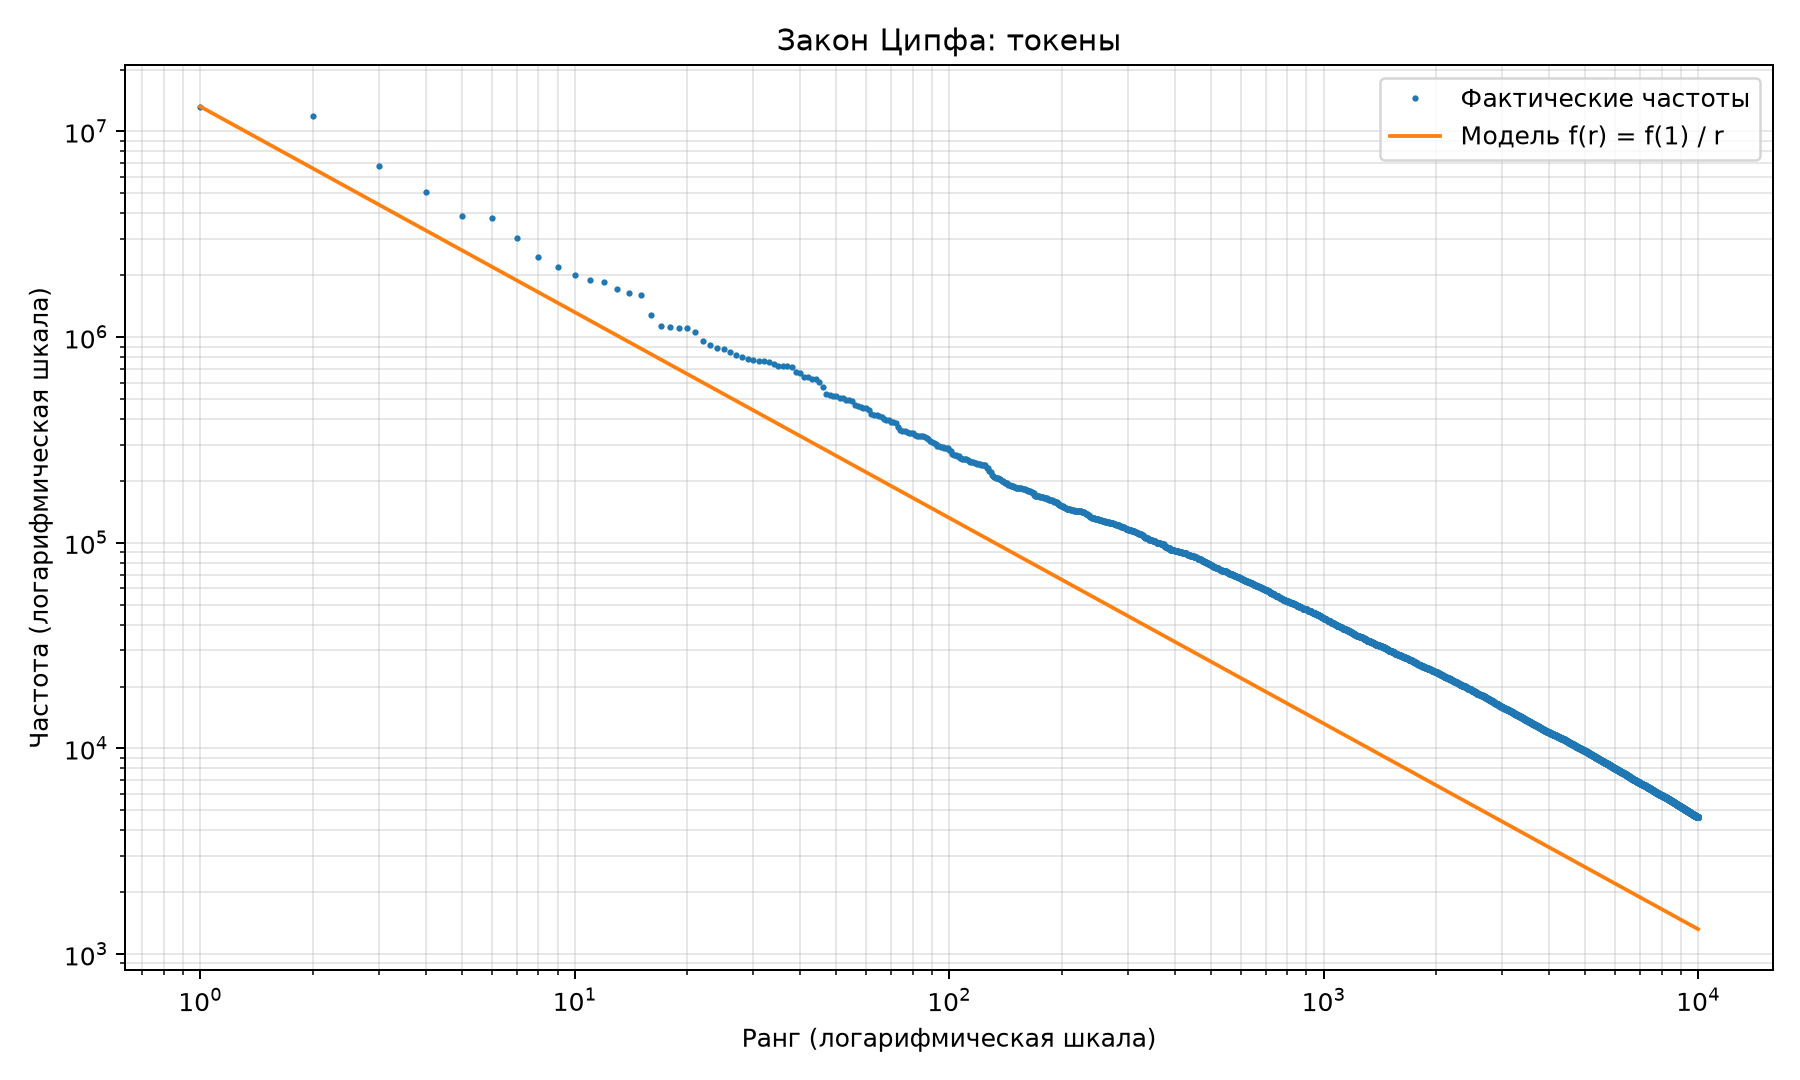
\includegraphics[width=0.94\linewidth]{lab05/results/tokens/zipf.png}\caption{Распределение токенов и модель Ципфа}\end{figure}

\begin{figure}[H]\centering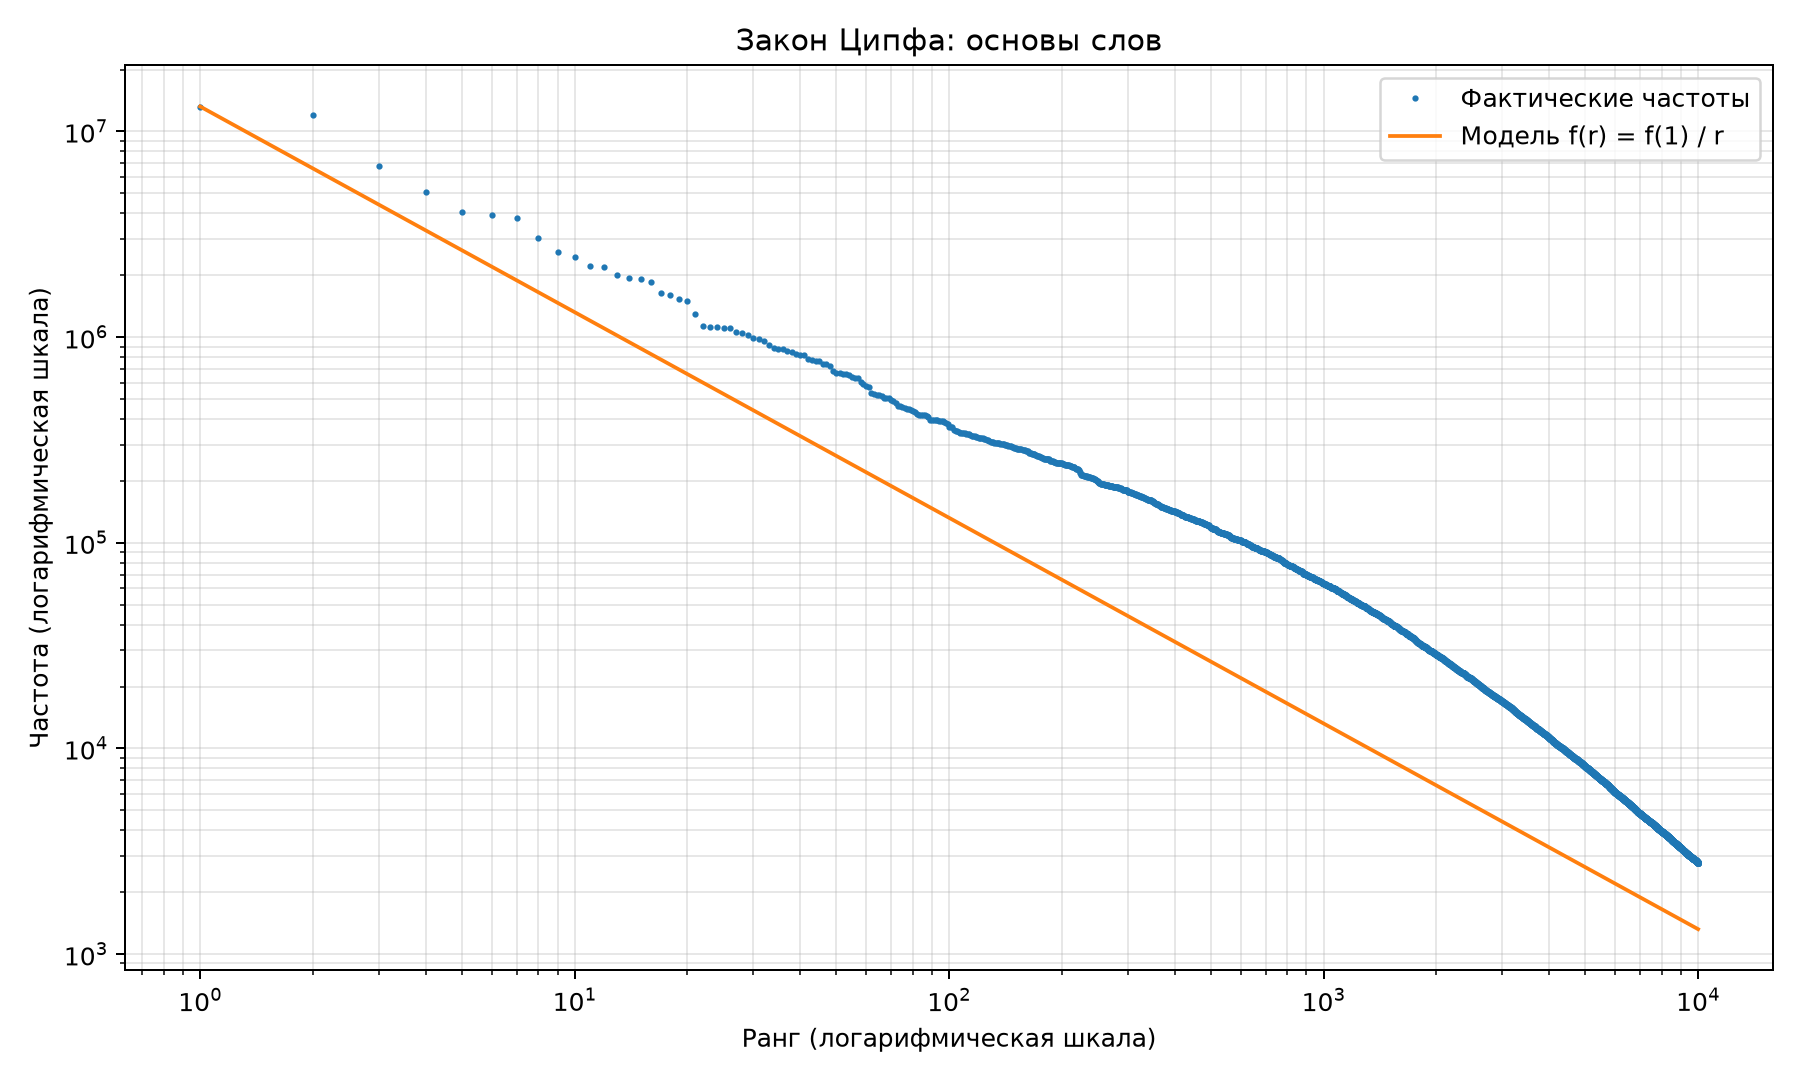
\includegraphics[width=0.94\linewidth]{lab05/results/stems/zipf.png}\caption{Распределение основ и модель Ципфа}\end{figure}


\sub{Выводы}
На графиках виден длинный хвост редких терминов. Реальные частоты отклоняются от модели: закон Ципфа описывает общую закономерность, а не точное значение для каждого слова. Тематика корпуса и объединение словоформ влияют на вид распределения.
\section{Лабораторная работа № 7\\«Булев индекс»}
\sub{Задание и структуры данных}
Обратный индекс сопоставляет каждому термину список документов, в которых он встретился. Элемент списка --- постинг: внутренний номер документа и частота термина в нём. Прямой индекс хранит исходный ID, заголовок, URL, длину и норму документа. Благодаря этому поиск не перечитывает весь корпус.

Реализация: \code{src/ir/engine.cpp}; собственные массивы, хеш-таблица, сортировка кучей и слияние серий находятся в \code{src/ir/base.h}. STL-контейнеры и готовые сортировщики в поисковом ядре не используются.

Документы обрабатываются по одному. Накопленные записи сортируются блоками, сохраняются во временные серии и затем сливаются. Параметр \code{--memory-mb 64} ограничивает полезный объём блока примерно 67,11 МБ. Он не задаёт предел всей памяти процесса: словарь, документы и резерв массивов учитываются отдельно.
\sub{Бинарный формат и надёжность}
Бинарный файл состоит из заголовка, прямого индекса, словаря терминов и списков постингов. Заголовок хранит версию, признаки формата и смещения секций. Числа записываются little-endian, строки --- в UTF-8 с длиной. Подробная схема: \code{src/ir/FORMAT.md}.

При чтении проверяются длины и смещения, версия, контрольная сумма, порядок docID и согласованность счётчиков. Готовый индекс публикуется после проверки временного файла.
\sub{План проверок и результаты}
Тестовый корпус содержит неупорядоченные внешние ID, повторения термина, пустой документ, UTF-8 метаданные и пути с пробелами. Проверяется построение в одном процессе и чтение в другом, восстановление tf/df и полного множества документов. Повреждённые и усечённые файлы должны отвергаться.

\begin{table}[H]\centering\small
\caption{Базовый несжатый индекс со стеммингом}
\begin{tabularx}{\linewidth}{|X|r|}\hline
Показатель & Значение \\\hline
Документов & 992 743 \\\hline
Терминов-основ & 1 963 565 \\\hline
Средняя длина уникального термина индекса, символов & 11,725 \\\hline
Средняя длина токена с учётом повторов, символов & 6,132 \\\hline
Постингов (пар термин–документ) & 216 715 451 \\\hline
Размер базового индекса, МБ & 2 053,111 \\\hline
Постинги, МБ & 1 733,724 \\\hline
Построение с процессом и проверкой, с & 310,297 \\\hline
Время на документ, мс & 0,3126 \\\hline
Время на КБ текста, мс & 0,05914 \\\hline
\end{tabularx}\end{table}

Средняя длина уникального термина и средняя длина токена с повторами считаются по-разному. Во втором случае частые слова имеют больший вес.

\begin{table}[H]\centering\small
\caption{Построение на подмножествах реальных документов}
\begin{tabularx}{\linewidth}{|X|r|r|}\hline
Документов & Время, с & Размер, МБ \\\hline
10 & 0,080 & 0,153 \\\hline
100 & 0,210 & 0,784 \\\hline
1 000 & 1,225 & 6,410 \\\hline
992 743 & 309,845 & 2 053,111 \\\hline
\end{tabularx}\end{table}

Подкорпусы состоят из первых уникальных документов снимка. Полная точка взята из основного построения. Разная длина статей влияет на время обработки.


\sub{Выводы и ограничения}
На реальных подмножествах измерены время и размер индекса. При дальнейшем увеличении корпуса растут словарь, число временных серий и объём слияния, поэтому время нельзя надёжно предсказать простым умножением.
\section{Лабораторная работа № 8\\«Булев поиск»}
\sub{Грамматика и исполнение}
CLI читает запросы по строке из stdin и возвращает JSONL в stdout. Пробел и \code{&&} означают И, \code{||} --- ИЛИ, \code{!} --- НЕ, поддержаны скобки и словесные AND/OR/NOT. Приоритет: НЕ, затем И, затем ИЛИ. Отрицание берётся относительно всех документов, включая пустые. Неизвестный термин соответствует пустому множеству. Пустой запрос возвращает пустую выдачу. Ошибка одной строки возвращает JSON с полем \code{error} и не останавливает обработку следующих строк.

Документы и запрос обрабатываются одинаковым нормализатором: в базовом режиме --- стеммером, в расширенном --- словарём лемм. Пересечение, объединение и разность выполняются над отсортированными массивами docID. Без ранжирования результаты упорядочены по внешнему ID как строки; этот порядок не отражает релевантность.
\sub{HTML-интерфейс}
\code{lab08/web.py} использует стандартный HTTP-сервер Python как обвязку C++-поиска. На начальной странице и странице результатов доступны форма и выбор TF-IDF; выводятся заголовки, URL, ID и по 50 результатов. Кнопки следующих/предыдущих 50 передают \code{--offset} ядру. HTML экранируется. Автоматические HTTP-тесты проверяют форму, поиск, страницы 50+6 результатов, отображение ошибок и метаданные. Сервис запускается локально командой \code{python lab08/web.py}, адрес \url{http://127.0.0.1:8080}.
\sub{Проверка правильности и времени}
Независимый эталон строится стандартными множествами в Python только в тестах, не в поисковой системе. Проверены операции, приоритеты, двойное отрицание, 80 воспроизводимо сгенерированных выражений, неизвестные слова, ошибки и продолжение потока. На настоящем корпусе исполняется пакет простых и сложных запросов; полные результаты сравниваются между бинарным и сжатым индексами.

\begin{table}[H]\centering\small
\caption{Поиск: медиана трёх пакетов запросов}
\begin{tabularx}{\linewidth}{|X|r|r|}\hline
Индекс / режим & Запросов & мс/запрос \\\hline
raw / булев & 23 & 923,837 \\\hline
raw / TF-IDF & 23 & 927,087 \\\hline
packed / булев & 23 & 846,113 \\\hline
packed / TF-IDF & 23 & 850,360 \\\hline
\end{tabularx}\end{table}


Приведённое время включает запуск процесса, загрузку индекса, пакет запросов и вывод до 50 результатов. Веб держит C++-процесс открытым: загрузка происходит при первом запросе, затем данные используются повторно. Для проверки сжатия полные выдачи исходного и сжатого индексов сравниваются отдельно по SHA-256.
\begin{figure}[H]\centering\begingroup
\sbox{\ScreenshotBox}{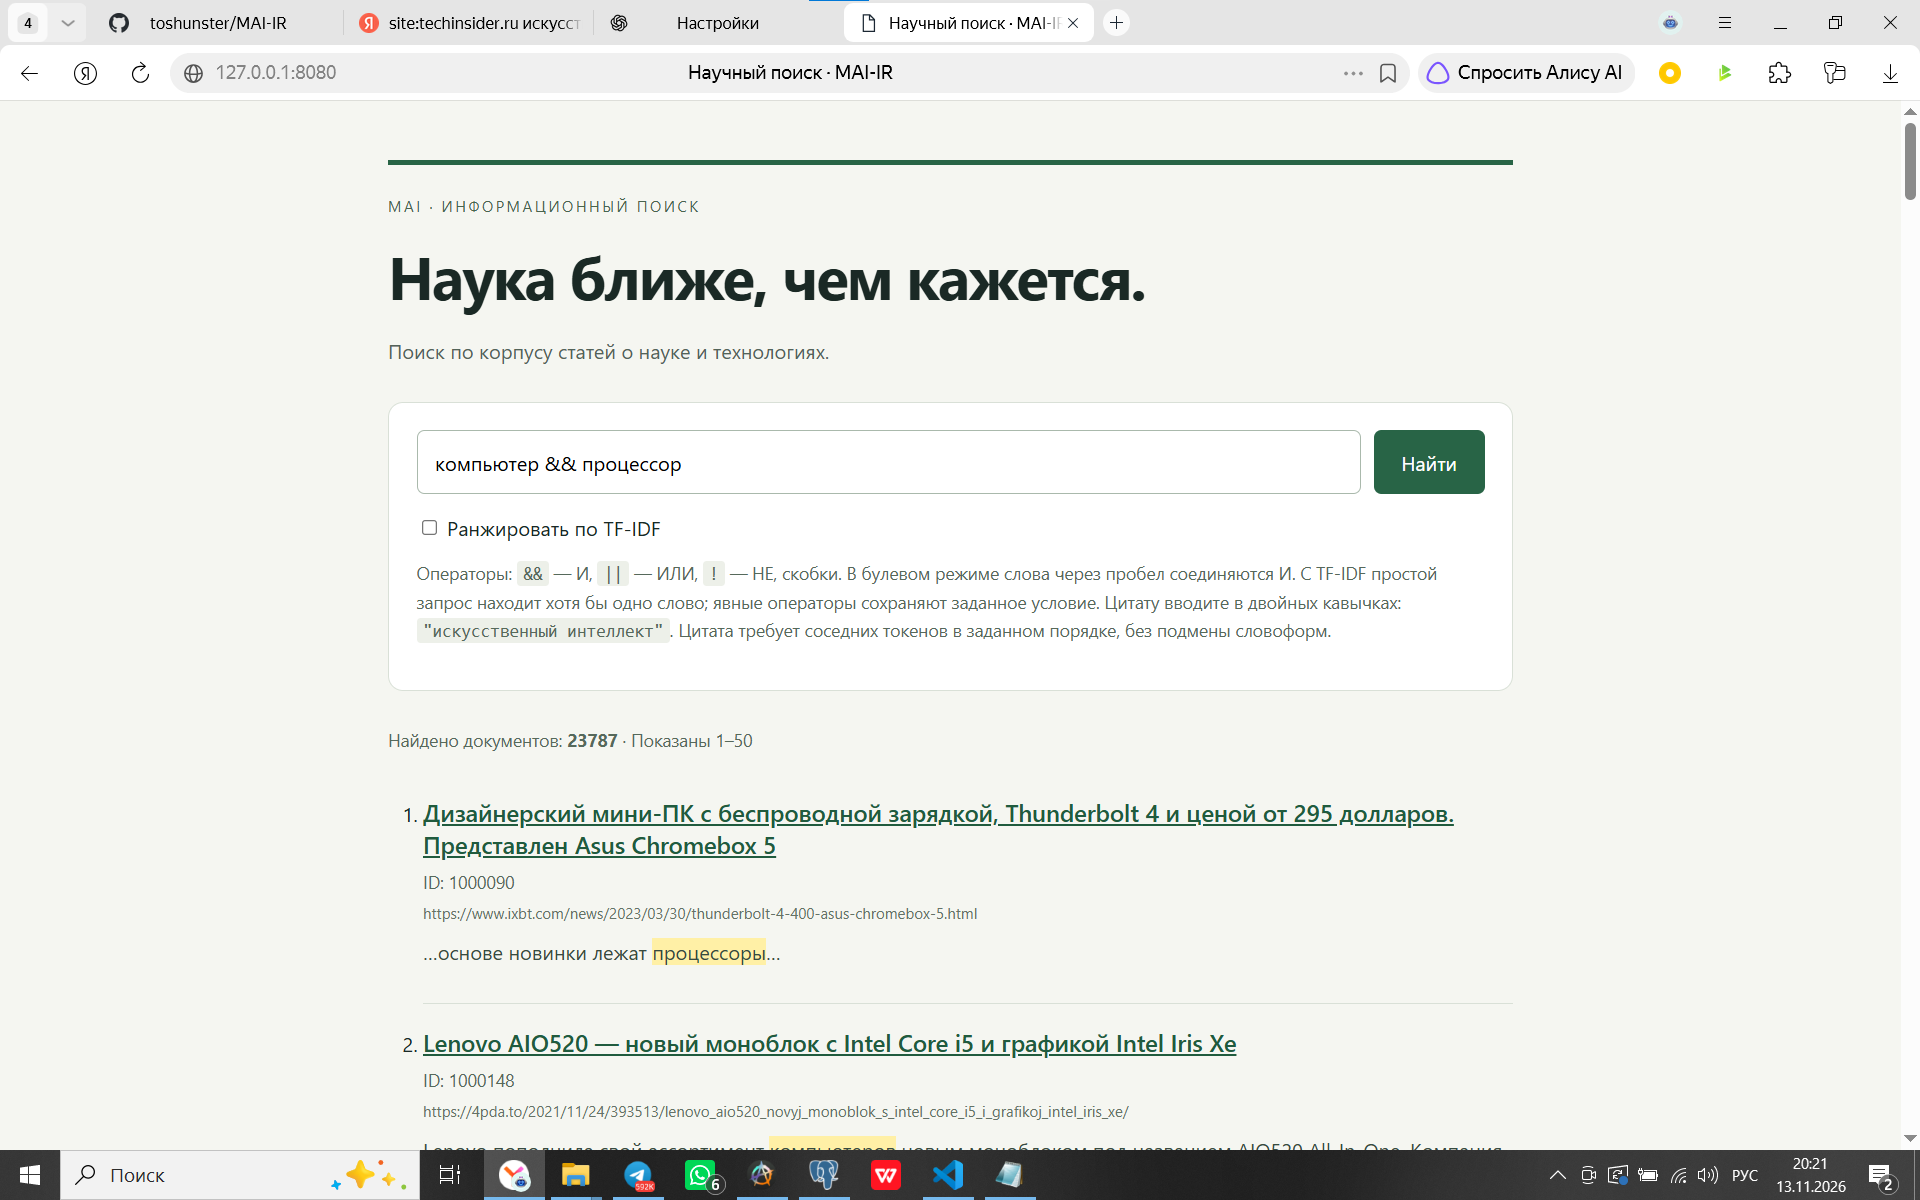
\includegraphics{images/screenshots/lab08_boolean.png}}
\setlength{\ScreenshotLeft}{0.20208333\wd\ScreenshotBox}
\setlength{\ScreenshotBottom}{0.16500000\ht\ScreenshotBox}
\setlength{\ScreenshotRight}{0.21093750\wd\ScreenshotBox}
\setlength{\ScreenshotTop}{0.33500000\ht\ScreenshotBox}
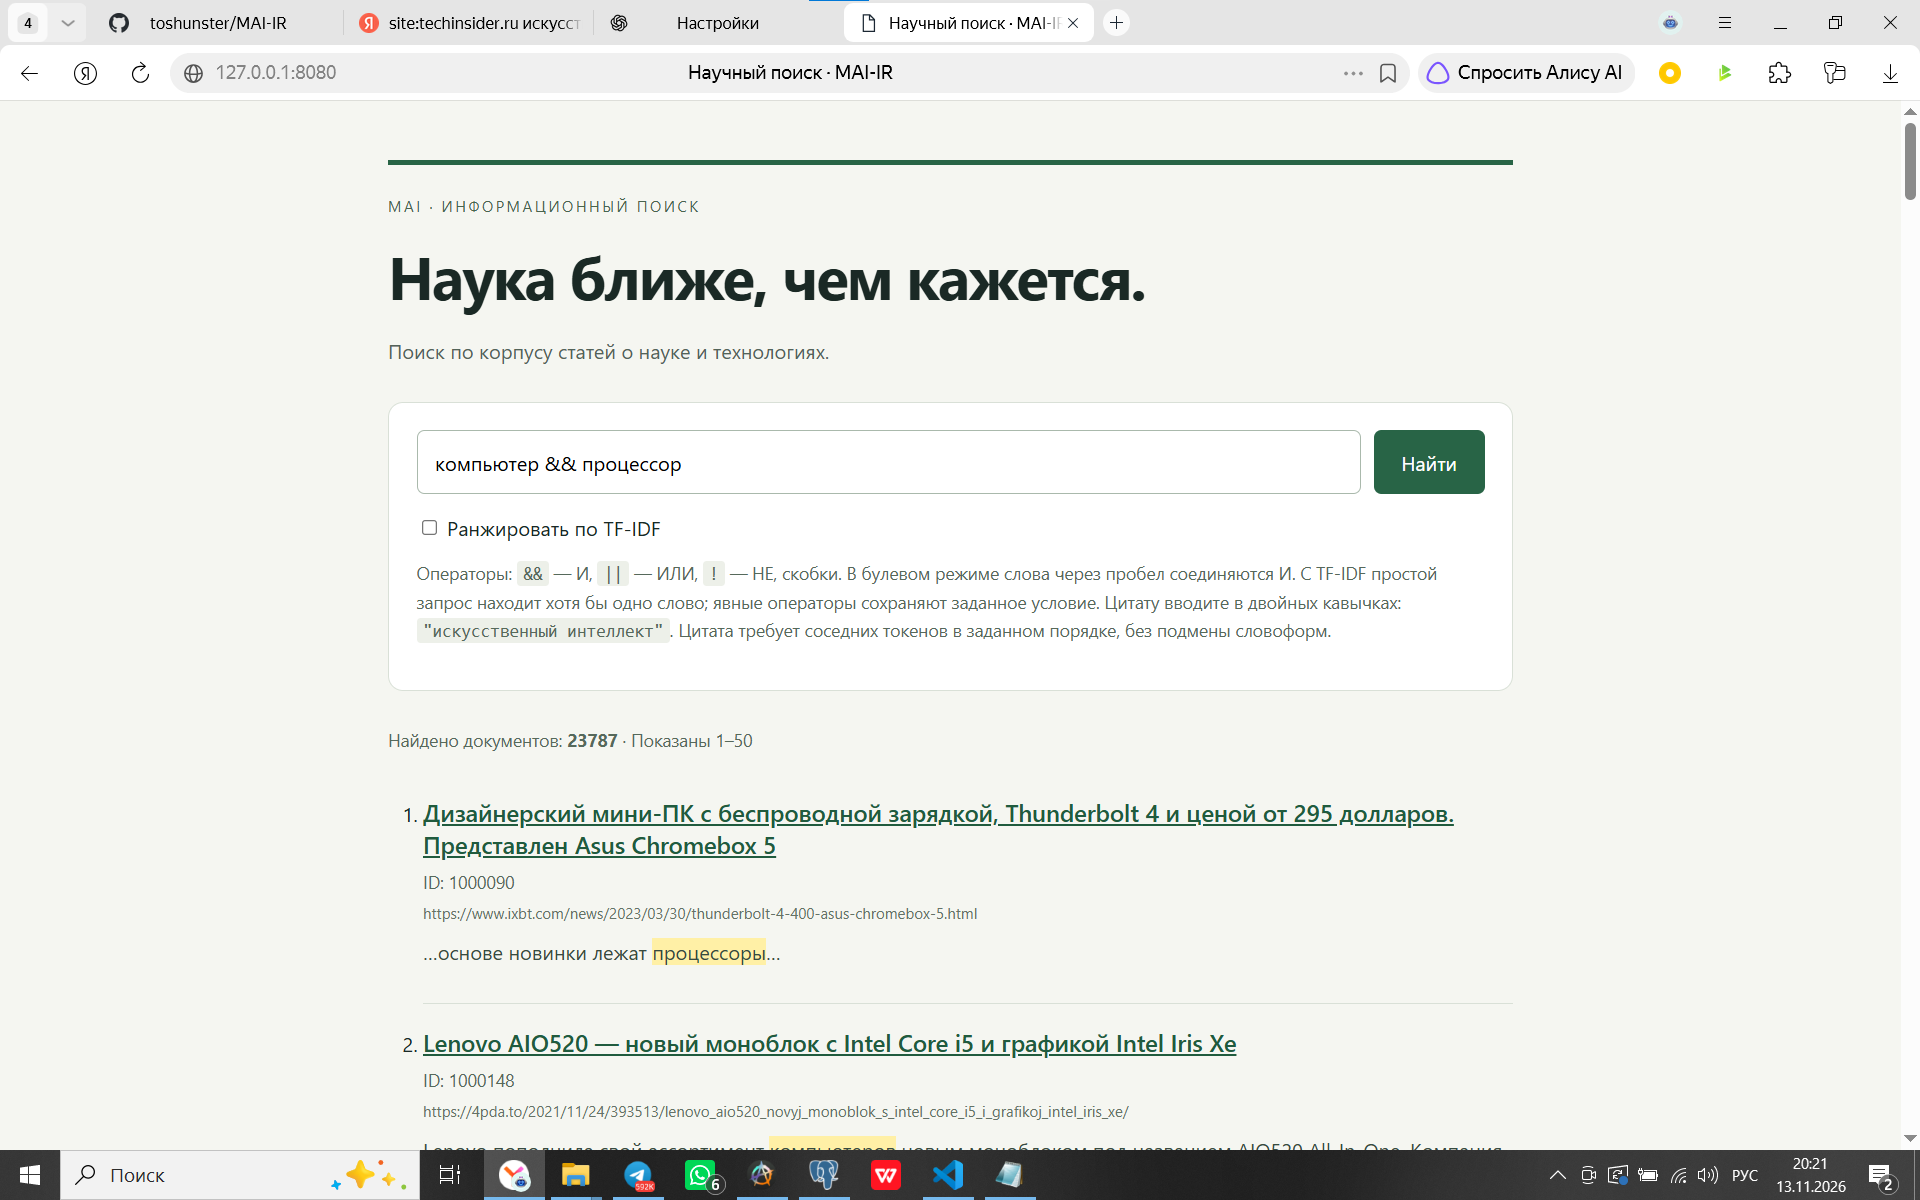
\includegraphics[trim={\ScreenshotLeft{} \ScreenshotBottom{} \ScreenshotRight{} \ScreenshotTop{}},clip,width=0.96\linewidth,height=0.70\textheight,keepaspectratio]{images/screenshots/lab08_boolean.png}
\endgroup\caption{Булева выдача по запросу «компьютер \&\& процессор»}\end{figure}


\section{Лабораторная работа № 10\\«Цитатный поиск и координаты»}
\sub{Строгое условие совпадения}
Двойные кавычки означают последовательность соседних исходных токенов в одном документе,
в заданном порядке. Регистр нормализуется, пунктуация разделяет токены, служебные слова сохраняются.
Словоформы внутри цитаты не заменяются леммами. Поэтому «кот дом» не совпадает с «кот большой дом»,
«дом кот» или отдельным «кот». Это строгое совпадение токенов, а не пунктуации исходного текста.
Цитата является узлом общего дерева AND/OR/NOT и фильтрует кандидатов до ранжирования.
\sub{Формат и построение}
Координатный индекс хранит для каждого исходного токена документы и позиции его вхождений.
Он строится внешней сортировкой в \code{positions.ir}.
Координата содержит 32 бита номера документа и 32 бита позиции. Заголовок 40 байт задаёт сигнатуру,
привязку к документам и количества; словарь хранит длину термина, его UTF-8 запись, начало и длину списка.
Каждая координата занимает 8 байт, little-endian. Списки k-го слова сдвигаются на k и пересекаются.
Перед вычитанием проверяется позиция: совпадение через границу документов исключено.
Координаты хранятся без сжатия; VB сжимает базовые пары doc/TF. Это ограничение текущей реализации.
\begin{table}[H]\centering\small
\caption{Координатный индекс}
\begin{tabularx}{\linewidth}{|X|r|}\hline
Показатель & Значение \\\hline
Документов & 992 743 \\\hline
Исходных терминов & 3 028 209 \\\hline
Координат & 399 609 278 \\\hline
Временных серий & 72 \\\hline
Среднее число координат на исходный термин & 131,962 \\\hline
Скорость по входному TSV, КБ/с & 12 419,102 \\\hline
Размер, МБ & 3 327,027 \\\hline
Построение, с & 430,971 \\\hline
\end{tabularx}\end{table}
Сравнены 46 полных выдач исходного и сжатого вариантов индекса. Для первых 50 результатов одной реальной цитаты независимо проверено наличие соседних токенов в исходных статьях. HTTP-проверки подтверждают вывод сниппетов и пустой ответ для цитаты с отсутствующим словом.
Независимый блочный аудит проверил все координаты: порядок, границы документов и позиций, итоговое количество. Пар «поверхностный термин–документ»: 256 583 876; среднее число позиций на такую пару: 1,557. Аудит не заменяет C++ поиск и читает только ограниченный блок готовых данных.
\begin{figure}[H]\centering\begingroup
\sbox{\ScreenshotBox}{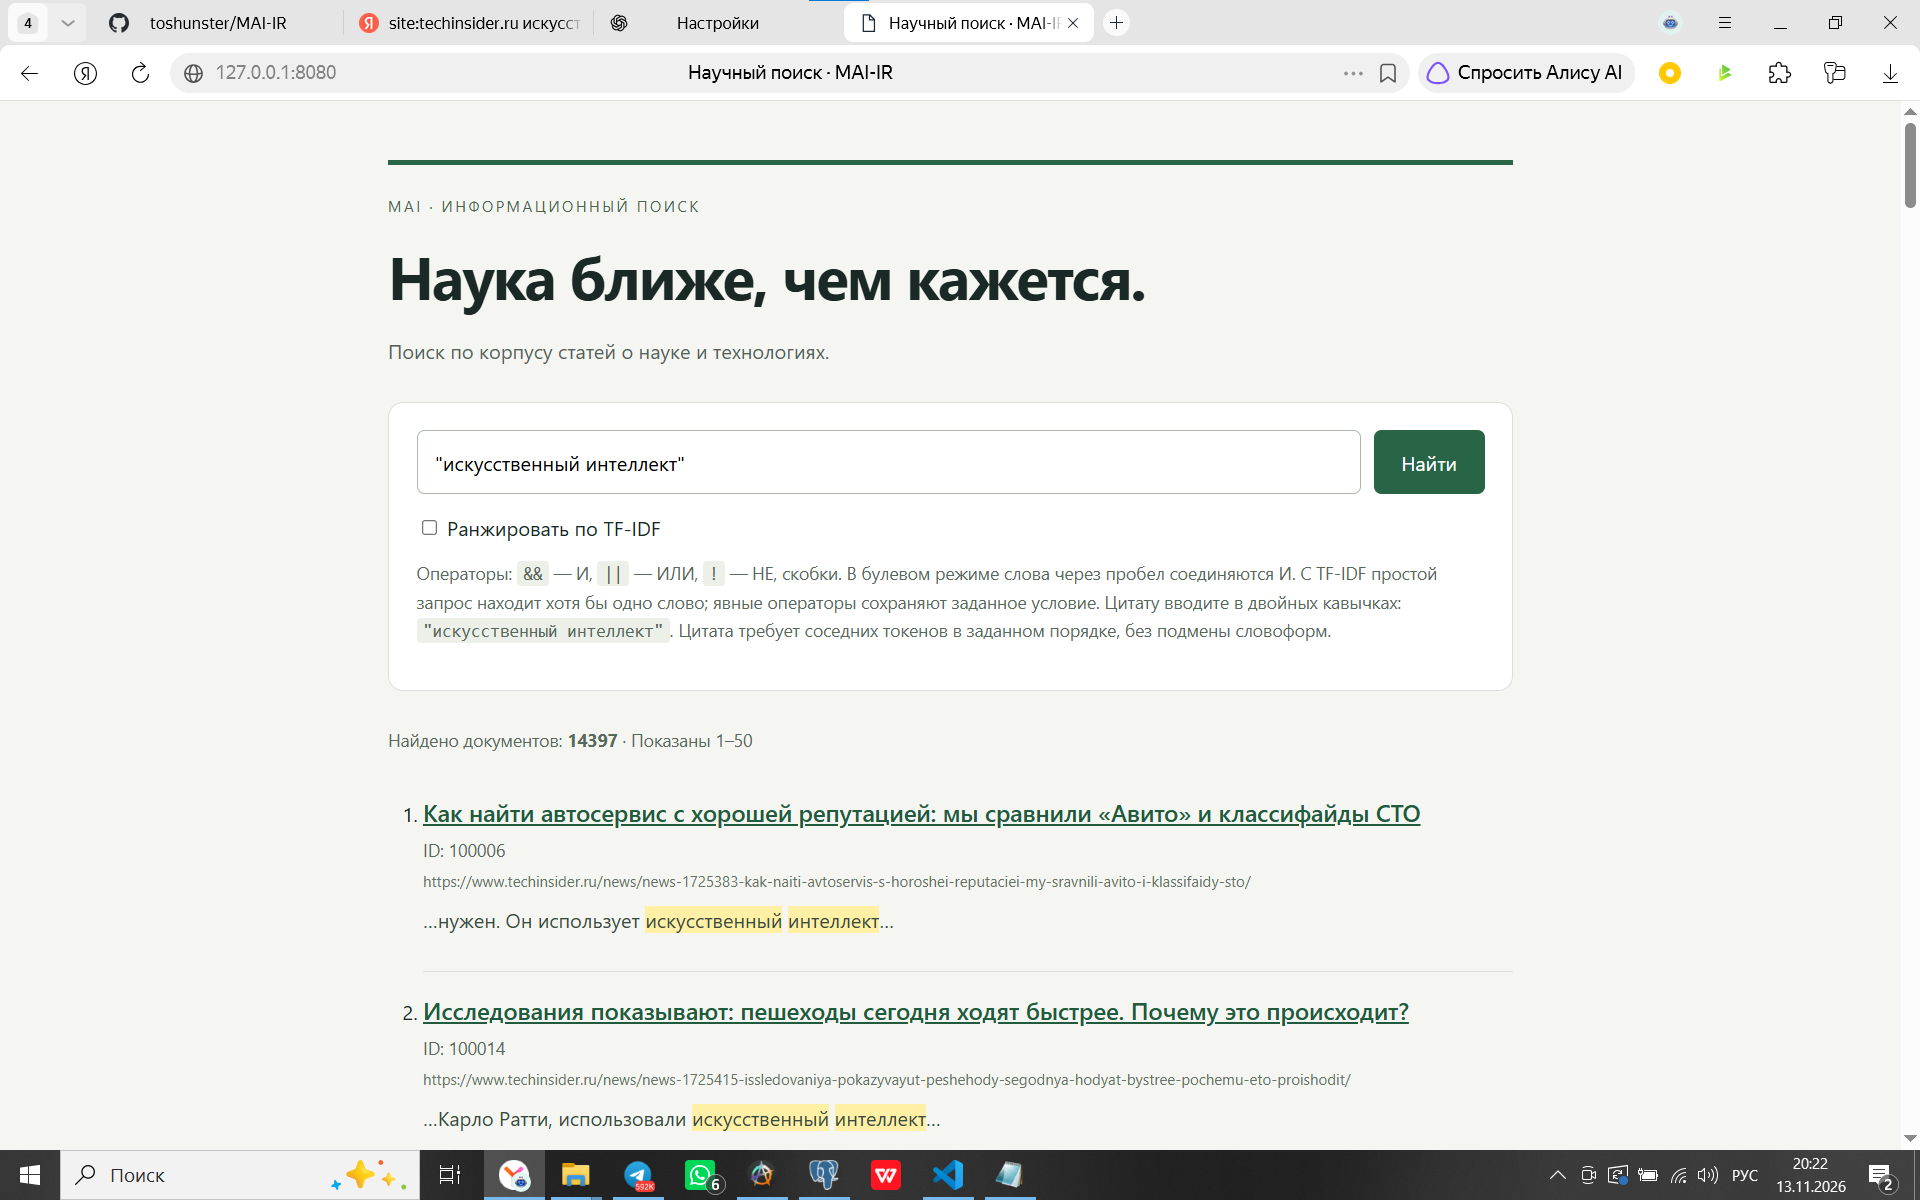
\includegraphics{images/screenshots/lab10_phrase.png}}
\setlength{\ScreenshotLeft}{0.20208333\wd\ScreenshotBox}
\setlength{\ScreenshotBottom}{0.05416667\ht\ScreenshotBox}
\setlength{\ScreenshotRight}{0.21093750\wd\ScreenshotBox}
\setlength{\ScreenshotTop}{0.33500000\ht\ScreenshotBox}
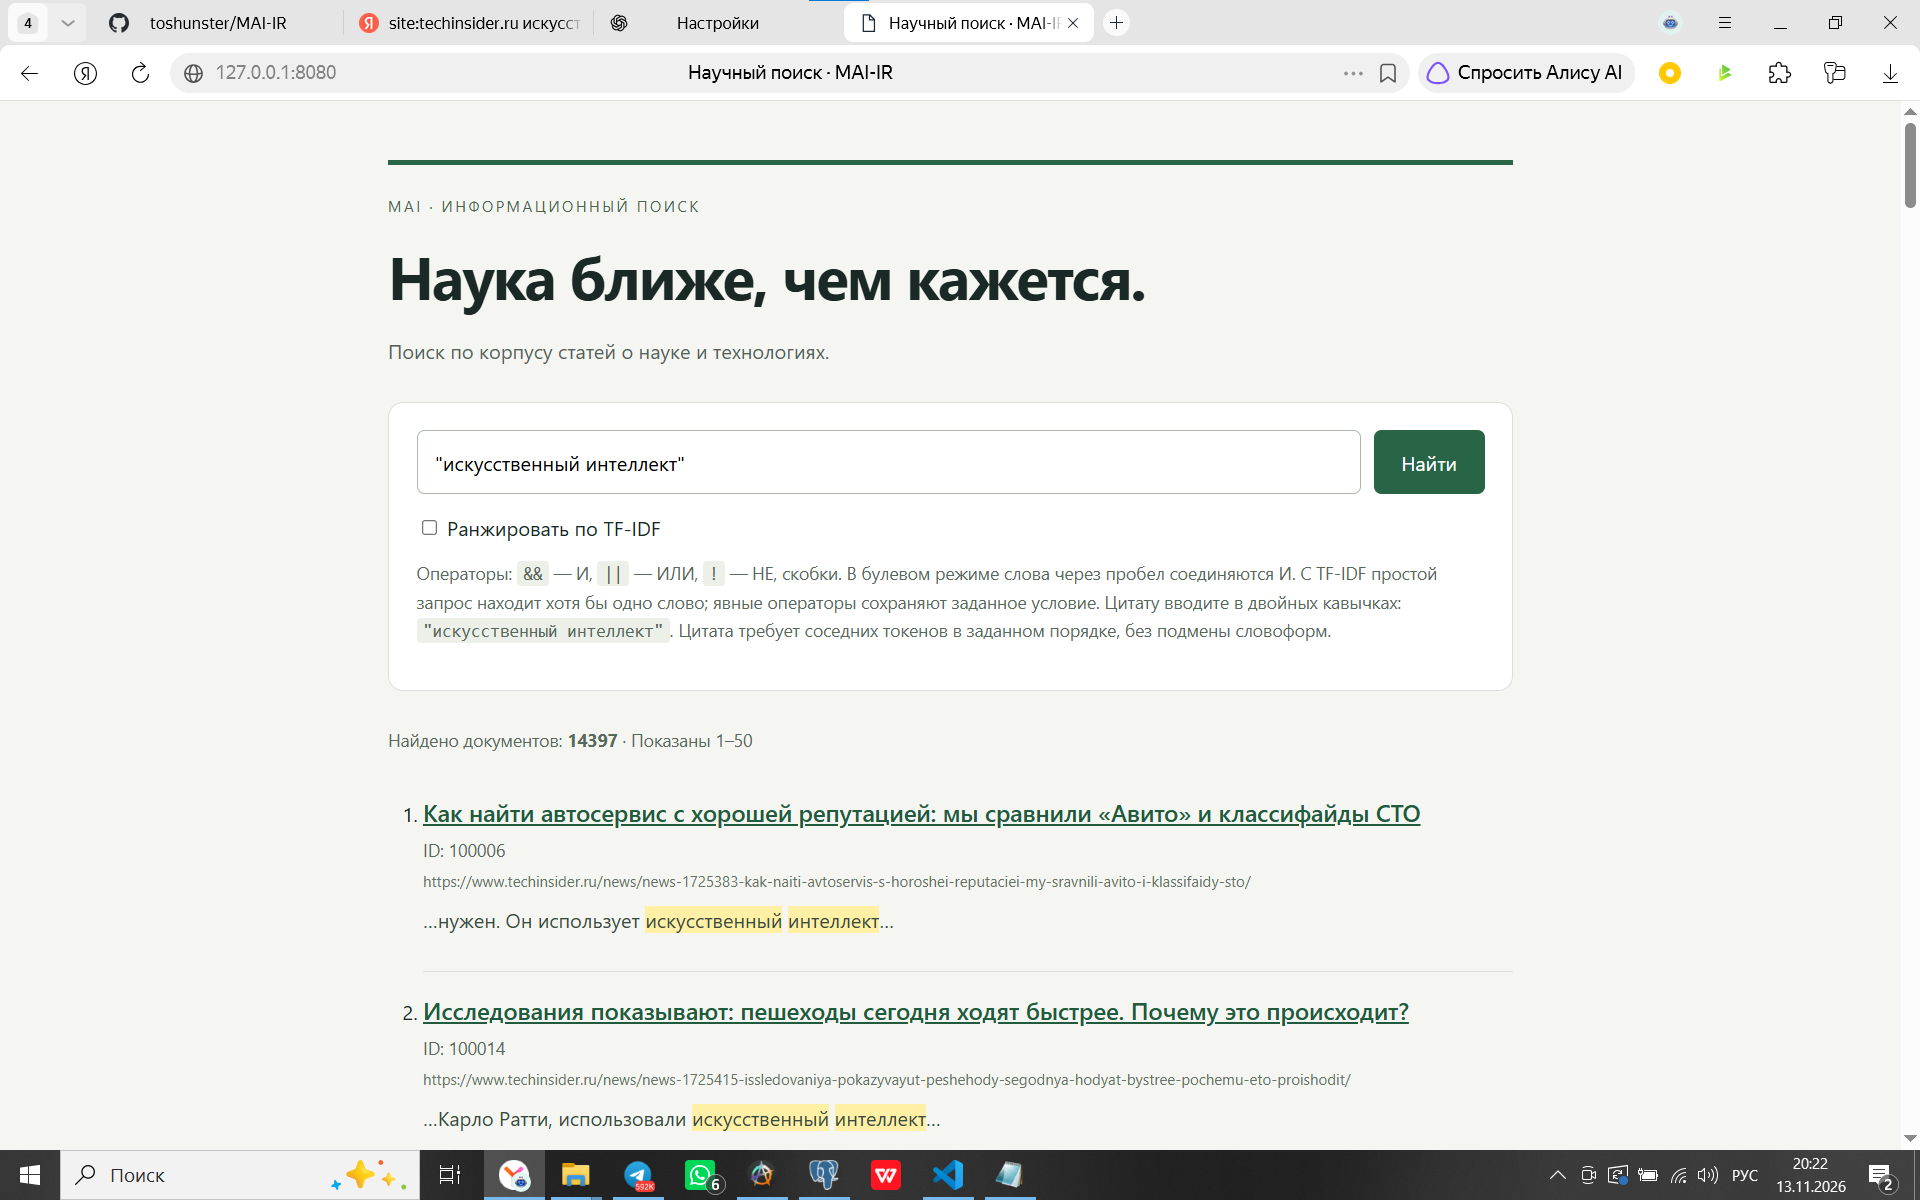
\includegraphics[trim={\ScreenshotLeft{} \ScreenshotBottom{} \ScreenshotRight{} \ScreenshotTop{}},clip,width=0.96\linewidth,height=0.70\textheight,keepaspectratio]{images/screenshots/lab10_phrase.png}
\endgroup\caption{Строгая цитата в веб-поиске}\end{figure}

\section{Лабораторная работа № 11\\«Сжатие индекса»}
\sub{Метод и формат}
В возрастающем списке docID первое число кодируется как $docID+1$, последующие --- как положительные промежутки. TF хранится отдельным целым. Используется Variable Byte: семь младших информационных бит на байт, группы идут от младших к старшим; старший бит последнего байта равен 1. Например, $0\mapsto\texttt{80}$, $127\mapsto\texttt{FF}$, $128\mapsto\texttt{00 81}$ (шестнадцатерично). Словарь, заголовки и URL остаются без сжатия. Несжатая база сравнения содержит пары 32-битных целых, а не заведомо невыгодный текстовый файл.

Метод выбран за простоту декодирования, побайтовое чтение и отсутствие потерь. Отвергаются переполнение, незавершённое число, лишние группы, невозможные интервалы и несогласованные длины. Проверяются границы 127/128, 16 383/16 384 и большие разрывы на отдельном синтетическом корпусе; этот корпус не включён в заявленное число настоящих статей.

\begin{table}[H]\centering\small
\caption{Сжатие: общий индекс и списки постингов}
\begin{tabularx}{\linewidth}{|X|r|r|}\hline
Часть & Без сжатия, МБ & Сжато, МБ \\\hline
Полный индекс & 2 053,111 & 797,375 \\\hline
Постинги & 1 733,724 & 477,988 \\\hline
Остальные секции & 319,387 & 319,387 \\\hline
\end{tabularx}\end{table}

Отношение полного сжатого размера к исходному: 0,3884. Время преобразования с проверкой: 108,837 с.

\begin{table}[H]\centering\small
\caption{Проход постингов: размеры (МБ) и медиана чтения/декодирования (мс)}
\begin{tabularx}{\linewidth}{|X|r|r|r|r|}\hline
Группа & raw, МБ & VB, МБ & raw, мс & VB, мс \\\hline
Редкие, df ≤ 2 & 13,672 & 6,708 & 2 054,025 & 2 051,152 \\\hline
Средние, 3 ≤ df ≤ 100 & 48,315 & 20,520 & 890,583 & 895,151 \\\hline
Частые, df > 100 & 1 671,737 & 450,759 & 4 789,481 & 4 440,271 \\\hline
Все блоки & 1 733,724 & 477,988 & 7 734,090 & 7 386,575 \\\hline
\end{tabularx}\end{table}


\sub{Проверки скорости и сохранения качества}
Отдельно измерены чтение и декодирование редких, средних и частых списков. Для выбранных запросов полностью совпали документы, порядок и баллы TF-IDF до и после сжатия. Значит, сжатие сохранило результат поиска. Измерения и контрольные суммы: \code{lab11/results/benchmark.json}.
\sub{Выводы}
Маленькие разности docID и частоты занимают меньше байтов. Общий выигрыш ограничен словарём и метаданными, которые остаются несжатыми. Скорость зависит от затрат на чтение и декодирование; результат приведён в таблице измерений.
\begin{figure}[H]\centering\begingroup
\sbox{\ScreenshotBox}{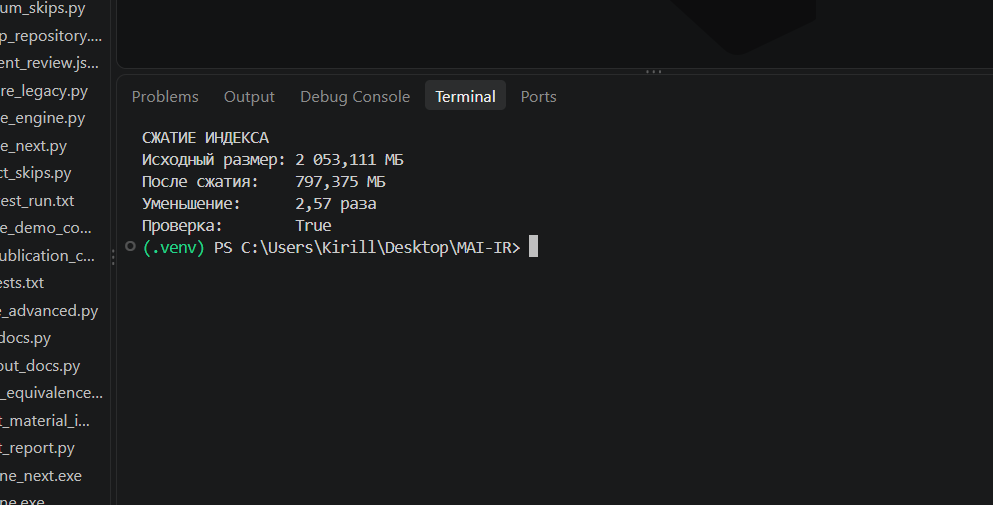
\includegraphics{images/screenshots/lab11_compression.png}}
\setlength{\ScreenshotLeft}{0.13695871\wd\ScreenshotBox}
\setlength{\ScreenshotBottom}{0.53465347\ht\ScreenshotBox}
\setlength{\ScreenshotRight}{0.50654582\wd\ScreenshotBox}
\setlength{\ScreenshotTop}{0.25148515\ht\ScreenshotBox}
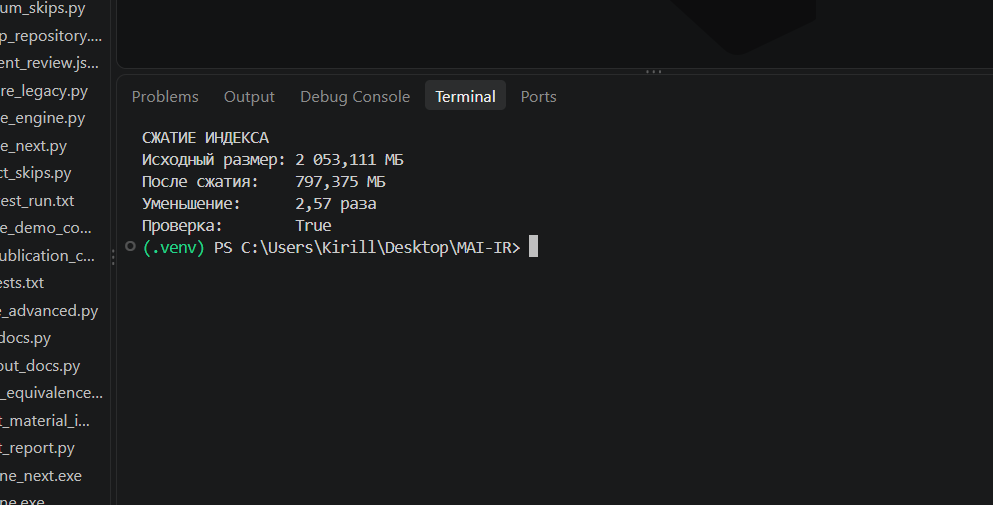
\includegraphics[trim={\ScreenshotLeft{} \ScreenshotBottom{} \ScreenshotRight{} \ScreenshotTop{}},clip,width=0.96\linewidth,height=0.70\textheight,keepaspectratio]{images/screenshots/lab11_compression.png}
\endgroup\caption{Проверка индекса и статистика сжатия}\end{figure}


\section{Лабораторная работа № 12\\«Прыжки по индексу»}
\sub{Метод и дополнительные поля}
Для длинных обратных списков сохраняется таблица точек перезапуска декодера. Каждая точка содержит
doc-ID, предыдущий doc-ID, порядковый номер постинга и байтовое смещение: четыре поля по 8 байт.
Предыдущий ID позволяет восстановить разности после прыжка. Таблица связана с контрольной суммой базового индекса.
Пересечение читает короткий список и ищет последнюю точку длинного списка, не превосходящую целевой ID.
Пропущенные постинги не декодируются. Списки короче 256 элементов обходятся обычным способом.
Специализация применяется к AND двух терминов; сложные подвыражения корректно вычисляются общим алгоритмом.
DF --- число документов с термином. Сравниваются фиксированные шаги и шаг по корню из DF.
\begin{table}[H]\centering\small
\caption{Выбор шага по обучающему пулу и проверка на другом пуле}
\begin{tabularx}{\linewidth}{|X|r|r|r|}\hline
Шаг & Размер, МБ & Обучение, мс & Проверка, мс \\\hline
32 & 243,082 & 22,817 & 11,334 \\\hline
128 & 89,434 & 23,849 & 12,301 \\\hline
корень из DF & 92,080 & 24,412 & 13,540 \\\hline
\end{tabularx}\end{table}
Выполнено пять измерений после прогревочного повторения. Время загрузки индекса исключено. Шаг выбирался только по обучающим запросам; второй пул не участвовал в выборе. Отношение времени без прыжков к времени выбранного варианта: на обучении 1,256, на проверке 1,543. Значение меньше единицы означает замедление, а не ускорение. Полные количества и первые 50 упорядоченных результатов совпали.
Сжатый блок читается один раз в буфер, прыжки пропускают декодирование, а не чтение диапазонов диска. Метаданные до 16 списков кешируются в пределах около 67,11 МБ. При слишком частых совпадениях стоимость выбора точки может превысить пользу пропуска. Поэтому результат зависит от соотношения длин списков и распределения ID; универсальное ускорение не обещается.
\begin{figure}[H]\centering\begingroup
\sbox{\ScreenshotBox}{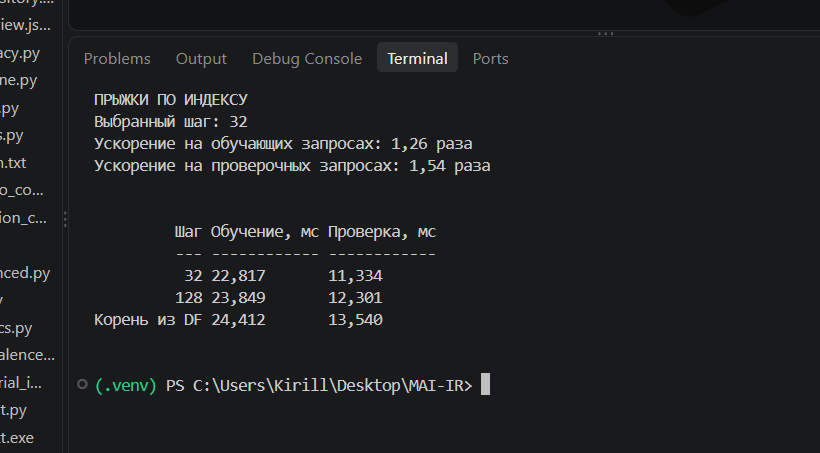
\includegraphics{images/screenshots/lab12_skips.png}}
\setlength{\ScreenshotLeft}{0.10731707\wd\ScreenshotBox}
\setlength{\ScreenshotBottom}{0.26490066\ht\ScreenshotBox}
\setlength{\ScreenshotRight}{0.32926829\wd\ScreenshotBox}
\setlength{\ScreenshotTop}{0.19646799\ht\ScreenshotBox}
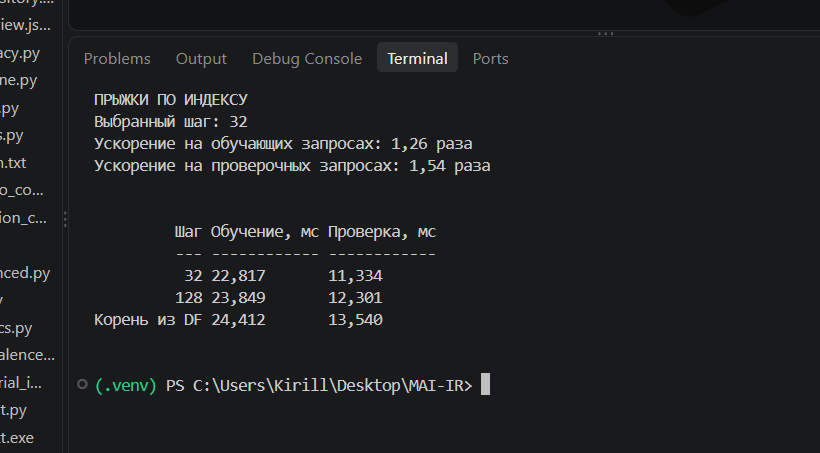
\includegraphics[trim={\ScreenshotLeft{} \ScreenshotBottom{} \ScreenshotRight{} \ScreenshotTop{}},clip,width=0.96\linewidth,height=0.70\textheight,keepaspectratio]{images/screenshots/lab12_skips.png}
\endgroup\caption{Измерения прыжков и сравнение с обычным пересечением}\end{figure}

\section{Лабораторная работа № 13\\«TF-IDF»}
\sub{Формула и семантика}
Пусть $N$ --- число документов, $df_t$ --- число документов с термином $t$, $tf_{t,d}$ --- число его вхождений. Принят сглаженный вариант IDF и логарифмический TF:
\[
\operatorname{idf}_t=\ln(1+N/df_t),\qquad
w_{t,d}=(1+\ln tf_{t,d})\operatorname{idf}_t,\quad tf_{t,d}>0.
\]
Отсутствующий термин имеет нулевой вес. Норма документа учитывает весь словарь, а не только слова текущего запроса. Запрос взвешивается так же с учётом повторов. Балл --- косинус:
\[
\operatorname{score}(q,d)=\frac{\sum_t w_{t,q}w_{t,d}}
{\sqrt{\sum_t w_{t,q}^2}\sqrt{\sum_t w_{t,d}^2}}.
\]
Сглаживание выбрано, чтобы термин во всех документах не получал нулевой IDF. Логарифм ослабляет влияние повторений, L2-норма --- влияние длины. Это конкретный вариант TF-IDF, а не единственная допустимая формула. Для нулевой нормы балл равен нулю, при равных баллах используется внешний ID.

Простой запрос из слов через пробелы использует OR-кандидатов. Наличие явного булева оператора включает строгое булево условие; затем совпадения ранжируются. Отрицательные ветви ограничивают множество документов и не добавляют положительного веса; двойное отрицание восстанавливает положительный вклад. Поэтому «клетки иммунитет» допускает неполное соответствие, а «клетки \&\& иммунитет» требует оба термина.
\sub{Проверки и оценка качества}
На малом корпусе TF, DF, IDF, полные L2-нормы и итоговые баллы рассчитаны независимыми формулами. Проверены редкие и частые термины, повторы в запросе, ничьи, отрицания и неизвестный термин. Оценка качества использует два запроса и 30 пар запрос--документ с ИИ-разметкой без независимой человеческой проверки. Для булевого и ранжированного режимов явно задаётся одинаковое OR-множество кандидатов. Поиск и веса вычисляются по полному индексу, затем результаты фильтруются до фиксированного размеченного пула каждого запроса. IDF и нормы не пересчитываются по маленькому пулу. Разметка фиксирована до вычисления метрик.

Ниже метрики диагностического пула при $k=5$: $P@k$ использует знаменатель $k$; $DCG=\sum(2^{rel}-1)/\log_2(i+1)$; NDCG делит DCG на идеальное значение; ERR использует бинарную шкалу и вероятность удовлетворения $(2^{rel}-1)/2$. Эти метрики характеризуют фиксированный размеченный пул, а не весь корпус. Для полной коллекции неизвестные оценки сохраняются неизвестными; охват и нижняя граница точности записаны отдельно в \code{lab13/results/quality.json}.

\begin{table}[H]\centering\small
\caption{Ограниченная оценка на фиксированном размеченном пуле, k=5}
\begin{tabularx}{\linewidth}{|X|r|r|r|r|}\hline
Запрос / режим & P@5 & DCG@5 & NDCG@5 & ERR@5 \\\hline
межпланетные корабли / ID & 0,600 & 1,931 & 0,655 & 0,615 \\\hline
межпланетные корабли / TF-IDF & 0,600 & 2,131 & 0,723 & 0,667 \\\hline
человекоподобные роботы / ID & 0,600 & 2,018 & 0,684 & 0,650 \\\hline
человекоподобные роботы / TF-IDF & 0,400 & 1,018 & 0,345 & 0,300 \\\hline
\end{tabularx}\end{table}

\begin{table}[H]\centering\small
\caption{Пример полного поиска: межпланетные корабли}
\begin{tabularx}{\linewidth}{|X|r|}\hline
ID / заголовок & TF-IDF \\\hline
58839 / NASA и SpaceX показали свои межпланетные ракеты. Главные новости науки сегодня & 0,53081 \\\hline
215803 / Илон Маск и колонизация Марса & 0,31266 \\\hline
198003 / Жизнь в космосе, или кто полетит на Марс? & 0,27775 \\\hline
51692 / Perseverance подтвердил, что в кратере Езеро было озеро. Главные новости за 14 сентября. & 0,26515 \\\hline
956004 / Дмитрий Рогозин рассказал, какими будут межпланетные космические станции и как будут их собирать & 0,26509 \\\hline
\end{tabularx}\end{table}

\begin{table}[H]\centering\small
\caption{Пример полного поиска: человекоподобные роботы}
\begin{tabularx}{\linewidth}{|X|r|}\hline
ID / заголовок & TF-IDF \\\hline
18809 / 10 необычных человекоподобных роботов & 0,44823 \\\hline
786900 / Китай поставит на учёт всех человекоподобных роботов & 0,44036 \\\hline
825720 / Overclockers.ru: Китайский автопроизводитель BYD в августе покажет своих первых человекоподобных роботов & 0,41734 \\\hline
639790 / Overclockers.ru: Продажи человекоподобных роботов в 2025 году составили 7000 единиц & 0,41513 \\\hline
336692 / «Аватар» в жизни: так выглядит модульный интерфейс для управления роботом & 0,40432 \\\hline
\end{tabularx}\end{table}

Запрос «межпланетные корабли»: NDCG@5 по фиксированному пулу составляет 0,655 в булевом режиме и 0,723 при ранжировании TF-IDF.

Запрос «человекоподобные роботы»: NDCG@5 по фиксированному пулу составляет 0,684 в булевом режиме и 0,345 при ранжировании TF-IDF.

\begin{figure}[H]\centering\begingroup
\sbox{\ScreenshotBox}{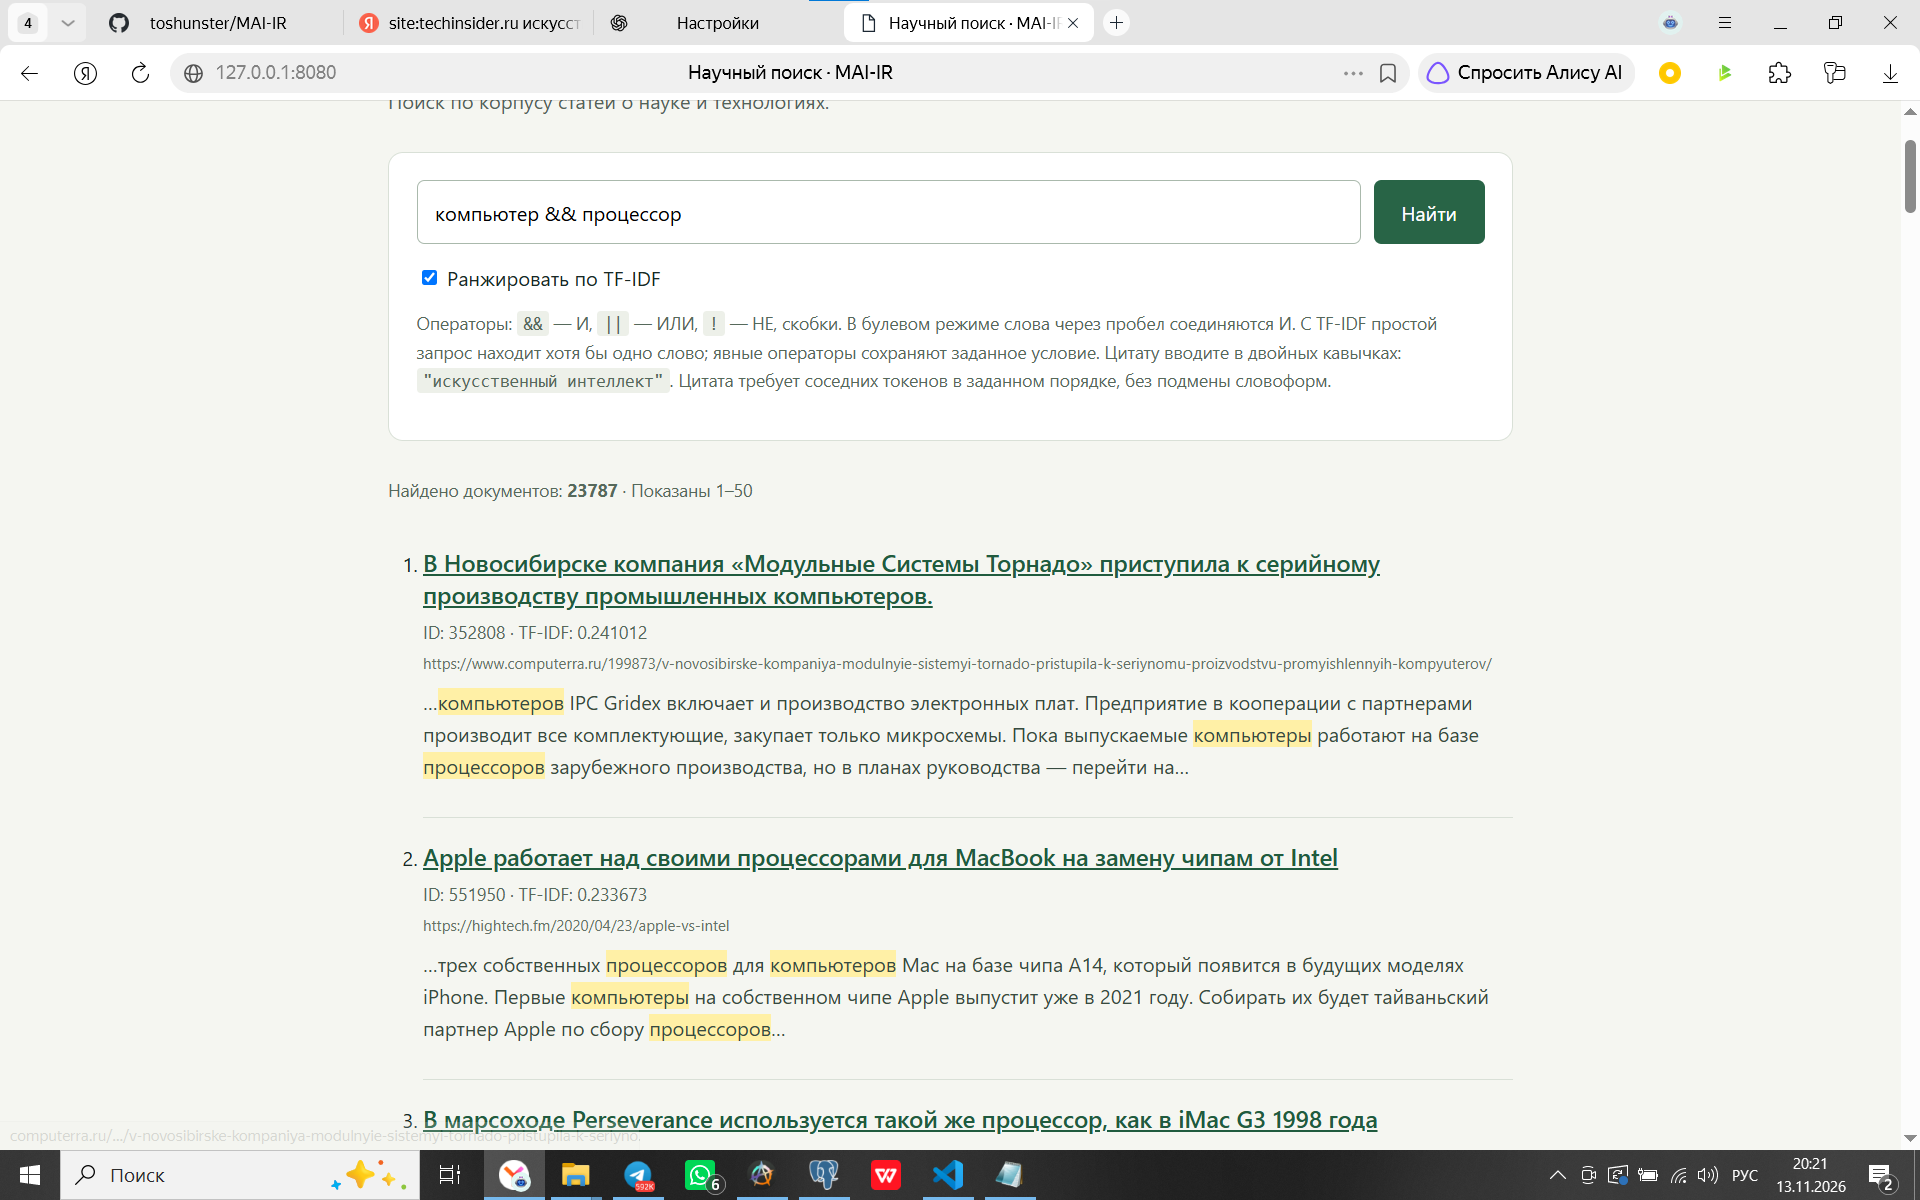
\includegraphics{images/screenshots/lab13_tfidf.png}}
\setlength{\ScreenshotLeft}{0.20208333\wd\ScreenshotBox}
\setlength{\ScreenshotBottom}{0.10000000\ht\ScreenshotBox}
\setlength{\ScreenshotRight}{0.21093750\wd\ScreenshotBox}
\setlength{\ScreenshotTop}{0.12750000\ht\ScreenshotBox}
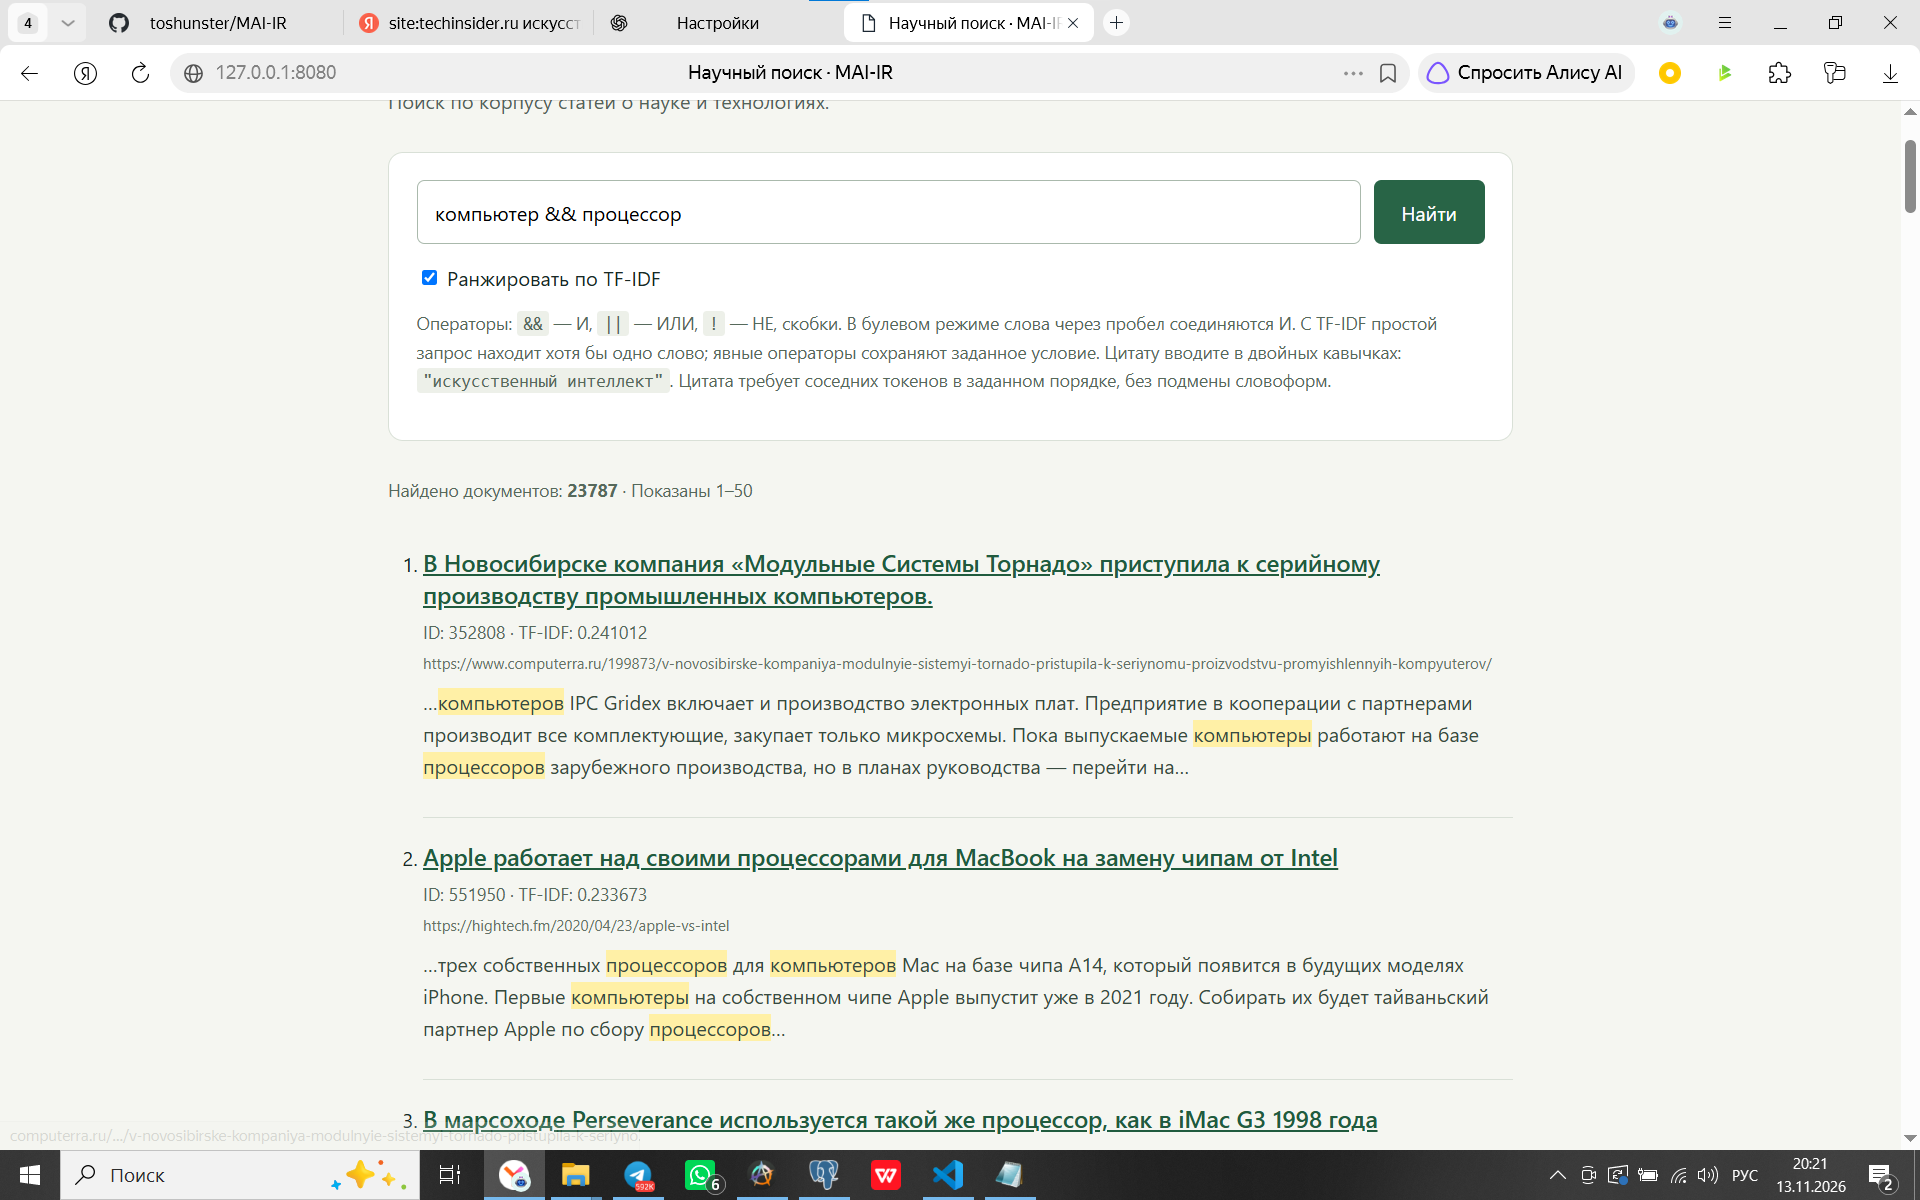
\includegraphics[trim={\ScreenshotLeft{} \ScreenshotBottom{} \ScreenshotRight{} \ScreenshotTop{}},clip,width=0.96\linewidth,height=0.70\textheight,keepaspectratio]{images/screenshots/lab13_tfidf.png}
\endgroup\caption{Пример ранжированной выдачи}\end{figure}


\sub{Выводы и ограничения}
TF-IDF ставит выше документы с более характерными словами запроса, но не понимает смысл текста. Случайные упоминания и многозначные слова могут дать нерелевантный результат. Метрики рассчитаны на двух пулах с ИИ-разметкой без независимой проверки и не характеризуют весь корпус. Ещё 18 примеров сохранены в \code{lab13/results/examples.json}.

\section{Лабораторная работа № 14\\«Построение сниппетов»}
Для документов текущей страницы выбирается окно до 36 токенов и 280 символов с наибольшим числом совпадений.
Исходная статья читается по таблице байтовых смещений, без повторного прохода по всему корпусу.
Совпадения определяются общей нормализацией запроса и документа, но выводится исходный текст со словоформами.
Отрицательные термины не подсвечиваются. Если положительных терминов нет, выводится начало статьи.
Обрезка контекста отмечается многоточием. C++ выдаёт части текста и признаки совпадения в JSON;
веб сначала экранирует каждую часть, затем добавляет собственную подсветку mark.
Это исключает исполнение HTML из статьи. Сниппет не меняет отбор или score.
Ограничения: окно не является смысловым рефератом, повтор одного слова может вытеснить более разнообразный контекст;
обрезка по 280 символам может прервать последнее слово; веб дополнительно ограничен тремя строками.
Если начало окна приближается к совпадению, его конец не расширяется: иногда контекста получается мало.
Тесты проверяют исходные словоформы, подсветку и экранирование опасного HTML.
\begin{figure}[H]\centering\begingroup
\sbox{\ScreenshotBox}{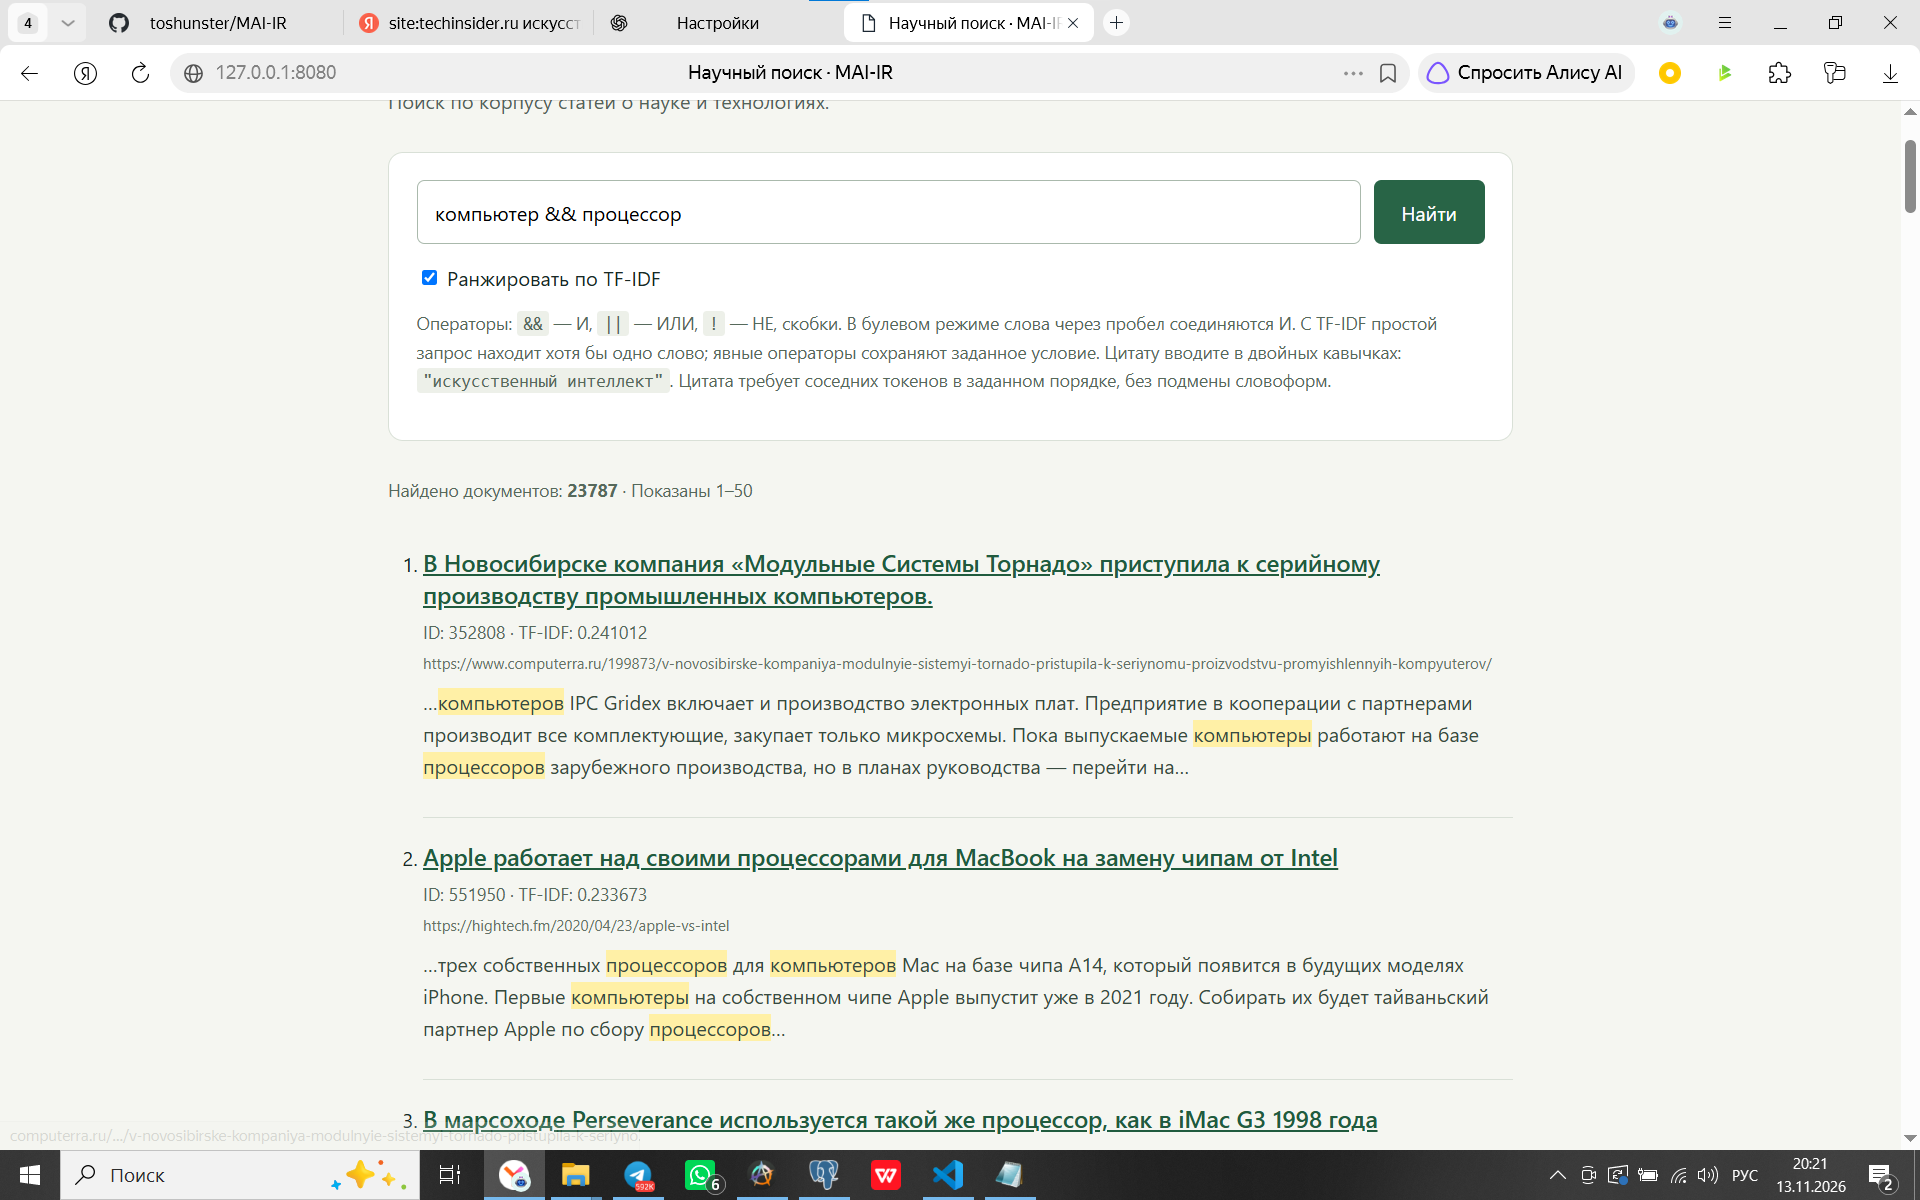
\includegraphics{images/screenshots/lab14_snippets.png}}
\setlength{\ScreenshotLeft}{0.21614583\wd\ScreenshotBox}
\setlength{\ScreenshotBottom}{0.12666667\ht\ScreenshotBox}
\setlength{\ScreenshotRight}{0.21093750\wd\ScreenshotBox}
\setlength{\ScreenshotTop}{0.45666667\ht\ScreenshotBox}
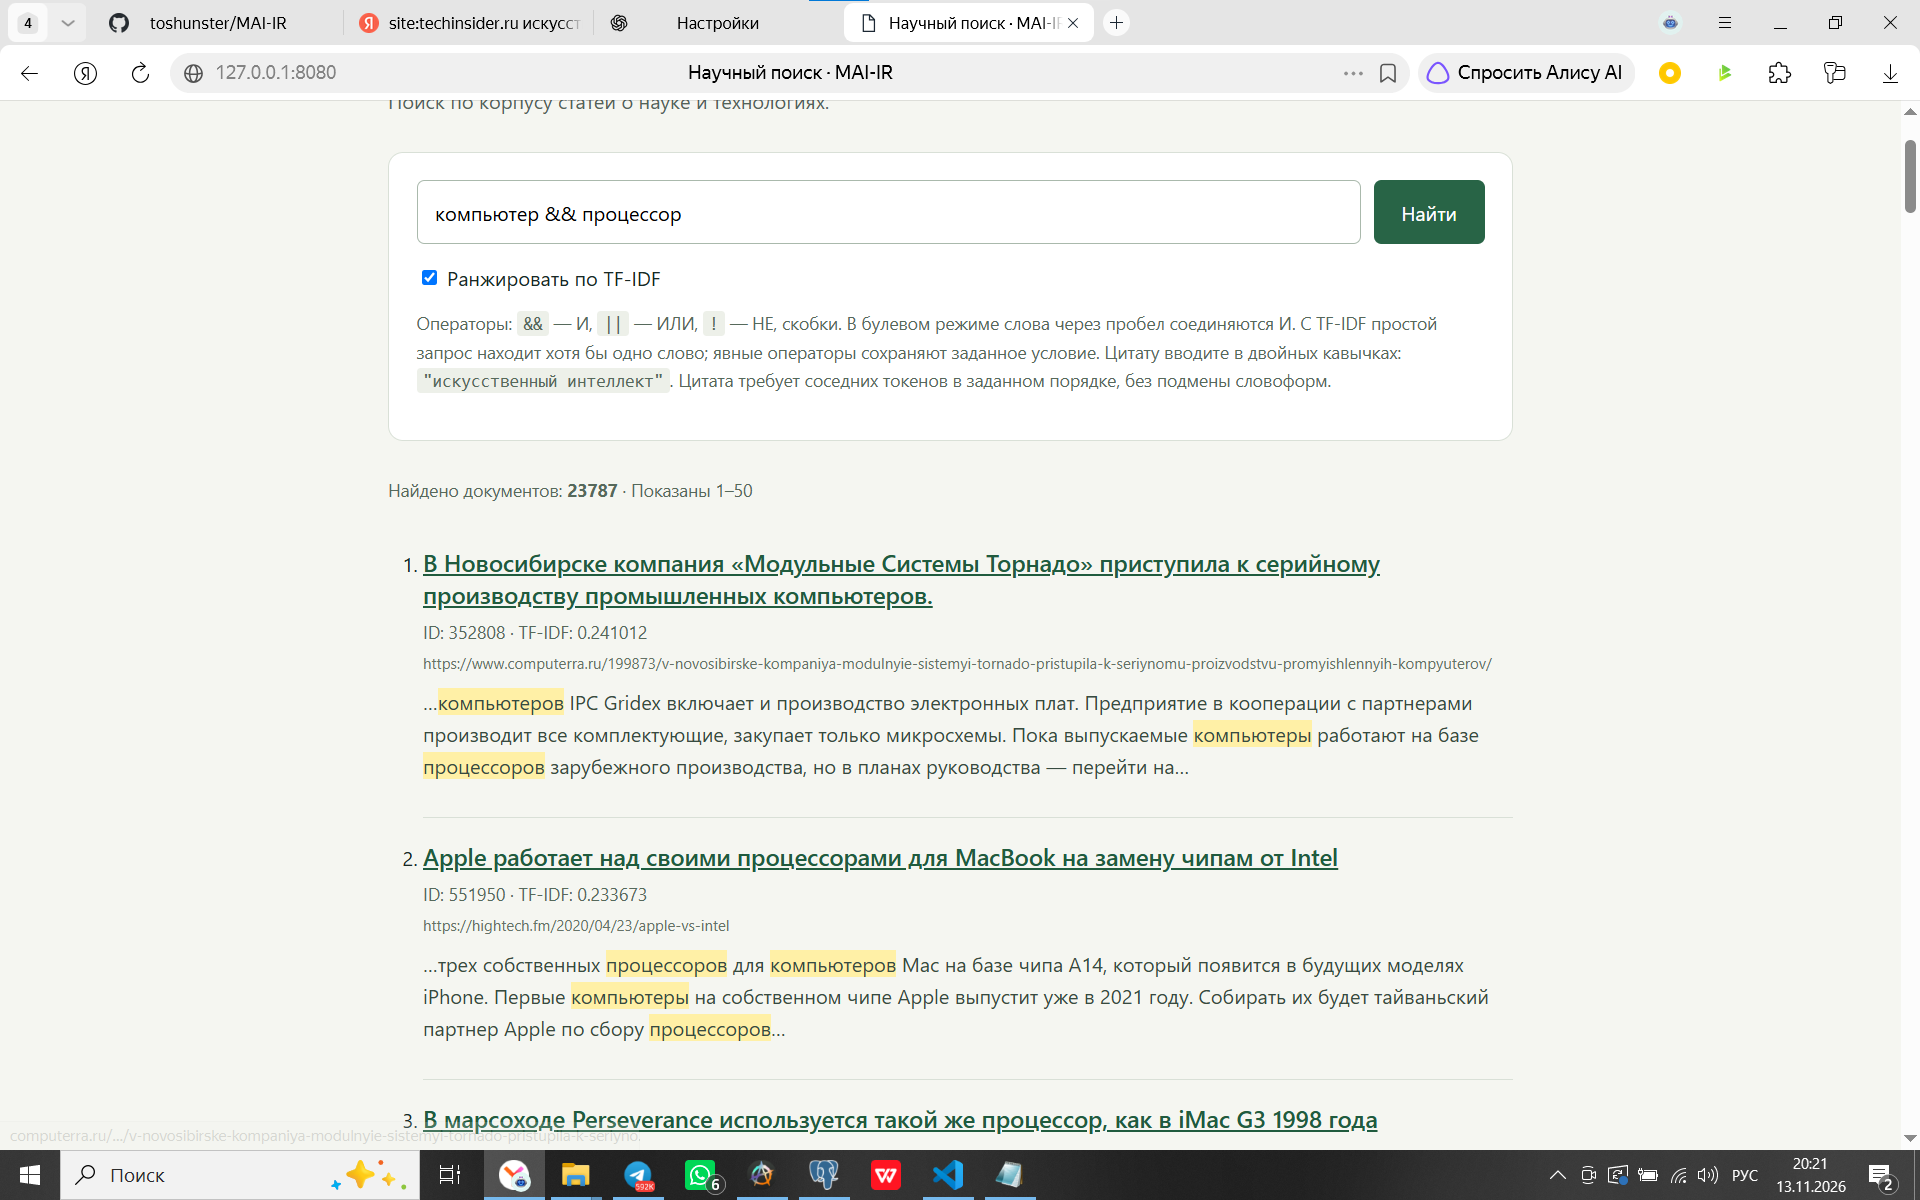
\includegraphics[trim={\ScreenshotLeft{} \ScreenshotBottom{} \ScreenshotRight{} \ScreenshotTop{}},clip,width=0.96\linewidth,height=0.70\textheight,keepaspectratio]{images/screenshots/lab14_snippets.png}
\endgroup\caption{Сниппеты исходного текста с подсветкой совпадений}\end{figure}

\section{Лабораторная работа № 17\\«Автотесты»}
\sub{Основания тестового плана}
Проверки покрывают отдельные функции C++, запуск консольных программ и HTTP-интерфейс. Ожидания получены из правил токенизации, эталонного словаря Snowball, операций над множествами и ручного расчёта весов TF-IDF. Проверяются обычные, граничные и ошибочные входы. Маленькие тестовые корпуса создаются автоматически; настоящий сетевой сбор не запускается.
\sub{Воспроизводимый прогон}
Команда \code{project.ps1 rebuild} собирает программы, запускает проверки, пересчитывает существующий экспорт корпуса, строит индексы, измеряет показатели и формирует этот отчёт. База для этого не требуется. \code{project.ps1 tests} выполняет только сборку и проверки; ошибки дают ненулевой код и сохраняются по группам. Логи находятся в \code{tests/results/}, подробные случаи --- в \code{tests_lr3_4/results/} и \code{tests_lr7_13/results/}.

\begin{table}[H]\centering\small
\caption{Покрытие компонентов автоматическими проверками}
\begin{tabularx}{\linewidth}{|p{0.18\linewidth}|X|p{0.17\linewidth}|}\hline
Компонента & Что проверялось & Уровень \\\hline
Токенизация & Регистр, ё, разделители, дефисы, аббревиатуры, ведущие нули, повторы и пустой ввод & UNIT, CLI \\\hline
Стемминг & Области и порядок правил, словоформы, смешанные токены, граница буфера, 49 785 эталонных пар & UNIT, CLI \\\hline
Индекс & Малый корпус, метаданные, пустые документы, дубли ID и повреждённые файлы & CLI \\\hline
Булев поиск & AND/OR/NOT, приоритеты, скобки, неизвестные термины, дополнение относительно всего корпуса & CLI \\\hline
TF-IDF & Независимый расчёт весов и норм, DF, повторы, отрицание, порядок результатов & CLI \\\hline
Сжатие & Обратимость и границы VB, ошибки кодека, совпадение постингов и полных выдач raw/VB & UNIT, CLI, полный корпус \\\hline
Веб & Форма, режимы, пагинация, экранирование HTML, ссылки и ошибки запроса & HTTP \\\hline
Частоты & Контрольные CF, порядок при равенстве, чтение строк и рост словаря & CLI \\\hline
Потоки & Эквивалентность файловому пути, метаданные, выравнивание токенов и основ & CLI \\\hline
Робот и конфиг & Лимиты, извлечение, сетевые ошибки, очередь, восстановление и настройки источников & Python unittest \\\hline
Лемматизация & Словарные формы, неизвестные токены, сохранение идентификаторов и числа вхождений & CLI \\\hline
Цитаты & Полная последовательность, порядок, повторы, пропуски, неизвестное слово, NOT/OR и независимый последовательный эталон & CLI \\\hline
Прыжки & Перезапуск VB на шагах 16/32/64, совпадение ответа с обычным пересечением, повреждение контрольной суммы & CLI \\\hline
Сниппеты & Исходные словоформы, подсветка совпадений и экранирование HTML & CLI, HTML \\\hline
\end{tabularx}\end{table}

\begin{table}[H]\centering\small
\caption{Фактический результат общего запуска}
\begin{tabularx}{\linewidth}{|X|r|r|r|}\hline
Группа & Сценариев & Код & Время, с \\\hline
linguistics\_unit & 27 & 0 & 0,061 \\\hline
linguistics\_cli & 38 & 0 & 0,716 \\\hline
linguistics\_contracts & 12 & 0 & 0,352 \\\hline
zipf\_cli & 16 & 0 & 0,505 \\\hline
search\_unit & 12 & 0 & 0,016 \\\hline
search\_cli & 37 & 0 & 3,697 \\\hline
web & 6 & 0 & 0,768 \\\hline
stream & 6 & 0 & 0,468 \\\hline
extensions & 18 & 0 & 0,922 \\\hline
collection & 88 & 0 & 2,455 \\\hline
\end{tabularx}\end{table}


\sub{Ограничения и итог проверки}
Все группы завершились кодом 0. Это подтверждает прохождение приведённого плана проверок. Подробные сценарии: \code{tests_lr3_4/TEST_PLAN.md} и \code{tests_lr7_13/TEST_PLAN.md}. Структура проекта и команды запуска приведены в \code{README.md}.
\begin{figure}[H]\centering\begingroup
\sbox{\ScreenshotBox}{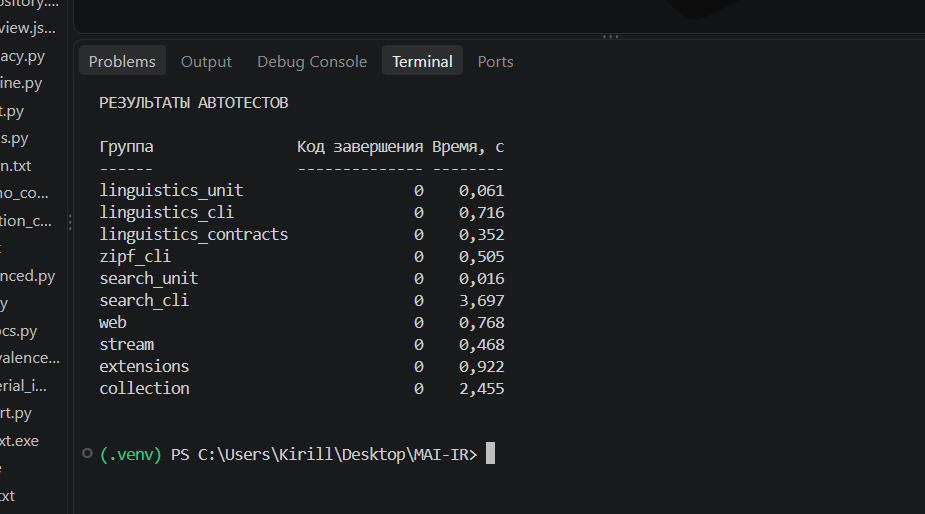
\includegraphics{images/screenshots/lab17_tests.png}}
\setlength{\ScreenshotLeft}{0.09945946\wd\ScreenshotBox}
\setlength{\ScreenshotBottom}{0.22178988\ht\ScreenshotBox}
\setlength{\ScreenshotRight}{0.41621622\wd\ScreenshotBox}
\setlength{\ScreenshotTop}{0.17704280\ht\ScreenshotBox}
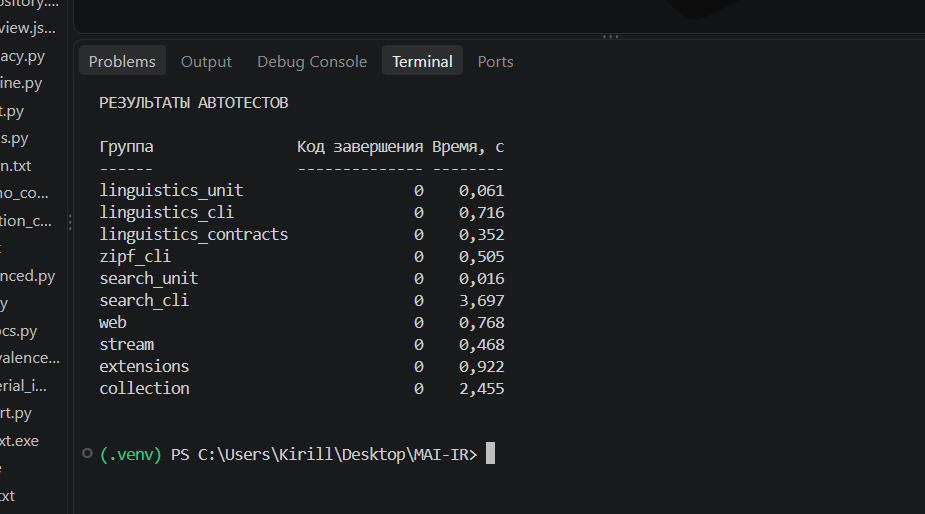
\includegraphics[trim={\ScreenshotLeft{} \ScreenshotBottom{} \ScreenshotRight{} \ScreenshotTop{}},clip,width=0.96\linewidth,height=0.70\textheight,keepaspectratio]{images/screenshots/lab17_tests.png}
\endgroup\caption{Результаты автоматических проверок}\end{figure}

\section{Итоговые результаты и развитие системы}
Реализован полный путь от сбора статей до веб-поиска: токенизация, стемминг и лемматизация, частотный анализ, бинарный индекс, булевы операции, строгие цитаты, сжатие, прыжки, TF-IDF и сниппеты. Этапы согласованы по ID, числу вхождений и контрольным суммам. Полные выдачи до и после сжатия совпали.

Дальнейшее улучшение --- независимая разметка большего числа запросов, разрешение неоднозначных слов по контексту и более информативный выбор фрагментов. Численные результаты сохранены в JSON/CSV, исходник отчёта --- \code{report.tex}.
\clearpage
\section{Источники и материалы}
\begin{enumerate}
\item Учебные материалы курса «Информационный поиск»: задания и лекции об индексации, сжатии и текстовом ранжировании. Планы проверок приведены в \code{tests_lr3_4/TEST_PLAN.md} и \code{tests_lr7_13/TEST_PLAN.md}.
\item Snowball: описание русского алгоритма и официальный тестовый словарь: \url{https://snowballstem.org/algorithms/russian/stemmer.html}; \url{https://github.com/snowballstem/snowball-data/tree/master/russian}.
\item OpenCorpora: словарные данные русского языка, \url{https://opencorpora.org/}. Происхождение данных записывается при подготовке словаря.
\item Manning, Raghavan, Schütze. Introduction to Information Retrieval: переменные байтовые коды и TF-IDF, главы 5--6: \url{https://nlp.stanford.edu/IR-book/}.
\item Собственный корпус: источники перечислены в таблице текущего снимка; фактические выводы C++-программ, JSON/CSV результатов и журналы автотестов в приложении к проекту.
\end{enumerate}
\sub{Репозиторий проекта}
Исходный код, результаты проверок и отчёт доступны в репозитории:
\begin{center}
\url{https://github.com/Fasko1/MAI-IR}\par\vspace{3mm}
\qrcode[height=23mm]{https://github.com/Fasko1/MAI-IR}
\end{center}
\end{document}
